\documentclass[german,english,twoside,headsepline,titlepage=true]{scrartcl}
% Header, der in jedem meiner Dokumente drinhängt.
% Setzt Rechtschreibung, Hyperlinks, Schriftart und Typographie

\usepackage[]{babel}
\babeltags{de = german}

\usepackage{xparse}
\usepackage[colorlinks=true,linkcolor=blue,pdfborder={0 0 0}]{hyperref}
\usepackage{hyperxmp}
\usepackage{microtype}
%\usepackage[scale=3]{ccicons}


\usepackage[]{fontspec}
%\setmainfont[Fractions=On]{Linux Libertine O}
\setmainfont{Linux Libertine O}
\setsansfont{Linux Biolinum O}

\usepackage{todonotes}
\usepackage[left]{showlabels}
% Hier sollten meine wichtigsten Mathe Befehle zu finden sein.
% Weiter unten sind die spezielleren Befehle, die je nach dem
% vielleicht auskommentiert oder gelöscht werden sollten.

\usepackage{amssymb}
\usepackage[]{amsmath}
\usepackage{amsthm}
\usepackage{mathtools}

%tikz
\usepackage{tikz}
\usetikzlibrary{shadows}
\tikzset{node distance=3cm, auto}
\usepackage{pgfplots}

%Abkürzungen für Standardzahlmengen
\let\C\relax
\NewDocumentCommand\R{}{\mathbb{R}}
\NewDocumentCommand\Q{}{\mathbb{Q}}
\NewDocumentCommand\N{}{\mathbb{N}}
\NewDocumentCommand\C{}{\mathbb{C}}
\NewDocumentCommand\Z{}{\mathbb{Z}}
\NewDocumentCommand\A{}{\mathcal{A}}
\NewDocumentCommand\K{}{\mathbb{K}}
\NewDocumentCommand\p{}{\mathbb{P}}
\NewDocumentCommand\h{}{\mathbb{H}}
\NewDocumentCommand\F{}{\mathcal{F}}
\NewDocumentCommand\D{}{\mathcal{D}}
\NewDocumentCommand\lie{}{\mathcal{L}}
\NewDocumentCommand\jo{}{\mathfrak{J}}
\NewDocumentCommand\hol{}{\mathcal{O}}
\NewDocumentCommand\mer{}{\mathcal{M}}
\NewDocumentCommand\diff{}{\mathcal{E}}

% ein Paar Abbildungssachen.
\NewDocumentCommand\Supp{}{\operatorname{Supp}}
\NewDocumentCommand\id{}{\operatorname{id}}
\NewDocumentCommand\supp{}{\operatorname{supp}}
\NewDocumentCommand\rank{}{\operatorname{rank}}
\NewDocumentCommand\tr{}{\operatorname{tr}}
\NewDocumentCommand\ord{}{\operatorname{ord}}

%Pfeile und Stuff
\NewDocumentCommand\Ra{}{\Rightarrow}
\NewDocumentCommand\La{}{\Leftarrow}
\NewDocumentCommand\LRa{}{\Leftrightarrow}
\NewDocumentCommand\ra{}{\rightarrow}
\NewDocumentCommand\la{}{\leftarrow}

% Faktorräume
\NewDocumentCommand\quot{m m}{\left .\raisebox{.2em}{$#1$}\middle/\raisebox{-.2em}{$#2$}\right .}

% richtiges epsilon und phi
\let\epsilon\relax
\NewDocumentCommand\epsilon{}{\varepsilon}
\let\phi\relax
\NewDocumentCommand\phi{}{\varphi}

% Differential
\let\d\relax
\NewDocumentCommand\d{ O{} }{\operatorname{d}\hspace{-0.1em}#1}

%amsthm
%\theoremstyle{plain}
\theoremstyle{definition}
\newtheorem{thm}{Satz}[section]
\newtheorem{lemma}[thm]{Lemma}
\newtheorem{prop}[thm]{Proposition}
\newtheorem{cor}[thm]{Korollar}
%\theoremstyle{definition}
\newtheorem{defin}[thm]{Definition}
\newtheorem{bsp}[thm]{Beispiele}
%\theoremstyle{remark}
\newtheorem{rem}[thm]{Bemerkung}

% % Differentialgeometrie (Riemannsche Geometrie)
% \NewDocumentCommand\tang{ O{p} O{M}}{T_{#1}#2}
% \NewDocumentCommand\cotang{ O{p} O{M}}{T^\ast_{#1}#2}
% \NewDocumentCommand\del{ O{i} O{x} O{} }{\frac{\partial {#3}}{\partial {#2}^{#1}}}
% \NewDocumentCommand\delat{ O{p} O{i} O{x} O{} }{\left . \del[#2][#3][#4] \right |_{#1}}
% \NewDocumentCommand\christ{O{i} O{j} O{k} }{ \Gamma_{#1 #2}^{#3} }
% \NewDocumentCommand\g{m m}{\langle #1, #2 \rangle}
% \NewDocumentCommand\diam{}{\operatorname{diam}}
% \NewDocumentCommand\ric{}{\operatorname{ric}}
% \NewDocumentCommand\scal{}{\operatorname{scal}}
% \NewDocumentCommand\arsinh{}{\operatorname{arsinh}}

% % Bachelor-Arbeit
% \NewDocumentCommand\im{}{\operatorname{im}}
% \NewDocumentCommand\sm{}{\operatorname{sm}}
% \NewDocumentCommand\Reg{}{\operatorname{Reg}}
% \NewDocumentCommand\be{}{\mathfrak{B}}
% \NewDocumentCommand\pe{}{\mathfrak{P}}
% \NewDocumentCommand\res{}{\operatorname{res}}
% \let\S\relax
% \NewDocumentCommand\S{}{\mathcal{S}}
% \let\P\relax
% \NewDocumentCommand\P{}{\mathbb{P}}
% \NewDocumentCommand\Fix{}{\operatorname{Fix}}
% \NewDocumentCommand\Mat{}{\operatorname{Mat}}
% \NewDocumentCommand\SL{}{\operatorname{SL}}
% \NewDocumentCommand\GL{}{\operatorname{GL}}
% \NewDocumentCommand\PSL{}{\operatorname{PSL}}
% \let\Re\relax
% \NewDocumentCommand\Re{}{\operatorname{Re}}
% \let\Im\relax
% \NewDocumentCommand\Im{}{\operatorname{Im}}
% \NewDocumentCommand\Div{}{\operatorname{Div}}
% \NewDocumentCommand\Aut{}{\operatorname{Aut}}
% \NewDocumentCommand\Deck{}{\operatorname{Deck}}
% \NewDocumentCommand\runge{}{\mathfrak{h}}
% \NewDocumentCommand\fu{}{\mathfrak{U}}
% \NewDocumentCommand\dist{}{\mathcal{D}}

% Header, für sowas wie Bachelor- oder Master-Arbeiten.
% Folgende Parameter sind für documentclass vielleicht hilfreich:
% twoside: zweiseitiger Satz
% headsepline: Kopfzeile wird durch langen Strich getrennt
% titlepage = true: Es gibt eine Titel Seite und nicht nur ein Überschrift
% BCOR = 10mm: Binderandkorrektur einstellen

\usepackage{scrpage2}
\pagestyle{scrheadings}
% \ofoot{\pagemark}
% \lehead{Ich stehe in header\_artcl unter lehead}
% \rohead{\headmark}
\automark[subsection]{section}
%\automark*[subsection]{}

\usepackage[style=alphabetic,backend=biber]{biblatex}
\addbibresource{biblio.bib}

% \usepackage{makeidx}

% \NewDocumentCommand\init{m}{\emph{#1}\index{#1}}

% \makeindex

%%% Local Variables:
%%% mode: plain-tex
%%% TeX-master: "Bachelor"
%%% End:



\usepackage{chemformula}
\usepackage[exponent-product = \cdot]{siunitx}
\usepackage{graphicx}
\usepackage{booktabs}
\usepackage{float}
\graphicspath{ {images/} }


% \usepackage{gnuplottex}
\newfontfamily\nfrac[Fractions=On]{Linux Libertine O}
%\newfontfamily\diagram[Size=.5]{Linux Libertine O}

\usepackage{pgfplots}

\usepackage{ccicons}

\addfontfeature{Fractions=On}

% Schmutztitel
\KOMAoption{twoside}{false}
\extratitle{
  ~
  \begin{center}
    \huge \textbf{Department of Physics \& Astronomy}
  \end{center}
  ~
  \begin{center}
    \Large \textbf{Heidelberg University}
  \end{center}
  \vfill
  \begin{center}
    \Large \textbf{Bachelor Thesis}\\[1ex]
    in the degree program Physics (B.\,Sc.)\\
    submitted by\\[1ex]
    \Large \textbf{Tim Adler}\\[1ex]
    born in Sinsheim (Germany)
  \end{center}
  ~
  \begin{center}
    \huge \textbf{2016}
  \end{center}
}

\KOMAoption{twoside}{true}

\titlehead{Heidelberg University \\
  Department of Physics \& Astronomy\\
  Im Neuenheimer Feld 226\\
  69120 Heidelberg\\
  Germany}
\subject{Bachelor Thesis}
\title{Ein Konverter}
\author{Tim Adler}
\date{April 25, 2016}
\publishers{Advised by\\Dr.\ Denis Pöhler, Dr.\ Martin Horbanski\\and Prof.\ Dr.\ Ulrich Platt}
\uppertitleback{Tim Adler\\Eberlinweg 6\\69121
  Heidelberg\\Germany\\tim \{at\} emrys-merlin.de}
\lowertitleback{
\textbf{Ein Konverter}\\
Bachelor Thesis in the degree program Physics (B.\,Sc.)\\[\baselineskip]
Heidelberg University\\
Department for Physics \& Astronomy\\
Institute for Environmental Physics\\[\baselineskip]
\begin{tabular}[htbp]{l l}
Advised by & Dr.\ Denis Pöhler, Dr.\ Martin Horbanski and Prof.\ Dr.\ Ulrich Platt\\
Starting date & January 17, 2016 \\
Closing date & April 25, 2016\\
\end{tabular}
\\[\baselineskip]
\ccbysa\vspace{0.2cm}\\
This thesis is licensed under a
Creative Commons Attribution-ShareAlike 3.0 Unported License. See
\url{http://creativecommons.org/licenses/by-sa/3.0/} for more information.\\[\baselineskip]
This work has been set using {\LaTeX} and {\KOMAScript}.\\[\baselineskip]
\begin{tabular}[htbp]{r l}
  Main Font: & Linux Libertine O\\
  Sans Font: & Linux Biolinum O
\end{tabular}}

\makeatletter
\hypersetup{
  pdftitle={\@title},
  pdfauthor={\@author},
  pdfdate={\@date}
}
\makeatother

\begin{document}

\pagenumbering{roman}
\selectlanguage{german}
\maketitle
\selectlanguage{english}

\listoftodos
\todo{ToDo-Liste entfernen.}
\todo{check indention after formulas.}
\newpage

\selectlanguage{german}

\subsubsection*{Zusammenfassung}
\label{sec:Zusammenfassung}

Ich mach was zu Konvertern
\todo{Zusammenfassung schreiben}

\selectlanguage{english}

\subsubsection*{Abstract}
\label{sec:abstract}

I try to build some sort of converter
\todo{Write abstract}

%%% Local Variables: 
%%% mode: latex
%%% TeX-master: "../Bachelor"
%%% End: 

\newpage

% Nur bis section, nicht bis subsection
\setcounter{tocdepth}{2}
\tableofcontents
\cleardoubleoddstandardpage{}
\pagenumbering{arabic}
Nothing to see yet
\cleardoubleoddstandardpage{}
\section{Theoretical background}
\label{sec:theory}

\subsection{Ozone chemistry and \ch{NO} to \ch{NO2} conversion}
\label{sec:chemistry}

This section lays the chemical groundwork for the construction of our
\ch{NO} to \ch{NO2} converter. First we will introduce the rate
coefficient to get a measure for the speed of a
reaction. Afterwards we will have a look at possible ways to generate
Ozone out of ambient air and then describe Ozone induced reactions
concerning Nitrogenoxides. This section is mainly inspired by and
taken from~\cite{bsc}.

\subsubsection{The rate coefficient}
\label{sec:rate}

During our conversion we will have many chemical reactions of the form

\begin{align*}
  \ch{A + B -> C + D}.
\end{align*}

Some of them will have positive, wanted effects, others describe side
effects and we want to suppress them as much as possible. However we
have only two parameters we can vary. The first is the Ozone
concentration, which we can vary slighty and very roughly and the
other one is the reaction pathlength and by that the reaction
time. Thus our best chance to select certain reactions is to set ther
reaction time to a value that corresponds to the different reaction
speeds of the equations, making sure that wanted reactions have enough
time to happen while simultaneously having the time too short for
unwanted reactions. Of cours this is only possible, if the wanted
reactions run faster than the unwanted ones. 

With this motivation in mind, we need a measure for the reaction
speed. Thinking of speed in this setting means to think of change of
compound concentration. In this section we will use $c$ to denote
concentrations. Using the above mentioned prototypic equation, we can
see that the change of concentration, i.\,e. $\dot c$, of the
different species are related by:
\begin{align*}
  -\dot c(A) = - \dot c(B) = \dot c(C) = \dot c(D).
\end{align*}

Lastly we want to get a connection of these derivatives to the educt
concentration. The probability for a reaction to take place should be
proportional both to $c(A)$ and $c(B)$ as the two particles need to
`meet'. Thus we expect
\begin{align}
  -\dot c(A) = - \dot c(B) = k \cdot c(A) \cdot c(B), \label{eq:rate}
\end{align}

where the proportionality constant $k$ ist called \emph{rate
  coefficient}. It is often given in units of
\si{\hertz\per\cubic\centi\meter}. This $k$ is our desired reaction
speed measure, as it describes concentration independently the
reaction time. 

In our case the Ozone concentration will often far exceed the
concentration of the other trace gases. This allows us to think of its
concentration as approximately constant. If we set $c(B)$ constant in
Equation~\eqref{eq:rate}, then we get a well known ordinary first
order differential equation with solution
\begin{align*}
  c(A,t) = c(A,0)\exp(kc(B)\cdot t).
\end{align*}

In this limiting case we see that the decay time is given by $\tau =
(kc(B))^{-1}$, such that the connection of $k$ to the reaction speed
becomes obvious.

\subsubsection{Ozone Generation}
\label{sec:theory-ozone}

In this section we will discuss the generation of Ozone (\ch{O3}) out of ambient
air. The main idea comes from the observation that stratospheric
\ch{O3} protects us from ultraviolet (UV) light. Thus Ozone needs to
have absorption bands there. Furthermore normally the Ozone layer is
not depleted, but regenerates itself, so there needs to be a reaction
cycle building Ozone out of ordinary Oxigen molecules (\ch{O2}).

The following equations describe the processes using UV photons to
generate and destroy Ozone. The cycle is ofthen referred to as
\emph{Chapman-Cycle}\todo{cite}. In some of the reactions an
additional molecule is necessary to assure momentum conservation. This
inert reaction participant is always denoted \ch{M}.

The first part of the cycle contains the reactions, that generate
\ch{O3} out of \ch{O2}

\begin{align}
  \ch{O2} + h\nu &\ch{-> 2 O(^3P)},\nonumber\\
  \ch{O(^3 P) + O2 + M} &\ch{-> O3 + M}. \label{eq:ozone}
\end{align}

We see that a photon splits an Oxygen molecule and the excited
Oxygen atom reacts with another \ch{O2} molecule to form Ozone. For
the first reaction to take place we need for the wavelength of the
photon $\lambda < \SI{242}{\nano\meter}$ to hold, i.\,e.\ we need a UV
photon. 

The next part of the cycle shows, how another UV photon can destroy
Ozone and create a ground state Oxygen atom. This Oxygen atom will
then be reexcited:

\begin{align}
  \ch{O3} + h\nu \ch{&-> O(^1 D) +
  O2}, \label{eq:split}\\
  \ch{O(^1 D) + M & -> O(^3 P) + M}.\nonumber
\end{align}

After this reaction there are two possible parts. Firt the $\ch{O}(^3
P)$ can reenter into Equation~\eqref{eq:ozone}, such that there is no
net change in Ozone or it could react to form \ch{O2} by the
following mechanisms

\begin{align*}
  \ch{2 O(^3 P) + M & -> O2 + M} \quad \text{and}\\
  \ch{O(^3 P) + O3 & -> 2 O2},
\end{align*}

leading to a net loss of Ozone. Introducing a UV light source with
wavelength less than \SI{242}{\nano\meter} will start the above
cycle. Since it contains sources and sinks for Ozone, we will reach an
equilibrium state with a limiting Ozone concentration. This
concentration will depend on multiple factors, which influence the
reaction speeds. First and foremost the intensity of the light source
at different wavelength segments determines if more Ozone is generated
than destroyed or not. An in depth analysis of this reaction system
has been carried out by\todo{cite}. For this work the main conclusion
is sufficient that using a Pen-Ray Hg-lamp within an alluminium coated
tube shifts the equilibrium in the above equations to a point where
there is enought Ozone generated for our purposes. The exact
characteristics of our generator were determined experimentally and
the results can be found in Section~\ref{sec:ozone}. 

\subsubsection{Ozone triggerd Nitrogenoxide reactions}
\label{sec:o-no}

In this section we will have a look at all reactions concerning
chemicals consisting of Nitrogen and Oxygen. Our aim is to convert
100\% of the Nitrogenmonoxide (\ch{NO}) to Nitrogendioxide
(\ch{NO2}). However introducing Ozone to the sample air can trigger
other reactions. If these lead to a net change of \ch{NO2} we have
additional effects to correct, if we want to determine the \ch{NO}
concentration. All reactions are given with their corresponding rate
coefficient $k$ which were taken from~\cite{bsc}. In
Section~\ref{sec:requirements} we will discuss the implications of the
reactions here on the setup of our converter.

The reaction we are mainly interested in and we want to be dominant is
the following

\begin{align*}
  \ch{NO + O3 & ->[$k=\SI{1.8e-14}{\hertz\per\cubic\centi\meter}$] NO2 + O2}.
\end{align*}

If this were the only reaction, we would have a one to one conversion
from \ch{NO} to \ch{NO2}. We would only have to make certain that
there is enough Ozone. However this is not the only reaction taking
place. Nitrogendioxide itself can be oxidized by Ozone to generate
Nitrogentrioxide (\ch{NO3}):

\begin{align*}
  \ch{NO2 + O3 ->[$k=\SI{3.5e-17}{\hertz\per\cubic\centi\meter}$] NO3 + O2}.
\end{align*}

Luckily, we see that the rate coefficients of the two reactions are
very different and the first ony is approximately three orders of
magnitude faster than the second one. Furthermore \ch{NO3} is again
not detectible by our measurement instrument. Also \ch{NO3} can react
again with \ch{NO2} to generate laughing gas

\begin{align}
  \ch{NO2 + NO3 + M
  <=>[$k=\SI{1.9e-12}{\hertz\per\cubic\centi\meter}$][$k=\SI{2.6e-11}{\hertz\per\cubic\centi\meter}$]
  N2O5 + M}. \label{eq:laughing}
\end{align}

As we can see the equilibrium of Equation~\eqref{eq:laughing} lies on the
side of the educts, so the effect should not be too large, if the
\ch{NO3} concentration can be kept low. In addition there is another
very fast reaction using \ch{NO3}

\begin{align}
  \ch{NO + NO3 ->[$k=\SI{6.9e-2}{\hertz\per\cubic\centi\meter}$] 2 NO2}.\label{eq:back}
\end{align}

Thus, if we keep the Nitrogentrioxide concentration low to begin with,
the above reaction implies that basically all of it should react with
\ch{NO} to form \ch{NO2}. Since \ch{NO3} is quickly destroyed by
photolysis, we can assume our measurement air to be \ch{NO3} free (at
least during day time measurements). Thus the molecules come either
from oxidizes \ch{NO2} or from twice oxidized \ch{NO}. In both cases
Equation~\eqref{eq:back} makes sure that our measurement is not distorted.


\subsection{Basics of fluid dynamics}
\label{sec:fluid}

One important aspect of this work consists in the understanding of the
different gas flows in the instrument. We need an estimate for the
mixing time of Ozone with the sample air and then we need to know how
long our mixing and reaction pathlength needs to be in order to
achieve a full conversion. These questions can all be answered using a
few basic principles from fluid dynamics. First we will have a look at
laminar flows in cylindric vessels (in our case tubes) to get a
connection between the flow and the maximum speed in the tube. Next we
have a look at diffusion of gases. As we only hav laminar flows,
diffusion is the only way mixing can take place, so we need an
estimate of the time this mixing takes. Lastly we will discuss
adsorption of some trace gases at teflon, silica gel and activated
carbon to better our understanding of the filtering effects in the
instrument. 

\subsubsection{Laminar flows in cylinders}
\label{sec:cylinder}

We are interested in what regime the gas transport in the tube
remains. Especially after the ozone enriched air is added to the
sample air, we would benefit from ab turbulent flow in the system as
it would acertain a faster mixing of the gases. To see whether we have
a laminar or a turbulent flow, we use the phenomenological \emph{Reynold's
number}

\begin{align*}
  \operatorname{Re} = \frac{\rho \cdot d \cdot \bar v}{\eta},
\end{align*}

where $\rho$ denotes the density of our gas, $d$ is a characteristc
length of the system, in our case the tube diameter, $\bar v$ is the
average velocity of the gas and $\eta$ its viscosity. As a rule of
thumb the flow in a cylinder will be laminar, if the Renold's number
is smaller than the critical Reynold's number
$\operatorname{Re}_{\text{c}} = 2300$ and the flow will be turbulent
if the number is higher than $3000$ (c.\,f.~\cite{maschbau}). In our
system we have $d = \SI{4}{\milli\meter}$, $\rho \approx
\SI{1.2}{\kilo\gram\per\cubic\meter}$ and $\eta \approx
\SI{17.1}{\micro\pascal\second}$. Furthermore we work with a flow of
$\Phi = \SI{2}{\liter\per\minute}$. With the above diameter this
leads to an average velocity of $\bar v =
\SI{2.7}{\meter\per\second}$. Using this data we compute the Reynold's
number to be

\begin{align*}
  \operatorname{Re} \approx 760 < 2300.
\end{align*}

Thus we see that we work solely in the laminar setting and we need to
understand the velocity distribution in this case in order to allow
enough time for mixing and the chemical reactions to take place. The
law behind the flow in a cylindric tube is called
\emph{Hagen-Poiseulle} and we follow the exposition used
in~\cite{gerthsen} to derive it.

Denote by $r_0$ the inner radius of our tube and by $l$ its length. We
assume that we are in the equilibrium state, such that all forces need
to add to zero. We look at a cylinder with radius $0 \leq r \leq
r_0$. To have a nonzero flow, we need a pressure difference at the two
ends of the tube dentode $\Delta p$. The force exerted on the cylinder
by the pressure is given by
\begin{align*}
  F_b = - \pi r^2 \Delta p,
\end{align*}

where the minus sign is introduced because the force points in the
opposite direction of the pressurre gradient. On the boundary of our
cylinder we have friction. The force exerted by 
it is proportional to the area of friction, i.\,e.\ the cylinder
barrel and to difference in velocity between the fluid within the
cylinder and without, since we have to look at an infinitesimal anulus
around the boundary, we get a proportionality to the velocity gradient
$\frac{\d[v]}{\d[r]}$. Thus the force of friction takes the form

\begin{align*}
  F_f = \eta \cdot 2\pi r \cdot l \cdot \frac{\d[v]}{\d[r]}.
\end{align*}

We are at an equilibrium state, thus we need $F_b = F_f$ for all
possible $r$ to hold. This leads us to the following differential
equatio for the velocity

\begin{align*}
  \frac{\d[v]}{\d[r]} = - \frac{\Delta p}{2l\eta} r
\end{align*}
 
whic can be directly integrated. Using the boundary condition $v(r_0)
= 0$, i.\,e.\ the fluid sticks at the wall of the tube, we yield

\begin{align}
  v(r) = v_0 \left ( 1 - \left( \frac{r}{r_0} \right)^2 \right) \quad
  \text{with }\ v_0 \coloneqq \frac{\Delta p r_0^2}{4 l \eta}. \label{eq:v}
\end{align}

This can be further integrated to yield the flow $\Phi$ of the system

\begin{align*}
  \Phi = \int_A v(r) \d[A] = 2\pi \int_0^{r_0} v(r)r \d[r] = \frac{\pi
  r_0^4}{8\eta l} \cdot \Delta p.
\end{align*}

This is the standard form of the Hagen-Poiseulle law. One remarkabel
obersvation is that there is a power four law between the radius of
the tube and the flow. More interesting for us is the relation between
the average velocity $\bar v$ and the maximum velocity $v_0$ at the
center of the pipe

\begin{align*}
  \bar v = \frac{\Phi}{\pi r_0^2} = \frac{\Delta p r_0^2}{8\eta l} \stackrel{\eqref{eq:v}}{=} \frac{v_0}{2}.
\end{align*}

So we see that at the center the the velocity is twice as large as the
average. We need to keep this effect in mind when it comes to compute
the dwell time of our gases.

\subsubsection{Diffusion}
\label{sec:diffusion}

As was shown in the previous section, the gas flows laminarly through
our instrument. Thus the only mechanism by which gas mixing can occur
is \emph{diffusion}. Therefore we we want an estimate for the time it
takes for diffusion to take place. This exposition drew inspiration
from~\cite{fluid}.

We are interested in the evolution of the concentration $n$ of a
species. Fick's first law states that the flow $\Phi$ of the species
is proprotional to the concentration gradient $\nabla n$ and that the
species flows from higher to lower concentration. We yield

\begin{align*}
  \Phi = - D \nabla n,
\end{align*}
where $D > 0$ is called the \emph{diffusion constant}. Assuming no
sources and sinks and using the continuity equation for fluids, we
arrive at Fick's second law

\begin{align*}
  \dot n = - \nabla \Phi = \nabla (D \nabla n) = D \cdot \Delta n,
\end{align*}
where for the last equation we assumed and istotrope medium, i.\,e.\
$\nabla D = 0$. This is a second order linear partial differential
equation and for arbitrary boundary conditions it can become
arbitrarily hard to solve. Since we are mostly interested in the
diffusion of species at small time scales, we can assume our vessel
inifinitely large. With this the equation becomes accessible via
Fourieranalysis. Let

\begin{align*}
  \hat n(k,t) = \mathcal{F}[n](k,t)
\end{align*}
be the fouriertransform of $n$ with regard to the three spatial
coordinates $x$. Using the known relation $\mathcal{F}[\partial_{x_j}
n](k,t) = -ik_j \hat n(k,t)$, we can transform the equation to

\begin{align*}
  \partial_t \hat n(k,t) =  - Dk^2 \hat n(k,t)
\end{align*}

an linar first order ordinary differential equation, with the well
known solution

\begin{align}
  \hat n(k,t) = c(k) \cdot \exp(-Dk^2 t). \label{eq:sol-ft}
\end{align}

To determine $c(k)$, we need to introduce an initial value. We again
work with an idealistic model. We will later on be interested in the
diffusion of one molecule. Therefore we work with the initial
condition
\begin{align*}
  n(x,0) = n_0 \delta(x),
\end{align*}
i.\,e.\ all the species (or for $n_0 = 1$: the particle) is localized
at one point for $t = 0$. We can fourietransform this initial
condition, too, and yield

\begin{align*}
  \hat n(k,0) = n_0.
\end{align*}
Plugging this into Equation~\eqref{eq:sol-ft}, we get

\begin{align*}
  \hat n(k,t) = n_0 \exp(-Dt \cdot k^2).
\end{align*}
This is a Gaußian function with regard to the variable $k$. If we want
the solution in terms of $x$ we need the inverse Fourier transform of
$\hat n$. However, we know that the Gauß function is an Eigenfunction
of the Fouriertransform (and its invers). Additionally the total
concentration needs to be the same for all times $t$. Thus we yield

\begin{align*}
  n(x,t) = \frac{n_0}{(2\pi \cdot 2Dt)^{3/2}} \cdot \exp \left(
  -\frac{1}{2} \cdot \frac{x^2}{2Dt} \right).
\end{align*}
We have found the solution to Fick's second law. This allows us to
describe the statistic behaviour of a particle undergoing
diffusion. Setting $n_0 = 1$, we arrive at the probability
distribution for the particle, which is just a Gaußian distribution
with a timedependent variance. We see that the expectation value of
the position $\langle x \rangle$ is always 0. However the standard
deviation $\sigma = \sqrt{2Dt}$
grows larger over time, such that vor the \emph{mean squared
  displacement}, we yield the following relation

\begin{align}
  \langle x^2 \rangle = \sum_{j=1}^3 \langle
  x_j^2 \rangle = \sum_{j=1}^3 \sigma^2 = 3 \cdot 2Dt, \label{eq:mqd}
\end{align}

where we used $\langle x \rangle = 0$. This mean squared displacement
can now be used as a measure to gauge the distance travelled by a
molecule. We will apply it to gauge the time needed for a new gas
species (in our case Ozone) to fill a volume sufficiently for the
chemical reactions to take place.

\subsubsection{Adsorption}
\label{sec:adsorption}
\todo{find something out and write something about diffusion}

\subsection{Technical requirements for the converter}
\label{sec:requirements}

The above considerations lead to some technical requirements in the
construction of our converter. First and obviously we need to use well
filtered air in the Ozone generator as not to introduce other trace
gases which would disturb the measurement. The normal procedure
consists of using an activated charcoal, a silica gel and a particle
filter. However, one problem is that \ch{NO} is hardly soluble in
water and thus passes all these filter barriers. After the Ozone
generation it will react with it and lead to an additional \ch{NO2}
signal, which cannot be neglected. To remove it, one can add
another silica gel filter after the generator. \ch{NO2} is well
adsorbed within, which should lead to the desired reduction of the
error. However, Ozone is also adsorbed in Silica. Luckily, the
adsorption capacity for Ozone is much worse than for Nitrogen
Dioxide. So we would expect the filter to be quickly saturated by
Ozone, so that it can pass, while still blocking \ch{NO2}. To make
this work, we also have to add some extra pathlength after the
generator to make sure that the oxidization takes place before the gas
passes the Silica gel filter.

The next restriction is that we need a nigh \SI{100}{\%} conversion of
\ch{NO} to \ch{NO2}. This leads to three considerations. Firstly, we
need enough time for the mixing of the ozone with the sample air to
take place. Secondly, we need enough time for the actual reaction to
take place. Thirdly, we need the time to be short enough, such that we
do not loose to much \ch{NO2} to further oxidation.

Concering our first consideration, we have to look at
Section~\ref{sec:fluid} to estimate the mixing time. As we work with
laminar flows in the reaction path (c.\,f.\ Sec.~\ref{sec:cylinder}),
the mixing will be dominated by diffusion. Thus we use the mean
squared displacement to estimate the time the Ozone takes to cross the
tube diameter. In our case we use tubes with $d =
\SI{4}{\milli\meter}$ and the diffusion constant for Ozone in air was
taken to be $D = \SI{0.137}{\square\centi\meter\per\second}$ (at $T =
\SI{298}{\kelvin}$ and $p = \SI{1}{\text{bar}}$
c.\,f.~\cite{diff-ozone}). With these values we get
\begin{align*}
  t_{\text{mix}} = \frac{d^2}{6\cdot D} = \SI{0.195}{\second}
\end{align*}

Turning towards considerations two and three, we need to gauge the
reaction times. For this we have to set a desired conversion
ratio. For our estimates work with a ratio of \SI{99}{\%}. 
Since the Ozone generator will supply an
overabundance of \ch{O3}, we can use the linear ordinary
differential equation approximation introduced in
Section~\ref{sec:rate}. Thus the conversion ratio is
given by
\begin{align*}
  \exp(-kc(\ch{O3})\cdot t),
\end{align*}
where $t$ is the reaction time. $1$ stands for no
conversion at all (i.\,e.\ no decrease in the educt concentration) and
$0$ stands for complete conversion. For \SI{99}{\%} we need
\begin{align}
  kc(\ch{O3}) \cdot t_{\text{react}} \gtrsim 4.6. \label{eq:react-bound}
\end{align}
As a lower bound for the Ozone concentration we use
\begin{align*}
  c(\ch{O3}) = \SI{2}{ppm} = \SI{4.996e13}{\per\cubic\centi\meter} 
\end{align*}
and using $k = \SI{1.8e-14}{\hertz\per\cubic\centi\meter}$, we yield
the following natural time scale
\begin{align*}
  \tau^{-1} & = k c(\ch{O3}) = \SI{0.90}{\hertz}.
\end{align*}

Together with Equation~\eqref{eq:react-bound} this leads to

\begin{align*}
  t_{\text{react}} \gtrsim \SI{5.1}{\second}.
\end{align*}

Using $t_{\text{react}}$ to compute the conversion ratio of
$\ch{NO2}$ to $\ch{NO3}$, we get \SI{0.9}{\%}. So with this reaction
time we should expect about a \SI{2}{\%} error in the retrieved
\ch{NO} concentration. Hopefully, the results will be better than
that, as some of the produced \ch{NO3} will (as described in
Section~\ref{sec:o-no}) quickly degrade to \ch{NO2} and the Ozone
concentration is likely to be underestimated.

As a last step we want to translate the needed mixing and reaction
time
\begin{align*}
  t = t_{\text{mix}} + t_{\text{react}} = \SI{5.3}{\second}
\end{align*}
to be converted to its associated pathlength. Using the applied flow
of $\Phi = \SI{2}{\liter\per\minute}$, we can compute the average
speed of the gas to be
\begin{align*}
  \bar v = \frac{\Phi}{\pi r^2} = \SI{2.7}{\meter\per\second}. 
\end{align*}
As was described in Section~\ref{sec:cylinder} this corresponds to a
maximal speed in the center of the tube of

\begin{align*}
  v_0 = 2\cdot \bar v = \SI{5.4}{\meter\per\second}.
\end{align*}

Using these two speeds we get

\begin{align*}
  \bar l & = \SI{14.31}{\meter} \quad \text{and}\\
  l_0 & = \SI{28.62}{\meter}
\end{align*}
as our pathlengths.

For the experiment we oriented at $\bar l$, as the maximum speed is
only relevant for a rather small cross section of the
cylinder. Most experiments were performed at $l = \SI{10}{\meter}$
accepting a slightly worse \ch{NO} conversion ratio at the upside of a
smaller loss to \ch{NO3}. As all these estimates were intended as a
worst case, we expect even a \SI{10}{\meter} reaction path to be
sufficient for acceptable results.

\subsection{The physics behind CE-DOAS}
\label{sec:ce-doas-physics}

In the following sections we will discuss the physical concepts
necessary to understand the Cavity Enhance Diffirential Absorption
Spectroscopy (CE-DOAS). First, we will investigate the Lambert-Beer
Law. This leads directly to the so called \emph{Longpath}-DOAS
instrument. As the name already indicates, those need a long
lightpath, since normally the absorption crosssections are very
small. Thus lastly we introduce the \emph{cavity enhancement} to
overcome this restriction.

The presentation follows mostly~\cite{fp58} with a few inspirations
taken from~\cite{bsc} and~\cite{platt2008differential}.

\subsubsection{The Lambert-Beer Law}
\label{sec:lambert-beer}

The \emph{Labert-Beer Law} ist the underlying principle behind the
main measurement method used in this work. It concerns itself with the
evolution of the light intensity $I_0$ which propagates a certain
distance $L$ through air. It assumes an exponential decay over $L$, so
we can write

\begin{align}
  I(\lambda, L) = I_0(\lambda) \cdot \exp[-\epsilon(\lambda) \cdot
  L], \label{eq:lb-easy}
\end{align}

where $\epsilon$ is called \emph{absorption coefficient}. This
coefficient contains all the influences of the matter on the
absorption and can thus be split to account for the different
absorption and scattering mechanisms:

\begin{align*}
  \epsilon = \epsilon_a + \epsilon_R + \epsilon_M,
\end{align*}

where $\epsilon_a$ denotes the absorption and scattering due to the
trace gases, $\epsilon_R$ denotes Rayleigh scattering and $\epsilon_M$
Mie scattering. Next we want to understand the influence of the trace
gases on $\epsilon_a$ a little better. The absorption should be
proportional to the concentration of the gases, so we write

\begin{align}
  \epsilon_a(\lambda) = \sum_{i=1}^n \sigma_i(\lambda) \cdot \bar c_i, \label{eq:lb-abs}
\end{align}

where $i$ sums over all the trace gases present in the penetrated
air, $\bar c_i$ is the associated average concentration and $\sigma_i$
is calld \emph{absorption crosssection}. For the above formula to be
useful to determine the concentration of our trace gases, we need to
have a very homogenous air sample, so that we can assume that the
concentration within it is constant. As we will see this assumption is
sensible vor CE-DOAS, if one works with Longpath-DOAS measurements one
has to work with other parameters, e.\,g.\ the collon density.

Equations~\eqref{eq:lb-easy} and~\eqref{eq:lb-abs} now contain the central idea for our
spectroscopic method. We can measure the intensity spectra $I$ and
$I_0$, we can also determine the pathlength $L$. If we now want to
compute the concentration of our trace gases, we only need the
absorption crosssections, which can be found in the
literature.\todo{cite} Thus lastly we introduce the \emph{Optical
  Density} 

\begin{align*}
  D(\lambda) = \ln \left(\frac{I(\lambda)}{I_0(\lambda)}\right) = - L
  \cdot \sum_{i=1}^n \sigma_i(\lambda) c_i,
\end{align*}

which contains all the necessary information.

\subsubsection{The DOAS method}
\label{sec:doas}

Differential Optical Absorption Spectroscopy uses the Lambert-Beer Law
to compute the concentrations of trace gases in the air. There are a
few more technicalities we need to respect. First of all, we must have
a look at the absorption crosssections of different trace gases. If we
want to be able to discern different gases and even compute their
concentration, we need the crosssections to be sufficiently
different.

As can be seen in Figure\todo{include picture of crosssection}  the
crosssections can be separated into two parts: 

\begin{align*}
  \sigma = \sigma^b + \sigma'.
\end{align*}

One ($\sigma^b$) only weakly
wavelength dependent and similar for all gases and a narrowband
structure ($\sigma'$) on top which differs strongly for different species. This
narrowband structure is what will allow us to discern the gases. It is
called the \emph{differential band}. Hence the name of the
method. Putting what we used so far into the Lambert-Beer equation we
yield

\begin{align*}
  I(\lambda, L) & = I_0(\lambda) \exp \left ( \sum_{i=1}^n L \cdot
                  (\sigma^b_j(\lambda) + \sigma'_j(\lambda))\cdot c_j + L[\epsilon_R +
                  \epsilon_M]\right) \\
                & = I'_0(\lambda) \exp \left( \sum_{i=1}^n L \cdot
                  \sigma'_j(\lambda) \cdot c_j \right),
\end{align*}

where we collected all the broadband structure within $I'_0$. This
makes sense, as our $I_0$ spectrum will never be free of the Rayleigh
and Mie scattering processes and thus are already taken into
account. Furthermore can residual broadband structure be handled in
the fitting process by adding a polynomial function. Thus we fit

\begin{align}
  f(\lambda) = - \sum_{i=1}^n c_i \cdot L \cdot \sigma'_i(\lambda) +
  \sum_k a_k \lambda^k \label{eq:doas-fit}
\end{align}

to the Optical Density, where the concentrations $c_i$ and the polynomial
coefficients $a_k$ are to be determined. 

One other technical aspect we have to keep in mind, is how to get the
absorption crosssections. They have been determined by various
methods. Some have been computed theoretically other have been
measured with a very high resolution. So we are given the
crosssections, however, we need to adapt them to the spectrometer used
in our measurement instrument, since it has a far lower
resolution. The effect of this lower resolution is that narrow
emission lines are smeared out. This smearing out is called
\emph{instrument function}. To determine it, we can measure the
spectrum of an \ch{Hg}-lamp and use one of the
(normally very narrow) emission lines as a convolution kernel. The
narrow line is broadened and we can assume that all other used
measurements are broadened by the same amount. So if we convolute our
crosssections with this measured \ch{Hg}-line, we will compensate for
the lower resolution. This step has to be done before the actual fit
and in Equation~\eqref{eq:doas-fit} the convoluted crosssections have
to be used.

This plain DOAS method is used as measurement method on
Section~\ref{sec:ozone-setup}. 

\subsubsection{The CE-DOAS method}
\label{sec:ce-doas}

Since the absorption coefficents $\epsilon$ are so small, we need a
very long pathlength $L$ to see a signal in the DOAS method. One
possibility is to really use a very long geometrical pathlength using
mirrors and telescopes. With this we are able to obtain pathlengths
between \num{1} and \SI{10}{\kilo\meter}\todo{cite}. These so called
\emph{Longpath-DOAS} instruments have advantages, but also a few
disadvantages one of them clearly being that we need a lot of space
and in the process we average the concentration of our trace gases
over a large area.

An alternative approach is to increase the lightpath by the use of
optical instruments, i.\,e.\ mirrors. Using two highly reflective
mirrors we can obtain very large optical pathlengths, while still
having a managable geometrical pathlength. The price we pay by taking
this approach lies in the fact that now our pathlength becomes
wavelength dependent as this is true for the reflectivity of all
highly reflecting mirrors. 

In this paragraph we will generalize the DOAS approach keeping in mind
that our pathlength is not constant anymore. On the way we try to
separate two effects on the pathlength. First the shortening due to
the absorption by the trace gases and secondly the influence by the
reflectivity.

The CE-DOAS method was used for the measurements in
Sections~\ref{sec:silica} to~\ref{sec:vehicle}. 

The geometrical setup is the following:\todo{setup}

where we have two mirrors with reflectivity $R_i$, transmittance $T_i$
and absorption $A_i$. We have

\begin{align*}
  R_i + T_i + A_i = 1 \quad i \in{1,2}.
\end{align*}

Furthermore we have the transmittance $T_g$ of the gas in the
cavity. For this we get from the Lamert-Beer law

\begin{align*}
  T_g = \exp(-\epsilon d),
\end{align*}

where $d$ is the length of our cavity. If we take some intensity
$I_{\text{in}}$ entering the cavity and we want to compute the outgoing
intesity $I_{\text{out}}$ we get a geometric series

\begin{align*}
  I_{\text{out}} & = I_{\text{in}} T_1 T_2 T_g \sum_{n=0}^\infty R_1^n R_2^n T_g^{2n}\\
  & = I_{\text{in}} T_1 T_2 T_g \cdot \frac{1}{1 - R_1R_2T_g^2},
\end{align*}

where for the last equation we need $R_1R_2T_g^2 < 1$ to hold, which
is clearly true since all entering variables lie between 0 and 1.

With this formula we are able to compute the sample air intensity $I$
as well as the zero air (i.\,e.\ the trace gas free) intensity $I_0$
depending on the different reflectivities and transmittances. To do
this we will use a few approximations, which are listed in the
following

\begin{enumerate}
\item $I_{\text{in}}$ is the same for both $I$ and $I_0$. This means
  we are neglecting any fluctuations in the light source intensity
  coming from temperature instabilities or other optomechanic effects.
\item We assume $R_1 \approx R_2 \eqqcolon R \approx 1$, meaning $(R -
  1) \ll 1$. Since we use hihgly reflective mirrors this assumption
  seems reasonable.
\item We assume $\epsilon \cdot d \ll 1$ for both sample and zero
  air. Furthermore we assume the transmittances for both zero air and
  sample air to be equal to first order. We write $T_g \approx
  T_{g,0}$. This seems also reasonable as the absorption in air is
  comparativly weak and our geometrical pathlength is in the order of
  magnitude of \SI{1}{\meter}.
\item We assume  $(R - 1) + \epsilon d \ll 1$, too. This is only a
  slightly stronger condition then the above mentioned two, but
  necessary. 
\item We assume to be allowed to neglect higher order monomials of the
  form $(R-1)^i(\epsilon d)^j$  with $i+j \geq 2$, $i,j \in \N_0$.
\end{enumerate}

In the following we will always refer to the number of the above
mentioned assumptions, when used. The approximations carried out below
are described in~\cite{platt2009} and~\cite{fiedel2003}.

The information of our trace gas concentration should in this setup
still be obained by comparing $I$ and $I_0$. We still expect an
exponential factor between the two so we introduce the \emph{Cavity
  Enhanced Optical Density} $D_{\text{CE}}$ by

\begin{align}
  I(\lambda) = I_0(\lambda) \cdot \exp(- D_{\text{CE}}) = I_0(\lambda)
  \cdot \exp(-\delta(\lambda) \cdot L_{\text{eff}}(\lambda)),
\end{align}

where $\delta \coloneqq \epsilon - \epsilon_0$ is the difference
between the absorption coefficients of sample and zero air, i.\,e.\ the
absorption coefficient of the trace gases and $L_{\text{eff}}$ is the
wavelength dependent \emph{effective pathlength} of the system. Next
we will take a closer look at $D_{\text{CE}}$.

\begin{align}
  D_{\text{CE}}(\lambda) & \coloneqq \ln\left(
                           \frac{I_0(\lambda)}{I(\lambda)}\right)\nonumber\\
                         & = \ln\left ( \frac{I_{\text{in}}T_1T_2T_{g,0}(1 -
                           (RT_{g,0})^2)^{-1}}{I_{\text{in}}T_1T_2T_g(1 -
                           (RT_g)^2)^{-1}}\right)\nonumber\\
                         & \stackrel{3.}{\approx} \ln\left( \frac{1 -
                           (RT_g)^2}{1 - (RT_{g,0})^2}\right)\label{eq:d_ce},
\end{align}

where the wavelenght dependencies were dropped after the first
equation to preserve clarity. 

To evaluate this expression further we
first have a look at the separate expression $(RT)^2$:

\begin{align}
  [RT]^2 & = [R \exp(-\epsilon d)]^2 \nonumber\\
         & \stackrel{3.}{\approx} [R \cdot(1 - \epsilon d)]^2 \nonumber\\
         & = [(1 + (R - 1))\cdot (1 - \epsilon d)]^2 \nonumber\\
         & \stackrel{5.}{\approx} [1 - (1 - R + \epsilon d)]^2 \nonumber\\
         & \stackrel{4.}{\approx} 1 - 2 \cdot (1 - R + \epsilon d)\label{eq:rt}.
\end{align}

Inserting Equation~\eqref{eq:rt} into Equation~\eqref{eq:d_ce} we
yield

\begin{align}
  D_{\text{CE}} & \approx \ln \left ( \frac{1 - (1 - 2\cdot ( 1- R +
  \epsilon d))}{1 - (1 - 2 \cdot (1 - R + \epsilon_0 d))}\right)\\
  & = \ln \left ( \frac{1 - R + \epsilon d}{1 - R + \epsilon_0
    d}\right) \\
  & = \ln \left ( 1 + \frac{ \delta d}{1 - R + \epsilon_0 d}\right) \quad
    \text{with } \delta \coloneqq \epsilon - \epsilon_0.
\end{align}

This last equation can be reformulated to

\begin{align}
  \exp(D_{\text{CE}}(\lambda)) - 1 = \frac{I_0(\lambda)}{I(\lambda)} -
  1 = \frac{d}{1 - R(\lambda) + \epsilon_0(\lambda) d} \cdot
  \delta(\lambda)\label{eq:i-1}, 
\end{align}

where all the trace gas information is bundled in $\delta(\lambda)$
and the other right hand side parts are trace gas independent.

In a next step we want anlogously $D_{\text{CE}}$ to be given by a
pathlength multiplied by $\delta$. Thus we define

\begin{align}
  L_{\text{eff}}(\lambda) \coloneqq \frac{D_{\text{CE}}(\lambda)}{\delta(\lambda)}.
\end{align}

In this equation we can enter Equation~\ref{eq:i-1} solved for
$\delta$ and get

\begin{align}
  L_{\text{eff}} = \frac{D_{\text{CE}}}{\exp(D_{\text{CE}}) - 1} \cdot
  \underbrace{\frac{d}{1 - R + d\epsilon_0}}_{\eqqcolon L_0}.
\end{align}

We see that with this definition of $L_0$ it is completely independent
of any trace gas influence and hence all the trace gas dependence is
restricted to the first term. Furthermore we see that $L_0$ directly
depends on the mirror reflectivity. All in all $L_0$ depends only on
the geometry of our setup (if we assume $\epsilon_0$ to be fixed) and
we have reached the desired separation of $L_{\text{eff}}$.

Looking only at the definition of $L_0$ and comparing it to
Equation~\eqref{eq:i-1}, we yield

\begin{align}
  \delta \cdot L_0 = \frac{I_0}{I} - 1 \eqqcolon D_{\text{eff}}, \label{eq:ce-central}
\end{align}

where $D_{\text{eff}}$ is calle \emph{Effective Optical Density}.This
is the central equation for the CE-DOAS evaluation. $I$ and $I_0$ are
measured $L_0$ only depends on the geometry, so the only place, where
the trace gas concentrations enter are through $\delta$, which makes
it very easy for us to fit the concentrations.

In addition this equation also allows us to determine the pathlength
$L_0$. Using Helium as sample air we have a rather large difference
and well known $\delta$, which we can then use to fit
$L_0$.

In the actual evaluation we then take, as in the DOAS evaluation, the fit function

\begin{align*}
  f(\lambda) \coloneqq L_0(\lambda)\cdot\sum_{j=1}^n \sigma_j(\lambda)
  \cdot c_j + \sum_i a_i \lambda^i,
\end{align*}

where the parameters $c_j$ and $a_i$ are fitted to
$D_{\text{eff}}$. This is done using the leas square methods. The
polynomial is again added to compensate for broadband structure.

%%% Local Variables: 
%%% mode: latex
%%% TeX-master: "../Bachelor"
%%% End: 

\cleardoubleoddstandardpage{}
\section{Converter setup}
\label{sec:setup}

Since the general measurement instrument setup was comparable for most
of our measurements, we decided to collect this setup herefor
conciseness. The first experiments used a Longpath-DOAS instrument, as
it allowed for a precise Ozone measurement. Afterwards we transferred
to a CE-DOAS instrument, because of its better localisation and
Nitrogen Oxides detection capabilities.

\subsection{Ozone generator setup}
\label{sec:ozone-setup}

As a proof of concept we built the Ozone generator on a wooden board
as can be seen in Figure~\ref{fig:setup}. As described in
Section~\ref{sec:requirements}, the lab air was first filtered and
then sent through an alluminium coated tube containing a Pen-Ray
Mercury lamp (Model 11SC-1). It has a lighted length of
\SI{53.8}{\milli\meter} and primary energy at
\SI{254}{\nano\meter}. This energy setting is not perfect for
our purpose as it is directly at the Ozone dissociation wavelength,
whereas the lamp has almost no energy output at the Oxygen
dissociation wavelength. However, since the Oxygen concentration in
ambient air is so high, we still expect enough Ozone to be
produced. 
To make sure the \ch{N2O} is completely converted to
\ch{NO2}, we introduce a \SI{3}{\meter} teflon tube. Afterwards the
Ozone enriched air passes another Silica gel filter and is then
expected to be \ch{NO_x} free.

To be able to measure the Ozone production after the last filter a
cuvette was added, which coul be entered in the light path of a
Longpath-DOAS instrument (cf.\ Fig.~\ref{fig:cuvette}). The length of
the lightpath through the cuvette is \SI{8.7}{\centi\meter}. 

The Pen-Ray power source could switch the current between
\SI{10}{\milli\ampere} and \SI{17}{\milli\ampere}.  Furthermore the
flow $\Phi_{\ch{O 3}}$ coul be set via the flowmeter between \num{0}
and \SI{0.3}{\liter\per\minute}. The lowest stable positive flow was
\SI{0.03}{\liter\per\minute}. 

\begin{figure}[htbp]
  \centering
  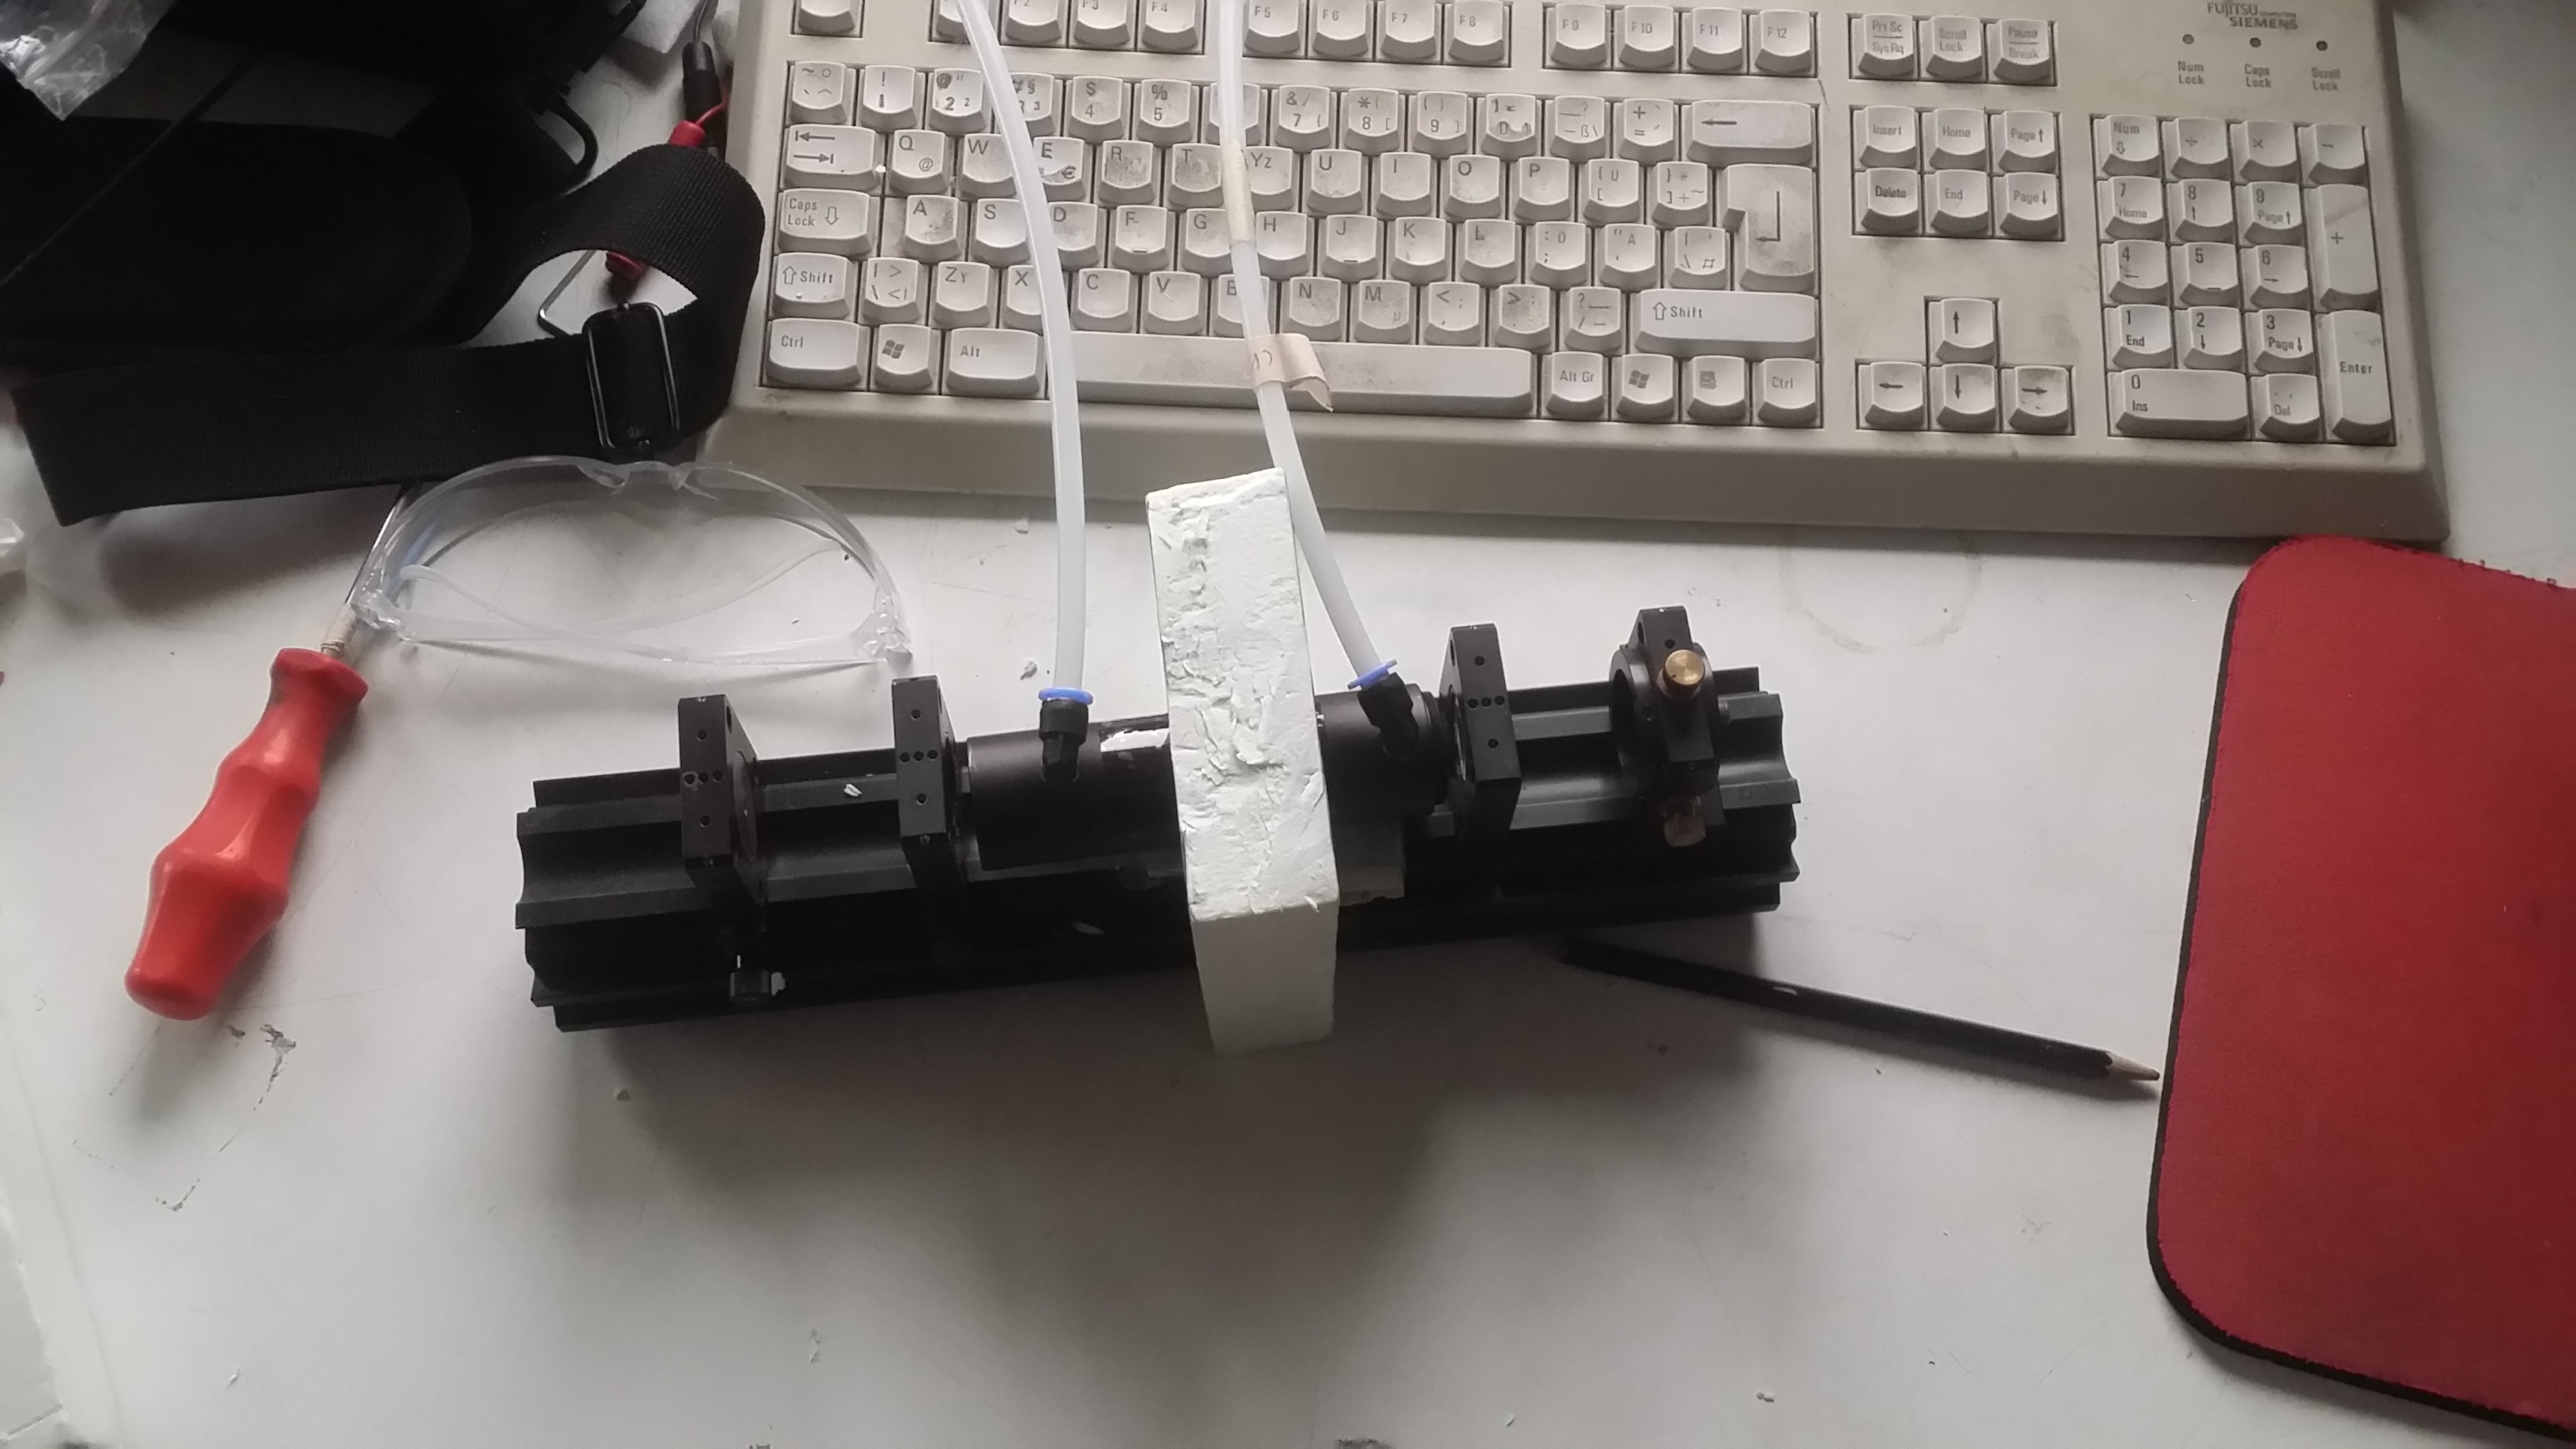
\includegraphics[width=0.7\textwidth]{images/cuvette.jpg}
  \caption{Cuvette together with styrofoam mount on an optical
    rack. The outermost riders are the mounts for the optical
    fibers. The riders within consist of two collimators.}
  \label{fig:cuvette}
\end{figure}

\begin{figure}[htbp]
  \centering
  {
  \def\svgwidth{0.9\linewidth}
  %% Creator: Inkscape inkscape 0.91, www.inkscape.org
%% PDF/EPS/PS + LaTeX output extension by Johan Engelen, 2010
%% Accompanies image file 'setup.pdf_tex.pdf' (pdf, eps, ps)
%%
%% To include the image in your LaTeX document, write
%%   \input{<filename>.pdf_tex}
%%  instead of
%%   \includegraphics{<filename>.pdf}
%% To scale the image, write
%%   \def\svgwidth{<desired width>}
%%   \input{<filename>.pdf_tex}
%%  instead of
%%   \includegraphics[width=<desired width>]{<filename>.pdf}
%%
%% Images with a different path to the parent latex file can
%% be accessed with the `import' package (which may need to be
%% installed) using
%%   \usepackage{import}
%% in the preamble, and then including the image with
%%   \import{<path to file>}{<filename>.pdf_tex}
%% Alternatively, one can specify
%%   \graphicspath{{<path to file>/}}
%% 
%% For more information, please see info/svg-inkscape on CTAN:
%%   http://tug.ctan.org/tex-archive/info/svg-inkscape
%%
\begingroup%
  \makeatletter%
  \providecommand\color[2][]{%
    \errmessage{(Inkscape) Color is used for the text in Inkscape, but the package 'color.sty' is not loaded}%
    \renewcommand\color[2][]{}%
  }%
  \providecommand\transparent[1]{%
    \errmessage{(Inkscape) Transparency is used (non-zero) for the text in Inkscape, but the package 'transparent.sty' is not loaded}%
    \renewcommand\transparent[1]{}%
  }%
  \providecommand\rotatebox[2]{#2}%
  \ifx\svgwidth\undefined%
    \setlength{\unitlength}{1567.76523438bp}%
    \ifx\svgscale\undefined%
      \relax%
    \else%
      \setlength{\unitlength}{\unitlength * \real{\svgscale}}%
    \fi%
  \else%
    \setlength{\unitlength}{\svgwidth}%
  \fi%
  \global\let\svgwidth\undefined%
  \global\let\svgscale\undefined%
  \makeatother%
  \begin{picture}(1,0.56250002)%
    \put(0,0){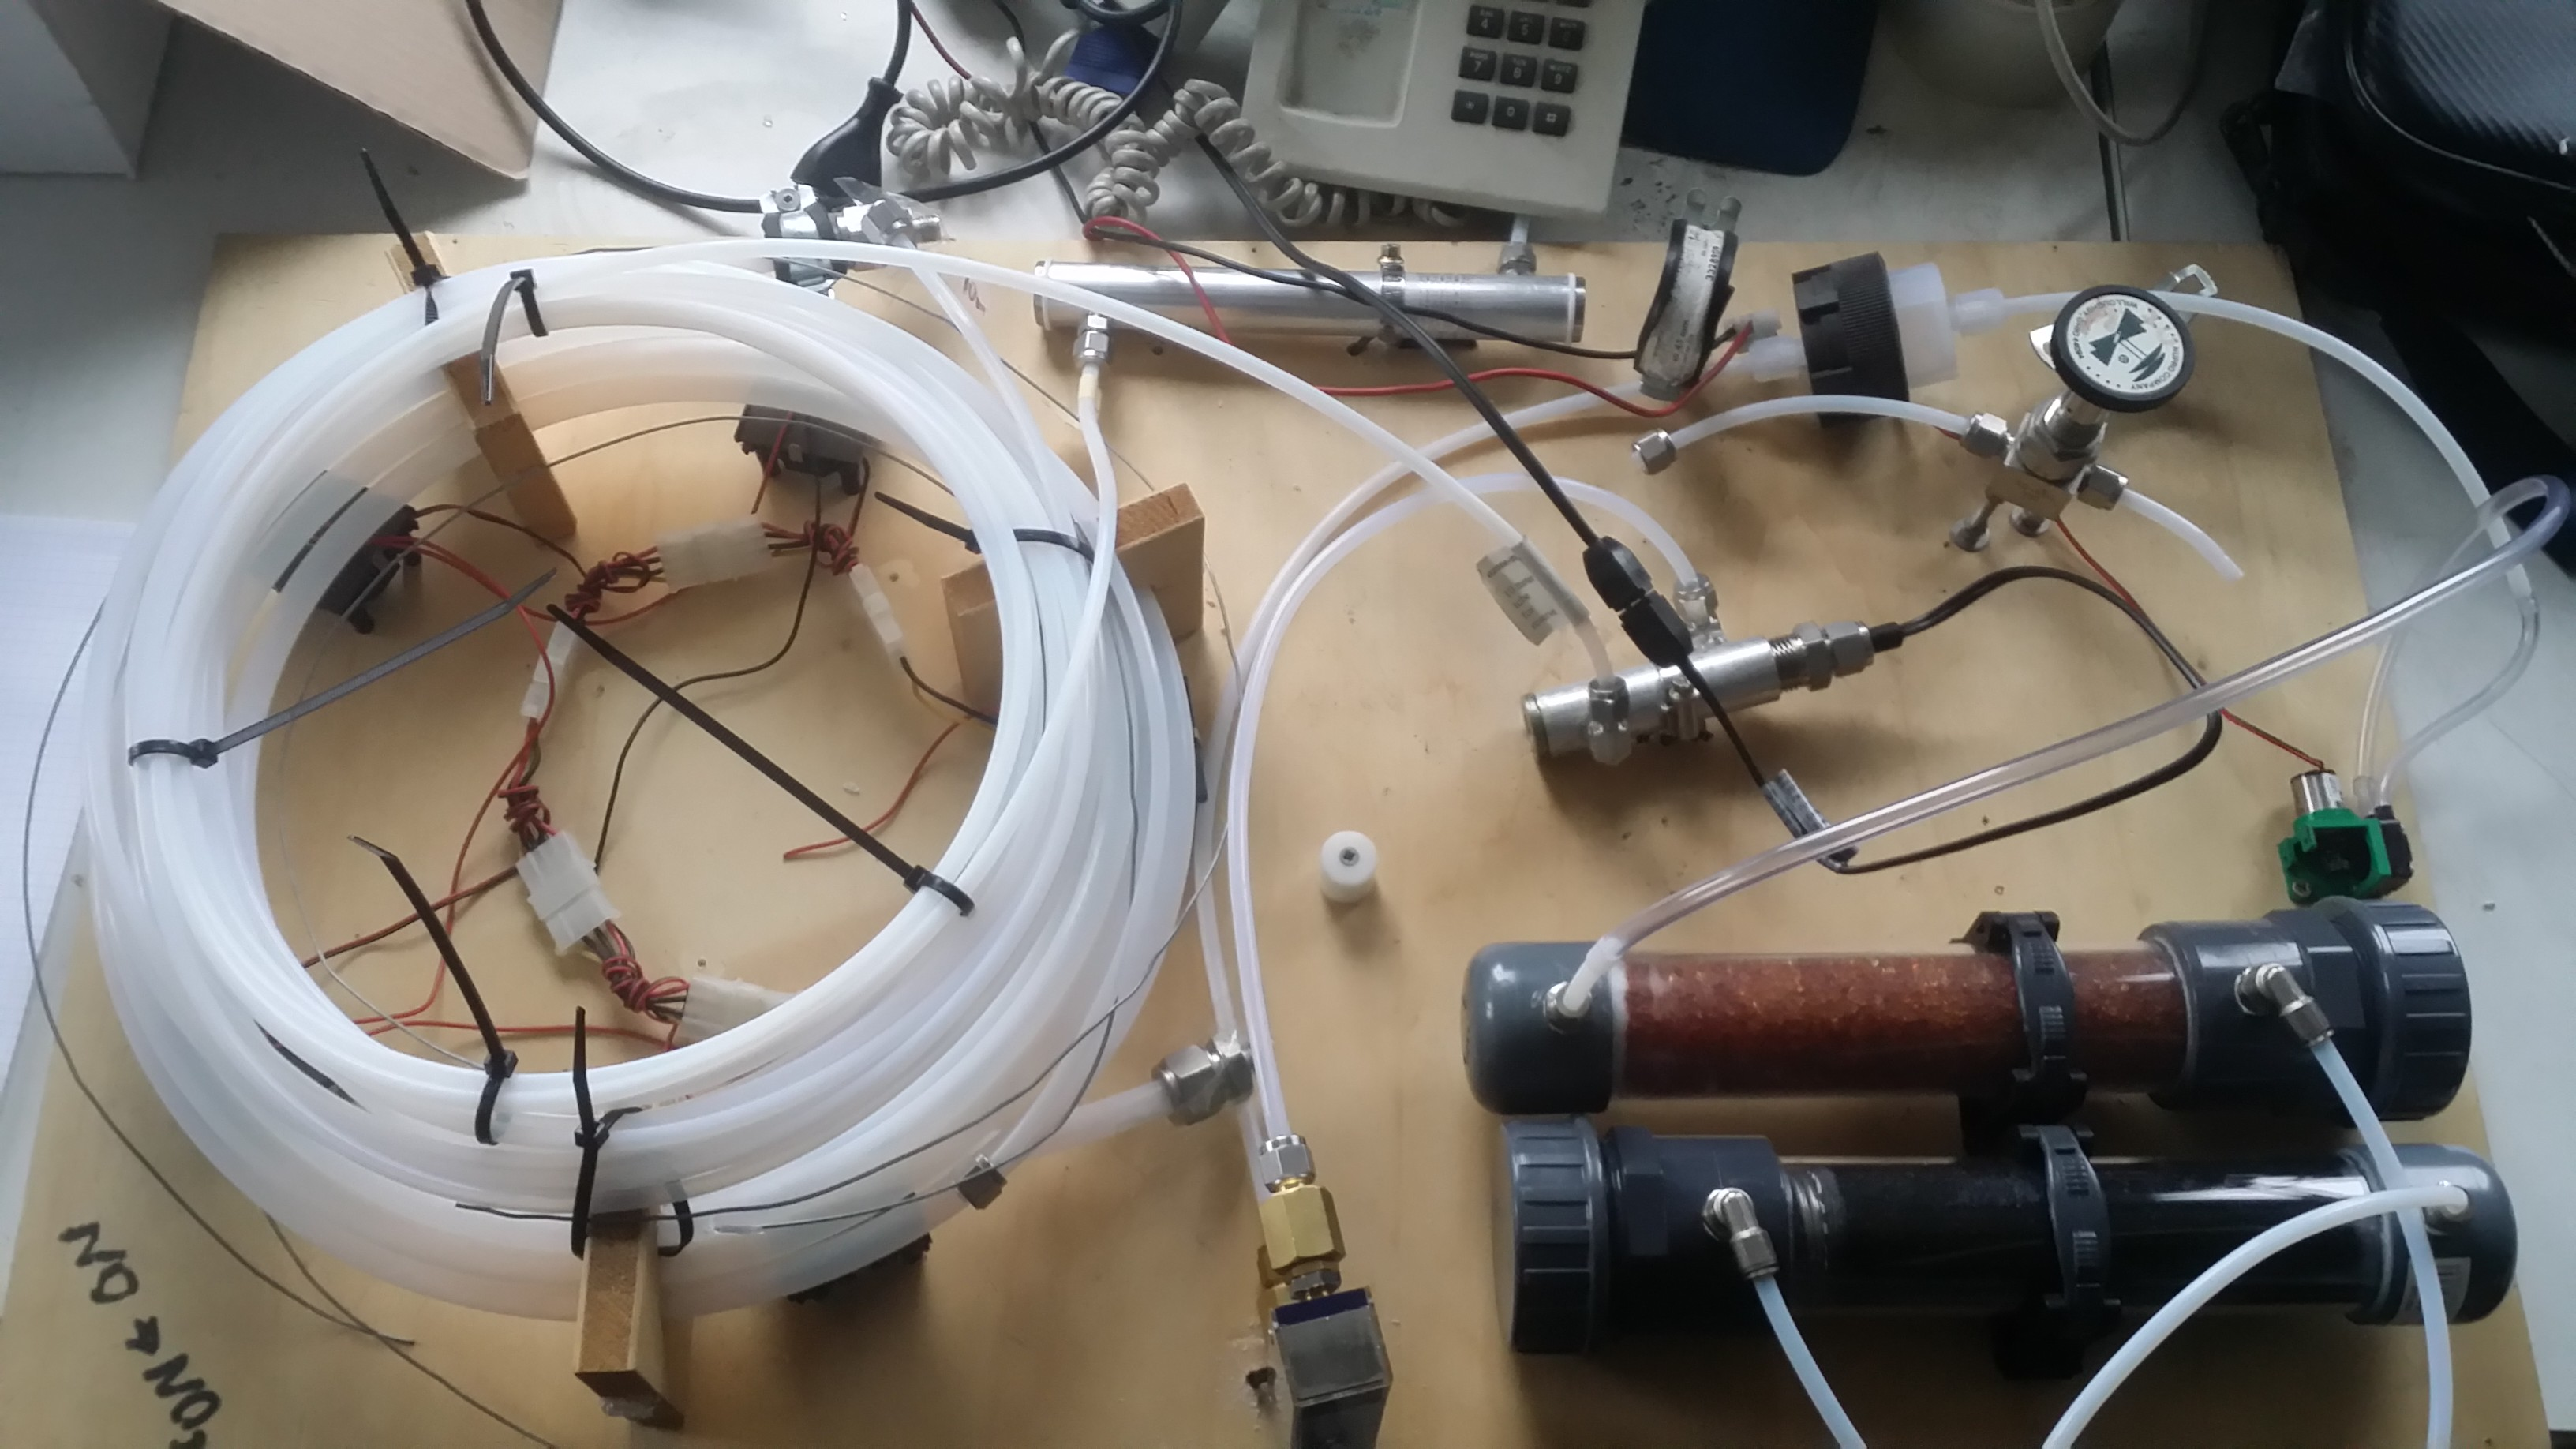
\includegraphics[width=\unitlength,page=1]{setup.pdf}}%
    \put(0.72339254,0.0272422){\color[rgb]{0,0,0}\makebox(0,0)[lb]{carbon filter}}%
    \put(0.68467052,0.20608212){\color[rgb]{0,0,0}\makebox(0,0)[lb]{\smash{silica gel}}}%
    \put(0.84485225,0.27636329){\color[rgb]{0,0,0}\makebox(0,0)[lb]{\smash{pump}}}%
    \put(0.66524548,0.47215208){\color[rgb]{0,0,0}\makebox(0,0)[lb]{\smash{particle filter}}}%
    \put(0.37854499,0.02340413){\color[rgb]{0,0,0}\makebox(0,0)[lb]{\smash{flowmeter}}}%
    \put(0.41093385,0.46876799){\color[rgb]{0,0,0}\makebox(0,0)[lb]{\smash{silica gel in tube}}}%
    \put(0.55474278,0.26558162){\color[rgb]{0,0,0}\makebox(0,0)[lb]{\smash{penray lamp in tube}}}%
    \put(0,0){\includegraphics[width=\unitlength,page=2]{setup.pdf}}%
    \put(1.00286136,0.04729665){\color[rgb]{0,0,0}\makebox(0,0)[lb]{\smash{lab air}}}%
    \put(0.59985726,0.5399915){\color[rgb]{0,0,0}\makebox(0,0)[lb]{\smash{ozone}}}%
    \put(0,0){\includegraphics[width=\unitlength,page=3]{setup.pdf}}%
  \end{picture}%
\endgroup%

%%% Local Variables:
%%% mode: latex
%%% TeX-master: "../Bachelor"
%%% End:

  }
  \phantom{h}\\
  \vspace{2cm}
  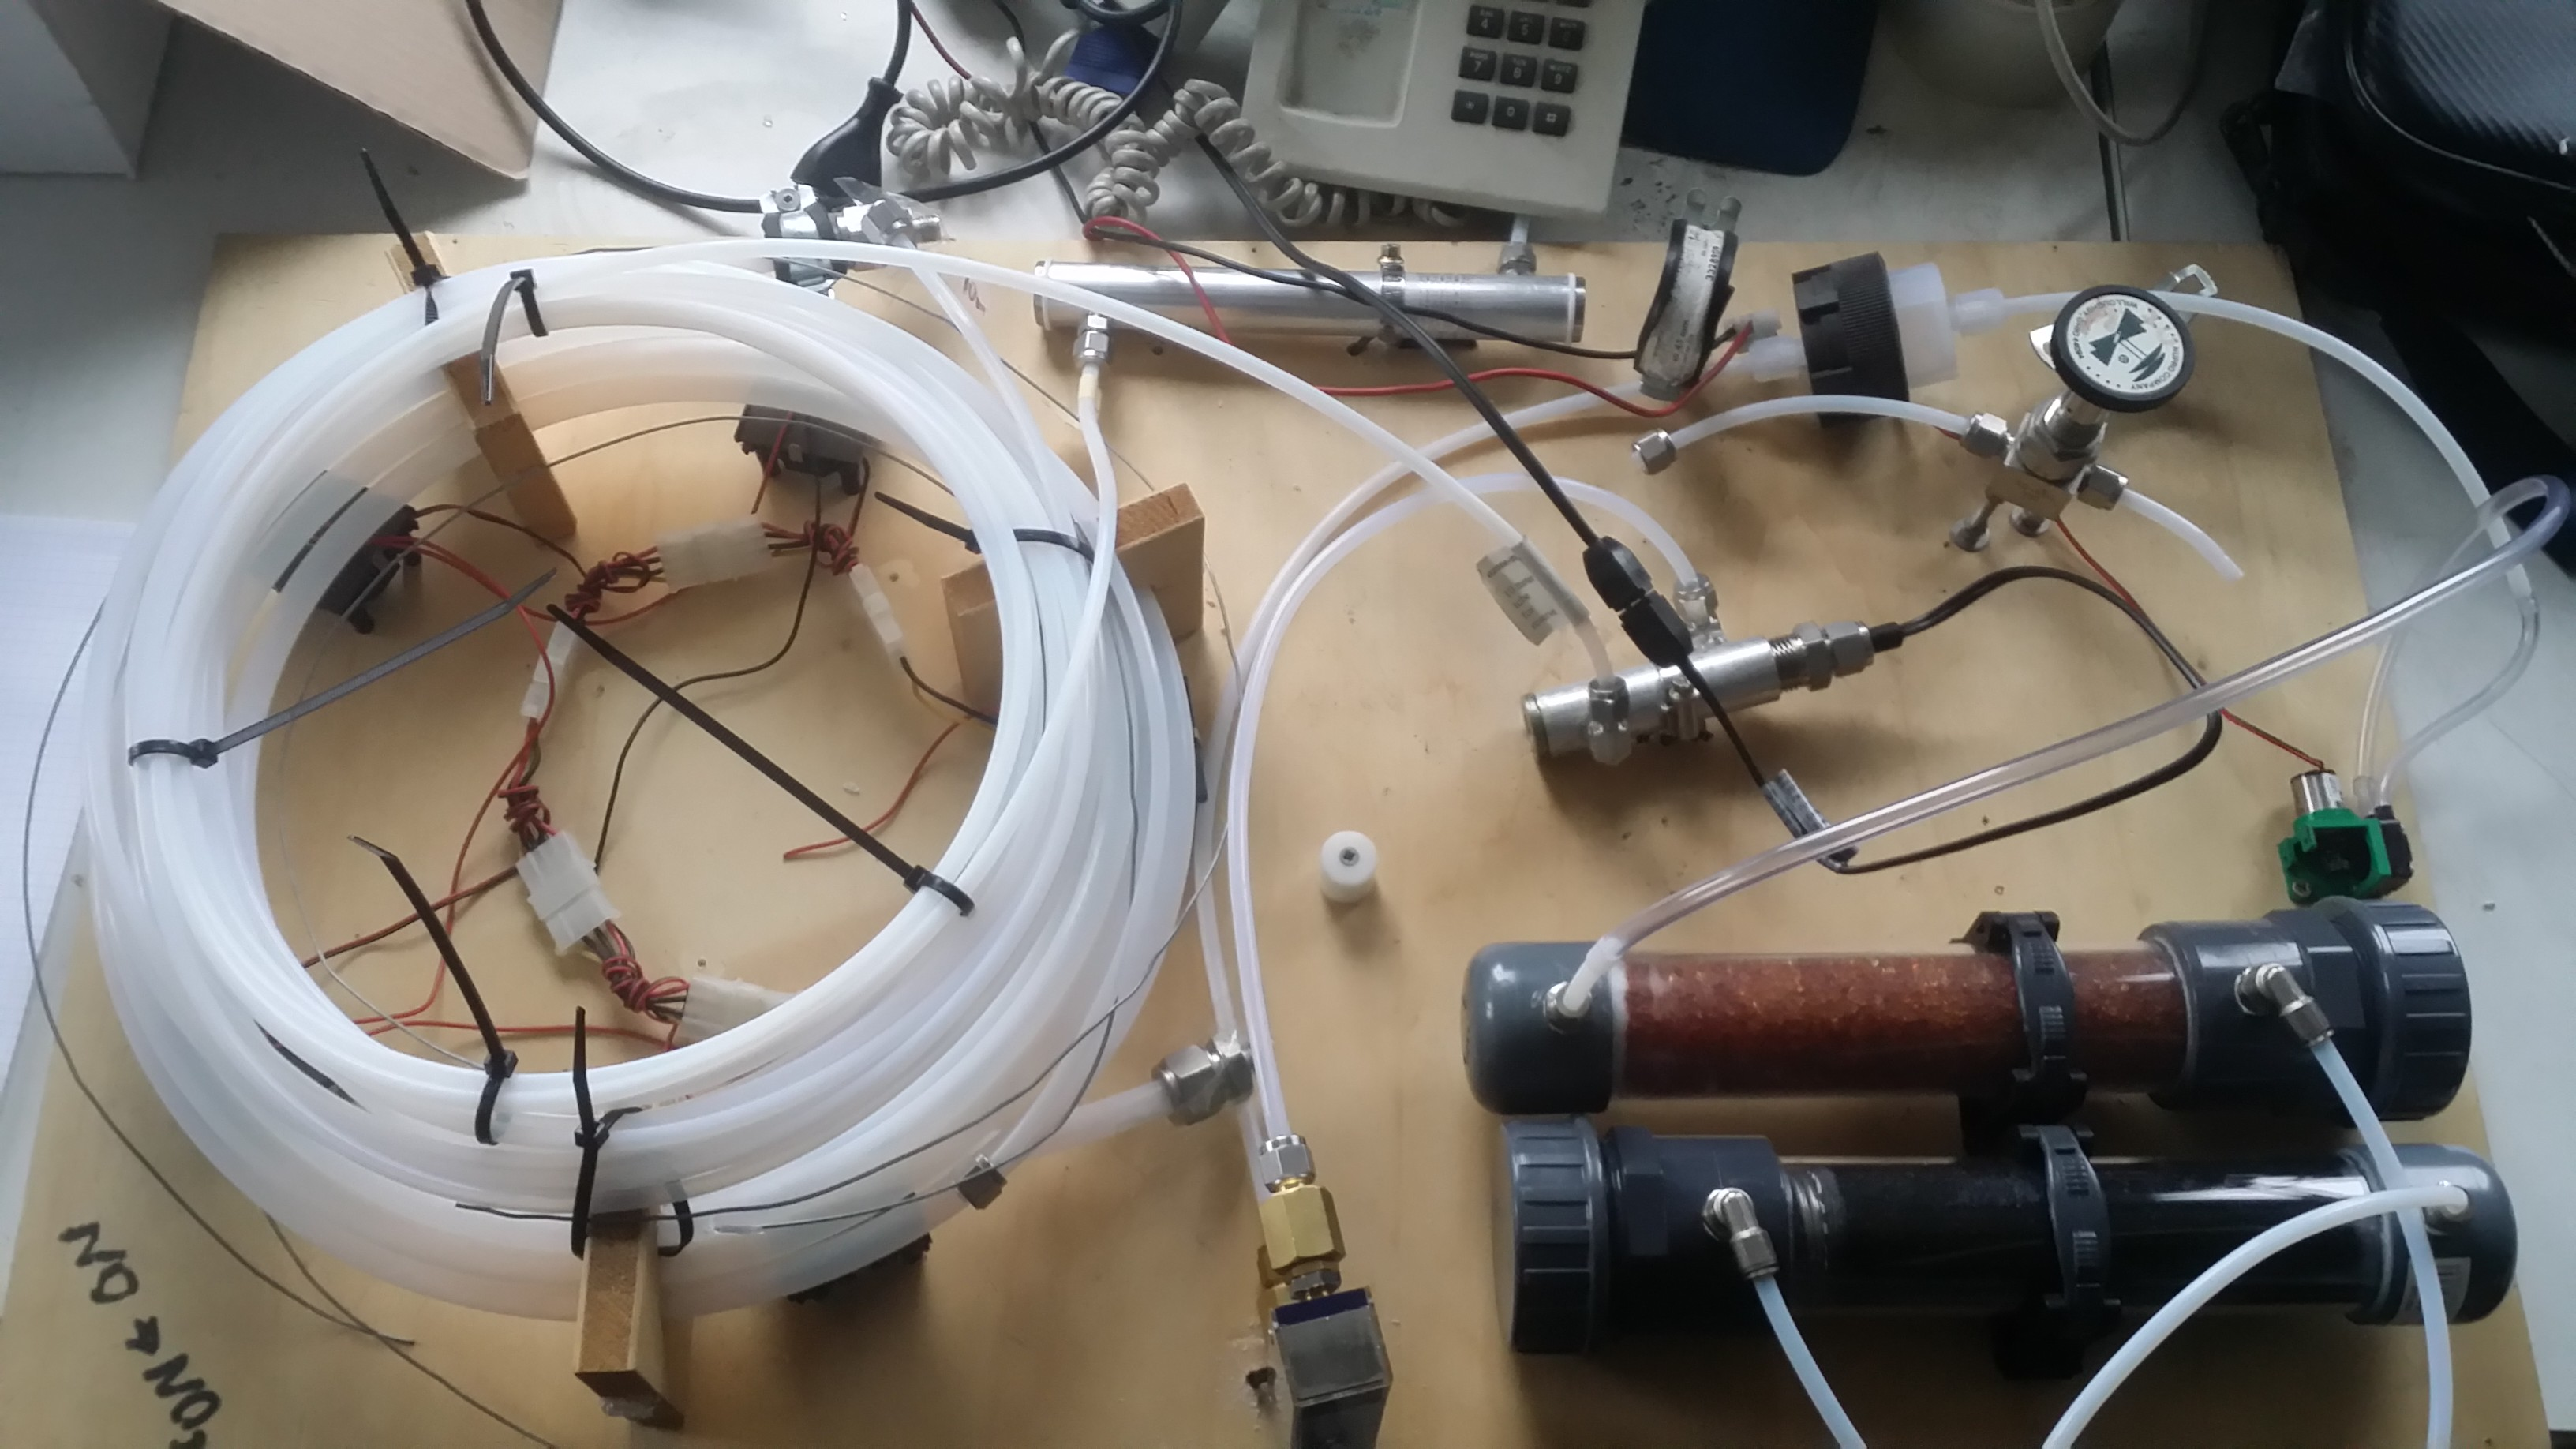
\includegraphics[width=0.9\linewidth]{setup.jpg}
  \caption{Ozone generator setup. Schematic and picture.}
  \label{fig:setup}
\end{figure}

The cuvette was entered into the ligthpath of a Longpath-DOAS
instrument (attached to an Amundsen telescope located at the height
laboratory at the IUP building). Since we expected rather high Ozone
concentrations, we forewent the advantage of a cavity enhanced
pathlength. The upside of this setup was that the instrument contains
a UV led emitting at a wavelength of $\lambda \approx
\SI{290}{\nano\meter}$. As mentioned in
Section~\ref{sec:theory-ozone}, Ozone has a strong absorption cross
section in this region, which allowed us to determine the
concentration very precisely.  The used spectrograph has 2048 channesl
and is calibrated to a wavelength region of \num{268} to
\SI{312}{\nano\meter}.

\subsection{Inclusion into a CE-DOAS instrument}
\label{sec:inclusion}

\begin{figure}[htbp]
  \centering
  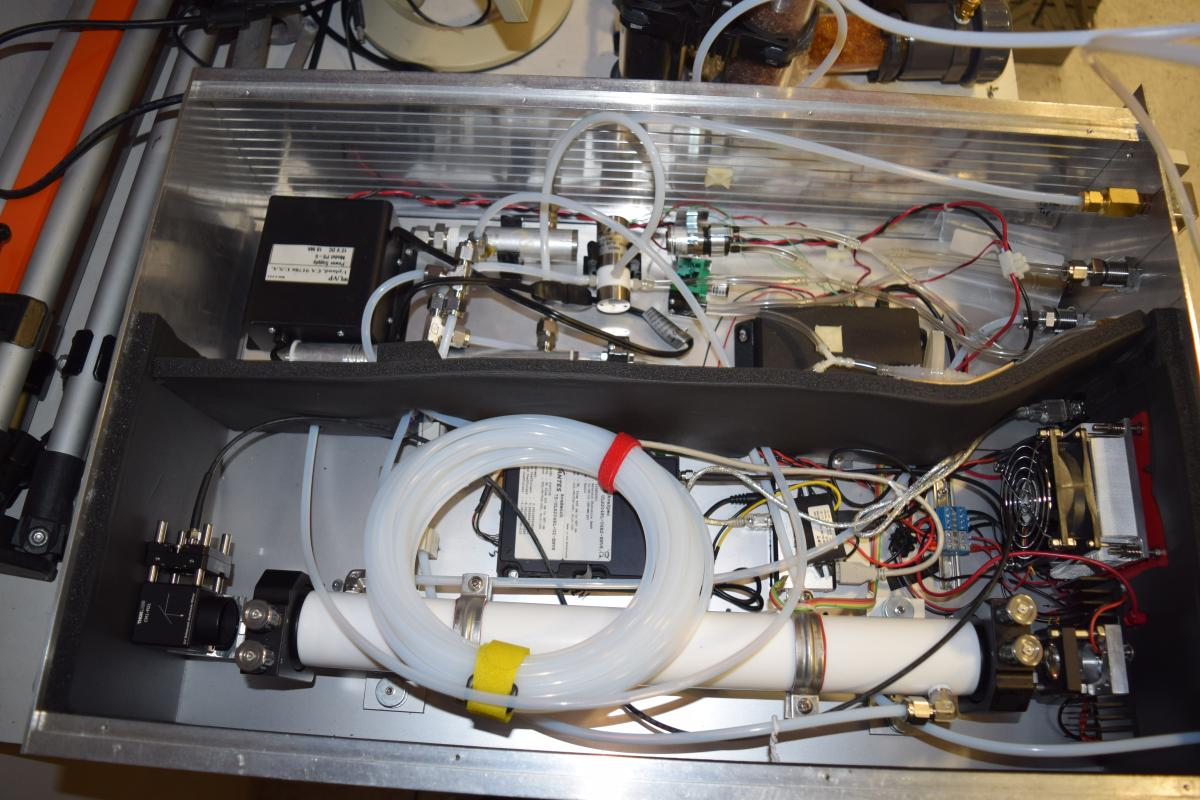
\includegraphics[width=0.8\textwidth]{images/envimes_up.jpg}
  \caption{EnviMeS CE-DOAS instrument with \ch{NO} to \ch{NO2}
    converter. On the upper left part the Pen-Ray lamp with
    powersupply can be seen. Below the powersupply partly covered by
    styrofoam is the additional Silica gel filter. In the lower half
    one can see the cavity with spectrometer and \SI{10}{\meter}
    reaction path rolled up.}
  \label{fig:envimes}
\end{figure}

\begin{figure}[htbp]
  \centering
  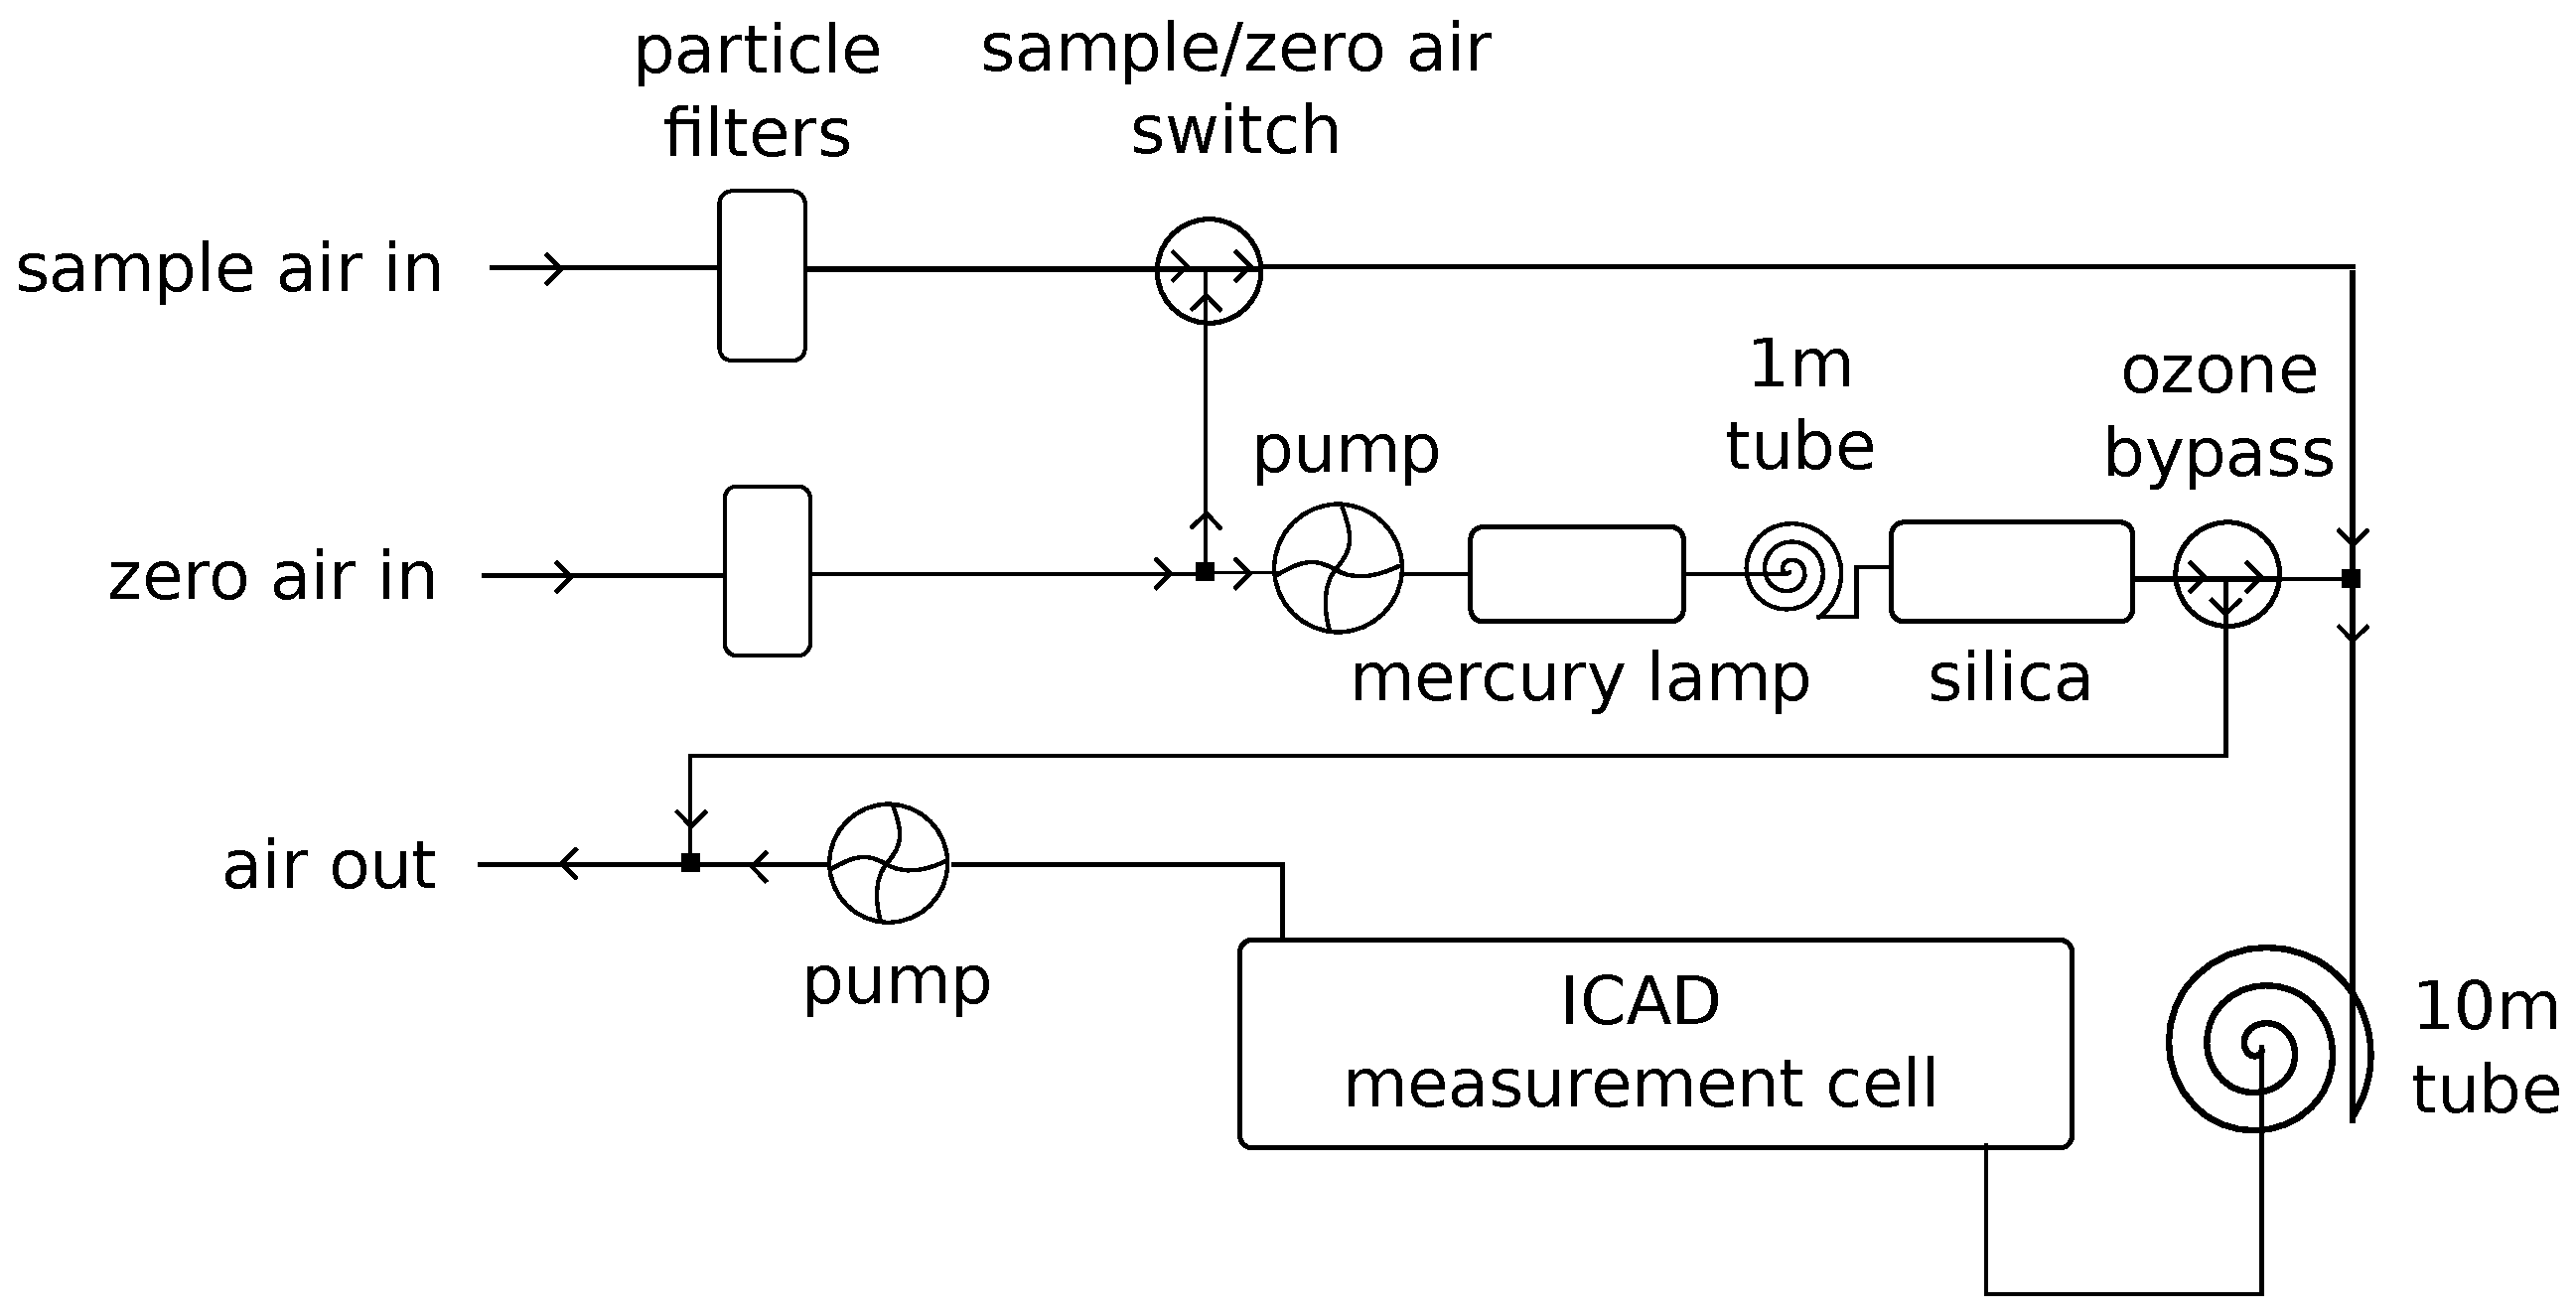
\includegraphics[width=0.8\textwidth]{images/envimes_setup.eps}
  \caption{Schematic of EnviMeS CE-DOAS instrument with \ch{NO} to
    \ch{NO2} converter.}
  \label{fig:envimes-schematic}
\end{figure}

After the above setup was tested the converter was added to an
existing CE-DOAS instrument (EnviMeS SN:2014002).  The instrument was
already supplied with an \ch{O3} generator, but lacked a Silica gel
filter, which was added. The inside of the instrument can be seen in
Figure~\ref{fig:envimes}. Since it is optimized for space, it is
difficult, if not impossible, to extract the setup from this
view. Therefore Figure~\ref{fig:envimes-schematic} contains a slightly
simplified schematic view of the instrument. The zero air input was
used to generate the Ozone, since it had already installed all the
necessary filters. After the Mercury lamp there was a \SI{1}{\meter}
reaction path before the silica filter followed. After that we had an
Ozone bypass valve, which was operated electromechanically and allowed
us to switch between an Ozone free and an Ozone enriched air flow in
the cavity. The sample air (with or without Ozone) passed a
\SI{10}{\meter} reaction path. In later experiments the length of the
reaction path was varied to measure the influence on the \ch{NO}
conversion (c.\,f.\ Sec.~\ref{sec:requirements} for the theory and
Sec.~\ref{sec:no} for measurements). The current for the Pen-Ray lamp
was fixed. The total flow $\Phi$ could be adapted, but was always set to
\SI{2}{\liter\per\minute}. The Ozone flow could be adapted (as in
Sec.~\ref{sec:ozone-setup}) from 0 to \SI{0.3}{\liter\per\minute}. The
lowest stable positive flow was \SI{0.03}{\liter\per\minute}. To
determine the Ozone production rate this flow was varied. When actual
\ch{NO} or \ch{NO_x} measurements were performed the flow was fixed to
\SI{0.03}{\liter\per\minute}.

The light source of the instrument was a led with maximum intensity at
$\lambda \approx \SI{444}{\nano\meter}$. The effective pathlength $L_0$ of
the cavity had a maximum at this wavelength of
\SI{1.3}{\kilo\meter}. A plot of the pathlength can be found in
Figure~\ref{fig:pathlength}. The spectrograph had \num{2048} channesl
and was calibrated to a wavelength region of \num{395} to
\SI{490}{\nano\meter}.

\begin{figure}[htbp]
  \centering
  %\includegraphics[width=0.7\textwidth]{L0.png}
  % GNUPLOT: LaTeX picture with Postscript
\begingroup
  \makeatletter
  \providecommand\color[2][]{%
    \GenericError{(gnuplot) \space\space\space\@spaces}{%
      Package color not loaded in conjunction with
      terminal option `colourtext'%
    }{See the gnuplot documentation for explanation.%
    }{Either use 'blacktext' in gnuplot or load the package
      color.sty in LaTeX.}%
    \renewcommand\color[2][]{}%
  }%
  \providecommand\includegraphics[2][]{%
    \GenericError{(gnuplot) \space\space\space\@spaces}{%
      Package graphicx or graphics not loaded%
    }{See the gnuplot documentation for explanation.%
    }{The gnuplot epslatex terminal needs graphicx.sty or graphics.sty.}%
    \renewcommand\includegraphics[2][]{}%
  }%
  \providecommand\rotatebox[2]{#2}%
  \@ifundefined{ifGPcolor}{%
    \newif\ifGPcolor
    \GPcolorfalse
  }{}%
  \@ifundefined{ifGPblacktext}{%
    \newif\ifGPblacktext
    \GPblacktexttrue
  }{}%
  % define a \g@addto@macro without @ in the name:
  \let\gplgaddtomacro\g@addto@macro
  % define empty templates for all commands taking text:
  \gdef\gplbacktext{}%
  \gdef\gplfronttext{}%
  \makeatother
  \ifGPblacktext
    % no textcolor at all
    \def\colorrgb#1{}%
    \def\colorgray#1{}%
  \else
    % gray or color?
    \ifGPcolor
      \def\colorrgb#1{\color[rgb]{#1}}%
      \def\colorgray#1{\color[gray]{#1}}%
      \expandafter\def\csname LTw\endcsname{\color{white}}%
      \expandafter\def\csname LTb\endcsname{\color{black}}%
      \expandafter\def\csname LTa\endcsname{\color{black}}%
      \expandafter\def\csname LT0\endcsname{\color[rgb]{1,0,0}}%
      \expandafter\def\csname LT1\endcsname{\color[rgb]{0,1,0}}%
      \expandafter\def\csname LT2\endcsname{\color[rgb]{0,0,1}}%
      \expandafter\def\csname LT3\endcsname{\color[rgb]{1,0,1}}%
      \expandafter\def\csname LT4\endcsname{\color[rgb]{0,1,1}}%
      \expandafter\def\csname LT5\endcsname{\color[rgb]{1,1,0}}%
      \expandafter\def\csname LT6\endcsname{\color[rgb]{0,0,0}}%
      \expandafter\def\csname LT7\endcsname{\color[rgb]{1,0.3,0}}%
      \expandafter\def\csname LT8\endcsname{\color[rgb]{0.5,0.5,0.5}}%
    \else
      % gray
      \def\colorrgb#1{\color{black}}%
      \def\colorgray#1{\color[gray]{#1}}%
      \expandafter\def\csname LTw\endcsname{\color{white}}%
      \expandafter\def\csname LTb\endcsname{\color{black}}%
      \expandafter\def\csname LTa\endcsname{\color{black}}%
      \expandafter\def\csname LT0\endcsname{\color{black}}%
      \expandafter\def\csname LT1\endcsname{\color{black}}%
      \expandafter\def\csname LT2\endcsname{\color{black}}%
      \expandafter\def\csname LT3\endcsname{\color{black}}%
      \expandafter\def\csname LT4\endcsname{\color{black}}%
      \expandafter\def\csname LT5\endcsname{\color{black}}%
      \expandafter\def\csname LT6\endcsname{\color{black}}%
      \expandafter\def\csname LT7\endcsname{\color{black}}%
      \expandafter\def\csname LT8\endcsname{\color{black}}%
    \fi
  \fi
    \setlength{\unitlength}{0.0500bp}%
    \ifx\gptboxheight\undefined%
      \newlength{\gptboxheight}%
      \newlength{\gptboxwidth}%
      \newsavebox{\gptboxtext}%
    \fi%
    \setlength{\fboxrule}{0.5pt}%
    \setlength{\fboxsep}{1pt}%
\begin{picture}(7776.00,4320.00)%
    \gplgaddtomacro\gplbacktext{%
      \csname LTb\endcsname%
      \put(946,704){\makebox(0,0)[r]{\strut{}$-0.2$}}%
      \put(946,1123){\makebox(0,0)[r]{\strut{}$0$}}%
      \put(946,1542){\makebox(0,0)[r]{\strut{}$0.2$}}%
      \put(946,1961){\makebox(0,0)[r]{\strut{}$0.4$}}%
      \put(946,2380){\makebox(0,0)[r]{\strut{}$0.6$}}%
      \put(946,2798){\makebox(0,0)[r]{\strut{}$0.8$}}%
      \put(946,3217){\makebox(0,0)[r]{\strut{}$1$}}%
      \put(946,3636){\makebox(0,0)[r]{\strut{}$1.2$}}%
      \put(946,4055){\makebox(0,0)[r]{\strut{}$1.4$}}%
      \put(1078,484){\makebox(0,0){\strut{}$390$}}%
      \put(1651,484){\makebox(0,0){\strut{}$400$}}%
      \put(2224,484){\makebox(0,0){\strut{}$410$}}%
      \put(2796,484){\makebox(0,0){\strut{}$420$}}%
      \put(3369,484){\makebox(0,0){\strut{}$430$}}%
      \put(3942,484){\makebox(0,0){\strut{}$440$}}%
      \put(4515,484){\makebox(0,0){\strut{}$450$}}%
      \put(5088,484){\makebox(0,0){\strut{}$460$}}%
      \put(5661,484){\makebox(0,0){\strut{}$470$}}%
      \put(6233,484){\makebox(0,0){\strut{}$480$}}%
      \put(6806,484){\makebox(0,0){\strut{}$490$}}%
      \put(7379,484){\makebox(0,0){\strut{}$500$}}%
    }%
    \gplgaddtomacro\gplfronttext{%
      \csname LTb\endcsname%
      \put(176,2379){\rotatebox{-270}{\makebox(0,0){\strut{}Pathlength [km]}}}%
      \put(4228,154){\makebox(0,0){\strut{}Wavelength [nm]}}%
    }%
    \gplbacktext
    \put(0,0){\includegraphics{../images/L0}}%
    \gplfronttext
  \end{picture}%
\endgroup

  \caption{Effective pathlength of the used EnviMeS CE-DOAS system.}
  \label{fig:pathlength}
\end{figure}


%%% Local Variables:
%%% mode: latex
%%% TeX-master: "../Bachelor"
%%% End:

\cleardoubleoddstandardpage{}

\section{Measurements}
\label{sec:measurements}

This section contains all the measurements conducted to characterize
and test our converter. To evaluate our measured spectra we used the
DOAS Intelligent System (DOASIS) software package~\cite{doasis} with
the ICAD evaluation script (v1.1) by M.\ Horbanski and the LP-DOAS
Data fitting script by D.\ Pöhler. All used post processing and
plotting scripts can be found under~\cite{scripts}.

%%% Local Variables:
%%% mode: latex
%%% TeX-master: "../Bachelor"
%%% End:

\subsection{Startup behaviour of the ozone generator}
\label{sec:ozone}

During these first experiments, I wanted to assure that the ozone
generator produces enough ozone. More precisely I was interested,
whether the ozone could penetrate the Silica gel and how long it would
take for it to succeed. In a last step I wanted to calibrate the relation
between the ozone production and the applied electrical current at the
mercury lamp.

\subsubsection{Setup}
\label{sec:ozone-setup}

The following experiments were all conducted using the setup described
in Section~\ref{sec:ozone-setup}. Since the cuvette had to be entered
in and removed from the lightpath manually, the time resolution had to
be reduced to \SI{5}{\minute}. In a first step I measured the startup
\ch{O3} transmission through the silica gel filter after a one week
stop of the generator. Secondly, I researched the startup time
necessary after shorter stops. Lastly, I noted the influence of the
lamp current on the ozone concentration. Using this setup it was
impossible to measure the generator's \ch{NO2} productoin. Since the
concentration should be around the \ch{NO_x} concentration in ambient
lab air, it should be no more than a few \si{ppb}. This is far below
the detection limit of a `longpath' DOAS instrument with a pathlength
of \SI{8.6}{\centi\meter} and a LED peak at $\lambda \approx
\SI{290}{\nano\meter}$.

\subsubsection{Results}
\label{sec:ozone-results}

As a zeroth, qualitative experiment I turned on the generator
and succeeded in perceiving an ozone signal. After that I shut down the generator
for one week. The startup behaviour afterwards can be seen in
Figuer~\ref{fig:long-stop}. It shows that the generator takes about
\SI{35}{\minute} before it reaches its stable plateau of around
\SI{250}{ppb} ozone. During this experiment the flow was constantly
set to $\Phi_{\ch{O_3}} = \SI{0.03}{\liter\per\minute}$. It stands to
argue that the startup time could be shortened by increasing the flow,
however, as shall be seen shortly, if the
generator is used regularly, this procedure seems unnecessary.

\begin{figure}[htbp]
  \centering
  % GNUPLOT: LaTeX picture with Postscript
\begingroup
  \makeatletter
  \providecommand\color[2][]{%
    \GenericError{(gnuplot) \space\space\space\@spaces}{%
      Package color not loaded in conjunction with
      terminal option `colourtext'%
    }{See the gnuplot documentation for explanation.%
    }{Either use 'blacktext' in gnuplot or load the package
      color.sty in LaTeX.}%
    \renewcommand\color[2][]{}%
  }%
  \providecommand\includegraphics[2][]{%
    \GenericError{(gnuplot) \space\space\space\@spaces}{%
      Package graphicx or graphics not loaded%
    }{See the gnuplot documentation for explanation.%
    }{The gnuplot epslatex terminal needs graphicx.sty or graphics.sty.}%
    \renewcommand\includegraphics[2][]{}%
  }%
  \providecommand\rotatebox[2]{#2}%
  \@ifundefined{ifGPcolor}{%
    \newif\ifGPcolor
    \GPcolorfalse
  }{}%
  \@ifundefined{ifGPblacktext}{%
    \newif\ifGPblacktext
    \GPblacktexttrue
  }{}%
  % define a \g@addto@macro without @ in the name:
  \let\gplgaddtomacro\g@addto@macro
  % define empty templates for all commands taking text:
  \gdef\gplbacktext{}%
  \gdef\gplfronttext{}%
  \makeatother
  \ifGPblacktext
    % no textcolor at all
    \def\colorrgb#1{}%
    \def\colorgray#1{}%
  \else
    % gray or color?
    \ifGPcolor
      \def\colorrgb#1{\color[rgb]{#1}}%
      \def\colorgray#1{\color[gray]{#1}}%
      \expandafter\def\csname LTw\endcsname{\color{white}}%
      \expandafter\def\csname LTb\endcsname{\color{black}}%
      \expandafter\def\csname LTa\endcsname{\color{black}}%
      \expandafter\def\csname LT0\endcsname{\color[rgb]{1,0,0}}%
      \expandafter\def\csname LT1\endcsname{\color[rgb]{0,1,0}}%
      \expandafter\def\csname LT2\endcsname{\color[rgb]{0,0,1}}%
      \expandafter\def\csname LT3\endcsname{\color[rgb]{1,0,1}}%
      \expandafter\def\csname LT4\endcsname{\color[rgb]{0,1,1}}%
      \expandafter\def\csname LT5\endcsname{\color[rgb]{1,1,0}}%
      \expandafter\def\csname LT6\endcsname{\color[rgb]{0,0,0}}%
      \expandafter\def\csname LT7\endcsname{\color[rgb]{1,0.3,0}}%
      \expandafter\def\csname LT8\endcsname{\color[rgb]{0.5,0.5,0.5}}%
    \else
      % gray
      \def\colorrgb#1{\color{black}}%
      \def\colorgray#1{\color[gray]{#1}}%
      \expandafter\def\csname LTw\endcsname{\color{white}}%
      \expandafter\def\csname LTb\endcsname{\color{black}}%
      \expandafter\def\csname LTa\endcsname{\color{black}}%
      \expandafter\def\csname LT0\endcsname{\color{black}}%
      \expandafter\def\csname LT1\endcsname{\color{black}}%
      \expandafter\def\csname LT2\endcsname{\color{black}}%
      \expandafter\def\csname LT3\endcsname{\color{black}}%
      \expandafter\def\csname LT4\endcsname{\color{black}}%
      \expandafter\def\csname LT5\endcsname{\color{black}}%
      \expandafter\def\csname LT6\endcsname{\color{black}}%
      \expandafter\def\csname LT7\endcsname{\color{black}}%
      \expandafter\def\csname LT8\endcsname{\color{black}}%
    \fi
  \fi
    \setlength{\unitlength}{0.0500bp}%
    \ifx\gptboxheight\undefined%
      \newlength{\gptboxheight}%
      \newlength{\gptboxwidth}%
      \newsavebox{\gptboxtext}%
    \fi%
    \setlength{\fboxrule}{0.5pt}%
    \setlength{\fboxsep}{1pt}%
\begin{picture}(7776.00,3888.00)%
    \gplgaddtomacro\gplbacktext{%
      \csname LTb\endcsname%
      \put(814,704){\makebox(0,0)[r]{\strut{}$0$}}%
      \put(814,1191){\makebox(0,0)[r]{\strut{}$50$}}%
      \put(814,1677){\makebox(0,0)[r]{\strut{}$100$}}%
      \put(814,2164){\makebox(0,0)[r]{\strut{}$150$}}%
      \put(814,2650){\makebox(0,0)[r]{\strut{}$200$}}%
      \put(814,3137){\makebox(0,0)[r]{\strut{}$250$}}%
      \put(814,3623){\makebox(0,0)[r]{\strut{}$300$}}%
      \put(946,484){\makebox(0,0){\strut{}$0$}}%
      \put(2233,484){\makebox(0,0){\strut{}$0.5$}}%
      \put(3519,484){\makebox(0,0){\strut{}$1$}}%
      \put(4806,484){\makebox(0,0){\strut{}$1.5$}}%
      \put(6092,484){\makebox(0,0){\strut{}$2$}}%
      \put(7379,484){\makebox(0,0){\strut{}$2.5$}}%
    }%
    \gplgaddtomacro\gplfronttext{%
      \csname LTb\endcsname%
      \put(176,2163){\rotatebox{-270}{\makebox(0,0){\strut{}Concentration [ppm]}}}%
      \put(4162,154){\makebox(0,0){\strut{}Time [h]}}%
    }%
    \gplbacktext
    \put(0,0){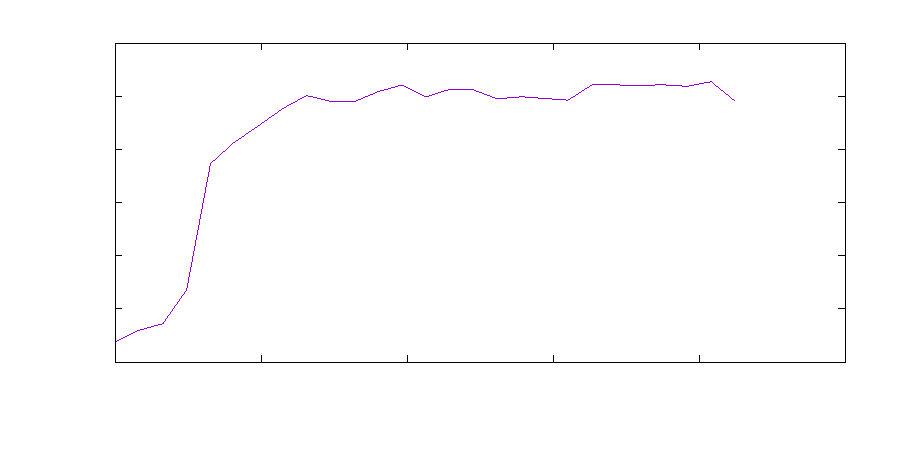
\includegraphics{../images/startup}}%
    \gplfronttext
  \end{picture}%
\endgroup

  \caption{Evolution of ozone after a long full stop of the
    generator.}
  \label{fig:long-stop}
\end{figure}
\begin{figure}[htbp]
  \centering
  % GNUPLOT: LaTeX picture with Postscript
\begingroup
  \makeatletter
  \providecommand\color[2][]{%
    \GenericError{(gnuplot) \space\space\space\@spaces}{%
      Package color not loaded in conjunction with
      terminal option `colourtext'%
    }{See the gnuplot documentation for explanation.%
    }{Either use 'blacktext' in gnuplot or load the package
      color.sty in LaTeX.}%
    \renewcommand\color[2][]{}%
  }%
  \providecommand\includegraphics[2][]{%
    \GenericError{(gnuplot) \space\space\space\@spaces}{%
      Package graphicx or graphics not loaded%
    }{See the gnuplot documentation for explanation.%
    }{The gnuplot epslatex terminal needs graphicx.sty or graphics.sty.}%
    \renewcommand\includegraphics[2][]{}%
  }%
  \providecommand\rotatebox[2]{#2}%
  \@ifundefined{ifGPcolor}{%
    \newif\ifGPcolor
    \GPcolorfalse
  }{}%
  \@ifundefined{ifGPblacktext}{%
    \newif\ifGPblacktext
    \GPblacktexttrue
  }{}%
  % define a \g@addto@macro without @ in the name:
  \let\gplgaddtomacro\g@addto@macro
  % define empty templates for all commands taking text:
  \gdef\gplbacktext{}%
  \gdef\gplfronttext{}%
  \makeatother
  \ifGPblacktext
    % no textcolor at all
    \def\colorrgb#1{}%
    \def\colorgray#1{}%
  \else
    % gray or color?
    \ifGPcolor
      \def\colorrgb#1{\color[rgb]{#1}}%
      \def\colorgray#1{\color[gray]{#1}}%
      \expandafter\def\csname LTw\endcsname{\color{white}}%
      \expandafter\def\csname LTb\endcsname{\color{black}}%
      \expandafter\def\csname LTa\endcsname{\color{black}}%
      \expandafter\def\csname LT0\endcsname{\color[rgb]{1,0,0}}%
      \expandafter\def\csname LT1\endcsname{\color[rgb]{0,1,0}}%
      \expandafter\def\csname LT2\endcsname{\color[rgb]{0,0,1}}%
      \expandafter\def\csname LT3\endcsname{\color[rgb]{1,0,1}}%
      \expandafter\def\csname LT4\endcsname{\color[rgb]{0,1,1}}%
      \expandafter\def\csname LT5\endcsname{\color[rgb]{1,1,0}}%
      \expandafter\def\csname LT6\endcsname{\color[rgb]{0,0,0}}%
      \expandafter\def\csname LT7\endcsname{\color[rgb]{1,0.3,0}}%
      \expandafter\def\csname LT8\endcsname{\color[rgb]{0.5,0.5,0.5}}%
    \else
      % gray
      \def\colorrgb#1{\color{black}}%
      \def\colorgray#1{\color[gray]{#1}}%
      \expandafter\def\csname LTw\endcsname{\color{white}}%
      \expandafter\def\csname LTb\endcsname{\color{black}}%
      \expandafter\def\csname LTa\endcsname{\color{black}}%
      \expandafter\def\csname LT0\endcsname{\color{black}}%
      \expandafter\def\csname LT1\endcsname{\color{black}}%
      \expandafter\def\csname LT2\endcsname{\color{black}}%
      \expandafter\def\csname LT3\endcsname{\color{black}}%
      \expandafter\def\csname LT4\endcsname{\color{black}}%
      \expandafter\def\csname LT5\endcsname{\color{black}}%
      \expandafter\def\csname LT6\endcsname{\color{black}}%
      \expandafter\def\csname LT7\endcsname{\color{black}}%
      \expandafter\def\csname LT8\endcsname{\color{black}}%
    \fi
  \fi
    \setlength{\unitlength}{0.0500bp}%
    \ifx\gptboxheight\undefined%
      \newlength{\gptboxheight}%
      \newlength{\gptboxwidth}%
      \newsavebox{\gptboxtext}%
    \fi%
    \setlength{\fboxrule}{0.5pt}%
    \setlength{\fboxsep}{1pt}%
\begin{picture}(4030.00,4030.00)%
    \gplgaddtomacro\gplbacktext{%
      \csname LTb\endcsname%
      \put(814,704){\makebox(0,0)[r]{\strut{}$80$}}%
      \put(814,1141){\makebox(0,0)[r]{\strut{}$100$}}%
      \put(814,1579){\makebox(0,0)[r]{\strut{}$120$}}%
      \put(814,2016){\makebox(0,0)[r]{\strut{}$140$}}%
      \put(814,2453){\makebox(0,0)[r]{\strut{}$160$}}%
      \put(814,2890){\makebox(0,0)[r]{\strut{}$180$}}%
      \put(814,3328){\makebox(0,0)[r]{\strut{}$200$}}%
      \put(814,3765){\makebox(0,0)[r]{\strut{}$220$}}%
      \put(946,484){\makebox(0,0){\strut{}$0$}}%
      \put(1483,484){\makebox(0,0){\strut{}$2$}}%
      \put(2021,484){\makebox(0,0){\strut{}$4$}}%
      \put(2558,484){\makebox(0,0){\strut{}$6$}}%
      \put(3096,484){\makebox(0,0){\strut{}$8$}}%
      \put(3633,484){\makebox(0,0){\strut{}$10$}}%
    }%
    \gplgaddtomacro\gplfronttext{%
      \csname LTb\endcsname%
      \put(176,2234){\rotatebox{-270}{\makebox(0,0){\strut{}Concentration [ppm]}}}%
      \put(2289,154){\makebox(0,0){\strut{}Time [min]}}%
      \csname LTb\endcsname%
      \put(2646,1537){\makebox(-200,0){\nfrac{} 1/2 h}}%
      \csname LTb\endcsname%
      \put(2646,1317){\makebox(-100,0){1 h}}%
      \csname LTb\endcsname%
      \put(2646,1097){\makebox(-100,0){2 h}}%
      \csname LTb\endcsname%
      \put(2646,877){\makebox(-100,0){4 h}}%
    }%
    \gplbacktext
    \put(0,0){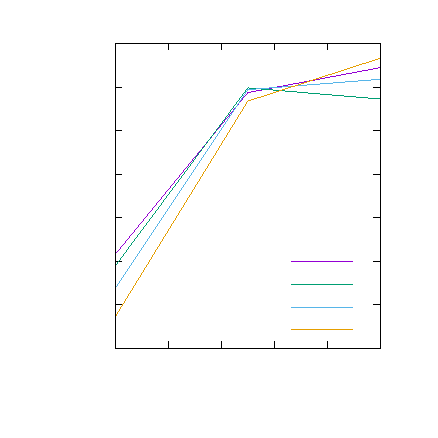
\includegraphics{../images/multi}}%
    \gplfronttext
  \end{picture}%
\endgroup

  \hfill
  % GNUPLOT: LaTeX picture with Postscript
\begingroup
  \makeatletter
  \providecommand\color[2][]{%
    \GenericError{(gnuplot) \space\space\space\@spaces}{%
      Package color not loaded in conjunction with
      terminal option `colourtext'%
    }{See the gnuplot documentation for explanation.%
    }{Either use 'blacktext' in gnuplot or load the package
      color.sty in LaTeX.}%
    \renewcommand\color[2][]{}%
  }%
  \providecommand\includegraphics[2][]{%
    \GenericError{(gnuplot) \space\space\space\@spaces}{%
      Package graphicx or graphics not loaded%
    }{See the gnuplot documentation for explanation.%
    }{The gnuplot epslatex terminal needs graphicx.sty or graphics.sty.}%
    \renewcommand\includegraphics[2][]{}%
  }%
  \providecommand\rotatebox[2]{#2}%
  \@ifundefined{ifGPcolor}{%
    \newif\ifGPcolor
    \GPcolorfalse
  }{}%
  \@ifundefined{ifGPblacktext}{%
    \newif\ifGPblacktext
    \GPblacktexttrue
  }{}%
  % define a \g@addto@macro without @ in the name:
  \let\gplgaddtomacro\g@addto@macro
  % define empty templates for all commands taking text:
  \gdef\gplbacktext{}%
  \gdef\gplfronttext{}%
  \makeatother
  \ifGPblacktext
    % no textcolor at all
    \def\colorrgb#1{}%
    \def\colorgray#1{}%
  \else
    % gray or color?
    \ifGPcolor
      \def\colorrgb#1{\color[rgb]{#1}}%
      \def\colorgray#1{\color[gray]{#1}}%
      \expandafter\def\csname LTw\endcsname{\color{white}}%
      \expandafter\def\csname LTb\endcsname{\color{black}}%
      \expandafter\def\csname LTa\endcsname{\color{black}}%
      \expandafter\def\csname LT0\endcsname{\color[rgb]{1,0,0}}%
      \expandafter\def\csname LT1\endcsname{\color[rgb]{0,1,0}}%
      \expandafter\def\csname LT2\endcsname{\color[rgb]{0,0,1}}%
      \expandafter\def\csname LT3\endcsname{\color[rgb]{1,0,1}}%
      \expandafter\def\csname LT4\endcsname{\color[rgb]{0,1,1}}%
      \expandafter\def\csname LT5\endcsname{\color[rgb]{1,1,0}}%
      \expandafter\def\csname LT6\endcsname{\color[rgb]{0,0,0}}%
      \expandafter\def\csname LT7\endcsname{\color[rgb]{1,0.3,0}}%
      \expandafter\def\csname LT8\endcsname{\color[rgb]{0.5,0.5,0.5}}%
    \else
      % gray
      \def\colorrgb#1{\color{black}}%
      \def\colorgray#1{\color[gray]{#1}}%
      \expandafter\def\csname LTw\endcsname{\color{white}}%
      \expandafter\def\csname LTb\endcsname{\color{black}}%
      \expandafter\def\csname LTa\endcsname{\color{black}}%
      \expandafter\def\csname LT0\endcsname{\color{black}}%
      \expandafter\def\csname LT1\endcsname{\color{black}}%
      \expandafter\def\csname LT2\endcsname{\color{black}}%
      \expandafter\def\csname LT3\endcsname{\color{black}}%
      \expandafter\def\csname LT4\endcsname{\color{black}}%
      \expandafter\def\csname LT5\endcsname{\color{black}}%
      \expandafter\def\csname LT6\endcsname{\color{black}}%
      \expandafter\def\csname LT7\endcsname{\color{black}}%
      \expandafter\def\csname LT8\endcsname{\color{black}}%
    \fi
  \fi
    \setlength{\unitlength}{0.0500bp}%
    \ifx\gptboxheight\undefined%
      \newlength{\gptboxheight}%
      \newlength{\gptboxwidth}%
      \newsavebox{\gptboxtext}%
    \fi%
    \setlength{\fboxrule}{0.5pt}%
    \setlength{\fboxsep}{1pt}%
\begin{picture}(4030.00,4030.00)%
    \gplgaddtomacro\gplbacktext{%
      \csname LTb\endcsname%
      \put(814,704){\makebox(0,0)[r]{\strut{}$200$}}%
      \put(814,1010){\makebox(0,0)[r]{\strut{}$220$}}%
      \put(814,1316){\makebox(0,0)[r]{\strut{}$240$}}%
      \put(814,1622){\makebox(0,0)[r]{\strut{}$260$}}%
      \put(814,1928){\makebox(0,0)[r]{\strut{}$280$}}%
      \put(814,2235){\makebox(0,0)[r]{\strut{}$300$}}%
      \put(814,2541){\makebox(0,0)[r]{\strut{}$320$}}%
      \put(814,2847){\makebox(0,0)[r]{\strut{}$340$}}%
      \put(814,3153){\makebox(0,0)[r]{\strut{}$360$}}%
      \put(814,3459){\makebox(0,0)[r]{\strut{}$380$}}%
      \put(814,3765){\makebox(0,0)[r]{\strut{}$400$}}%
      \put(946,484){\makebox(0,0){\strut{}$0$}}%
      \put(1245,484){\makebox(0,0){\strut{}$5$}}%
      \put(1543,484){\makebox(0,0){\strut{}$10$}}%
      \put(1842,484){\makebox(0,0){\strut{}$15$}}%
      \put(2140,484){\makebox(0,0){\strut{}$20$}}%
      \put(2439,484){\makebox(0,0){\strut{}$25$}}%
      \put(2737,484){\makebox(0,0){\strut{}$30$}}%
      \put(3036,484){\makebox(0,0){\strut{}$35$}}%
      \put(3334,484){\makebox(0,0){\strut{}$40$}}%
      \put(3633,484){\makebox(0,0){\strut{}$45$}}%
    }%
    \gplgaddtomacro\gplfronttext{%
      \csname LTb\endcsname%
      \put(176,2234){\rotatebox{-270}{\makebox(0,0){\strut{}Concentration [ppm]}}}%
      \put(2289,154){\makebox(0,0){\strut{}Time [min]}}%
    }%
    \gplbacktext
    \put(0,0){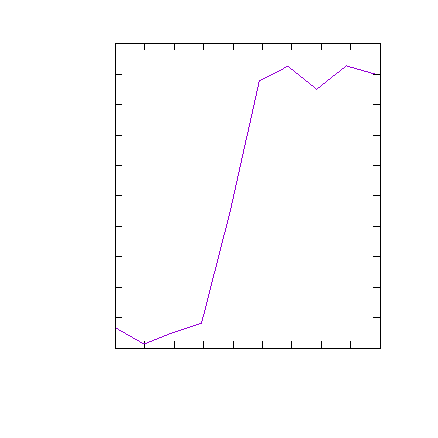
\includegraphics{../images/current}}%
    \gplfronttext
  \end{picture}%
\endgroup

  \caption{Left: Evolution of the ozone concentration after a full stop of the
    generator for different waiting times. Right: ozone level
    dependence on current of Mercury lamp. The steep
    flank occured after a change of the current from
    \SI{10}{\milli\ampere} to \SI{17}{\milli\ampere}.}
  \label{fig:multiple-stop}
\end{figure}

After determining the longtime behaviour, I was interested in
short term pauses. For that reason I stopped the generator (after it
had stabilized) for {\nfrac{} 1/2} \si{hour}, \SI{1}{\hour},
\SI{2}{\hour} and \SI{4}{\hour} and measured the startup time. The
result can be found in Figure~\ref{fig:multiple-stop}
lefthandside. Since the time resolution of the DOAS instrument is
rather coarse the only safe statement is, that even after a
\SI{4}{\hour} stop the concentration climbed back up to around
\SI{200}{ppb} after \SI{5}{\minute}. So it stands to reason, that if
the device is used regularly a prolonged startup time should not be an
issue, even if one sticks to the constant flow of $\Phi_{\ch{O3}} =
\SI{0.03}{\liter\per\minute}$.

As compared to the ozone level in Figure~\ref{fig:long-stop}, the
plateau seems to lie slightly lower in this second experiment. The
reason for this lies most probably in the stabilization of the Mercury
lamp, which was factory new during the first measurements.

After having analyzed the startup procedure, I wanted to investigate
the qualitative influence of the power supply current of the Mercury
lamp on the ozone concentration. Beforehand it was not clear whether a
higher current would increase or decrease the ozone production rate,
as, as was described in Section~\ref{sec:theory-ozone}, I did not know
how a change in power would transform the power distribution on the
different Mercury lines. I recorded a time series while switching
between the two possible currents, \SI{10}{\milli\ampere} and
\SI{17}{\milli\ampere}, and yielded Figure~\ref{fig:multiple-stop}
righthandside. From this one can see that generator still works in a
regime where a higher current leads to more ozone. However, this fact
is secondary in nature for my purposes, as I do not wish to maximize
the ozone output. \SI{200}{ppm} ozone allows for the minimization of
the ozone generator flow entering the sample air stream, minimizing
the effects due to dillution, while still supplying enough ozone for
the conversion. Thus any ozone concentration in this region is well
suited for my purposes, hence I always applied the preset current to
the Mercury lamp.

%%% Local Variables: 
%%% mode: latex
%%% TeX-master: "../Bachelor"
%%% End: 

\subsection{Pure nitrogen monoxide measurements with synthetic air}
\label{sec:no}

After confirming that the generator produced a clean ozone stream, I
turned towards the question, whether it is possible to actually
measure \ch{NO} or not. Furthermore, I wanted to compare the
experimentally necessary reaction tube length to the computed value in
Section~\ref{sec:requirements}.

\subsubsection{Setup}
\label{sec:no-setup}

In order to be able to measure the nitrogen monoxide concentration
directly without additional corrections and computations, I had to
make sure that the used sample air was nitrogen dioxide free. This
lead to the setup depicted in Figure~\ref{fig:no-setup}. I used
synthetic air and \ch{NO} calibration gas with a known \ch{NO}
concentration ($c = \SI{8.177}{ppm}$) together with a mass flow
controller to generate synthetic sample air with a precisely known
\ch{NO} concentration. In order to minimize the influence on the
pressure inside the cavity, I decided to overflow the air inlet
instead of bypassing the cavity pump as is done during a helium
calibration. Thus I set the synthetic air flow to $\Phi_{\text{air}}$
to \SI{3}{\liter\per\minute}. The cavity itself was in the standard
setup described in Section~\ref{sec:inclusion}, except for the
reaction tube length which was varied between \SI{5}{\meter},
\SI{10}{\meter} and \SI{15}{\meter}. For each of these lengths I
varied the \ch{NO} calibration gas flow between \num{0} and
\SI{0.03}{\liter\per\minute}. As zero air I used ambient lab air
together with a zero air cartridge.

\begin{figure}[htbp]
  \centering
  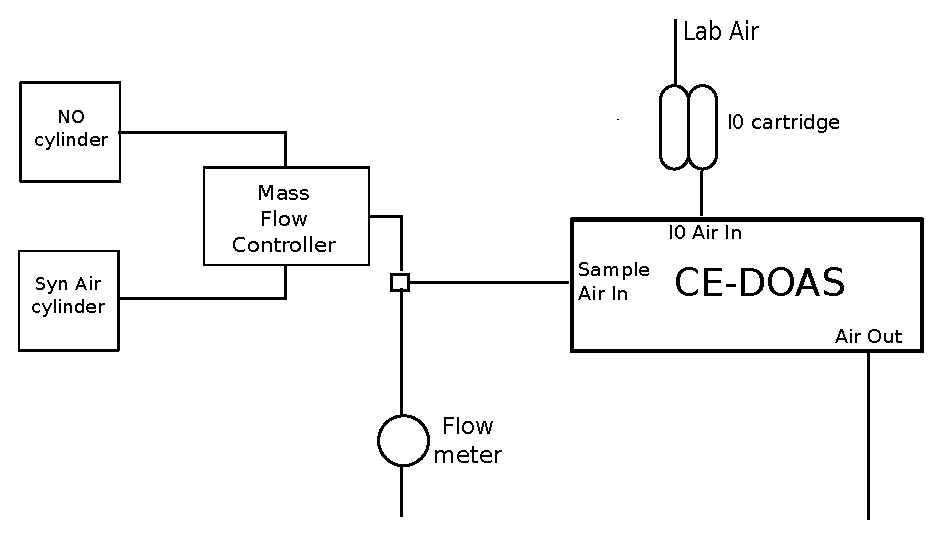
\includegraphics[width=0.6\textwidth]{no_setup.eps}
  \caption{Setup of the calibration measurement.}
  \label{fig:no-setup}
\end{figure}

In order to be able to compare the measured \ch{NO} concentration to the
actual concentration in the air stream, I had to convert the applied
\ch{NO} flow to a concentration, too. I was able to do this using the
following formula
\begin{align}
  c_{\ch{NO}} = c \cdot \frac{\Phi_{\ch{NO}}}{\Phi_{\text{air}} +
  \Phi_{\ch{NO}}}. \label{eq:c-flow}
\end{align}

\subsubsection{Results}
\label{sec:no-results}

Figure~\ref{fig:ts} shows the time series of the \ch{NO} and \ch{O3}
concentration. Each of the three clusters corresponds; from left to
right, to the reaction tube length of \SI{5}{\meter}, \SI{10}{\meter}
and \SI{15}{\meter}. Looking at the ozone concentration on the
left-hand side, it can be seen that its concentration is constant
within its error margins. These, however, are large. This is to be
expected, as the absorption cross section of \ch{O3} in the visual
spectrum is weak compared to the cross section of \ch{NO2} and has
almost no differential structure. Nevertheless, the ozone level seems
acceptably stable, which indicates that not too many ozone destroying
reactions take place, even in the presence of high \ch{NO}
concentrations. This is again what I expected in this very pure sample
air, which should only allow for the oxidation of \ch{NO}. Lastly, the
shape of the ozone time series does not seem to depend on the reaction
tube length.

Looking at the \ch{NO} time series on the right-hand side of
Figure~\ref{fig:ts} the overall shape of the three measurements is
seen to be similar. For the reaction tube length of
$l= \SI{5}{\meter}$ there are slight deviations. The rising flanks
take longer to reach a stable plateau than during the other two
measurements. Furthermore, the first three plateaus are not visible,
however, the reason for this lies in the fact that they were skipped
during the measurement procedure. The behavior of the rising flanks
cannot simply be explained by a too short reaction tube. If this were
the case, the depicted equilibria should all just lay lower, as the
reaction dynamic equilibrium would set for a lower, but
\emph{constant} \ch{NO2} concentration. Interestingly on the falling
flanks the equilibria are reached instantaneously (the small drop at
\SI{50}{ppb} being a human error). One possible explanation might lie
in the adsorption behavior of teflon. For example, if the ozone were
to be adsorbed to the tube walls, this could lead to an effective
increase in ozone concentration, accelerating the reaction and thus
compensating the too short tube length. If, additionally, the
adsorption time scale were in the order of magnitude of the dwell time
per set flow, this could explain why there are slowly increasing
flanks, while the falling flanks stabilize quickly. In the first case
the adsorbed ozone would have to build up because of the increased
concentration, in the second case there would already be enough ozone
adsorbed. Testing this idea was sadly outside the scope of this thesis
which means that for the following measurements I could only accept
this oddity and decided to work with longer tube lengths
(i.\,e.~$l = \SI{10}{\meter}$), which seem to not express this
behavior.


Comparing next the \ch{NO2} plateaus between multiple tube lengths, it
seems that the concentrations seem to coincide. Averaging them and
plotting them against the tube length yields
Figure~\ref{fig:no-length}, which confirms this assertion. The data
points at corresponding flows were linearly interpolated to make
drifts more tangible. The fits were also plotted in the figure. The
interpolation showed that the slope was undiscernible from zero in
each case. At the \SI{5}{\meter} setting one of the red and one of the
violet data points seem to be off. These two data points correspond to
the rising flanks discussed extensively above. It seems that at these
two data points the equilibrium had not been reached and I averaged
too early.

Since Figure~\ref{fig:no-length} indicated that the measured
concentrations are tube length independent (except for the two
outliers), I can use all of them to research the correlation between
the measured concentrations and the ones computed from the flow by
Equation~\eqref{eq:c-flow}. The result can be seen in
Figure~\ref{fig:no-calib} together with a linear regression. The
regression formula yields

\begin{align*}
  y = \num{0.994 \pm 0.002}  \cdot x -\num{0.002 \pm 0.058}.
\end{align*}
Also, I end up with a Pearson's r of 0.994 which further underlines the high
correlation between the measured and the computed data.
\begin{figure}[htbp]
  \centering
  % GNUPLOT: LaTeX picture with Postscript
\begingroup
  \makeatletter
  \providecommand\color[2][]{%
    \GenericError{(gnuplot) \space\space\space\@spaces}{%
      Package color not loaded in conjunction with
      terminal option `colourtext'%
    }{See the gnuplot documentation for explanation.%
    }{Either use 'blacktext' in gnuplot or load the package
      color.sty in LaTeX.}%
    \renewcommand\color[2][]{}%
  }%
  \providecommand\includegraphics[2][]{%
    \GenericError{(gnuplot) \space\space\space\@spaces}{%
      Package graphicx or graphics not loaded%
    }{See the gnuplot documentation for explanation.%
    }{The gnuplot epslatex terminal needs graphicx.sty or graphics.sty.}%
    \renewcommand\includegraphics[2][]{}%
  }%
  \providecommand\rotatebox[2]{#2}%
  \@ifundefined{ifGPcolor}{%
    \newif\ifGPcolor
    \GPcolorfalse
  }{}%
  \@ifundefined{ifGPblacktext}{%
    \newif\ifGPblacktext
    \GPblacktexttrue
  }{}%
  % define a \g@addto@macro without @ in the name:
  \let\gplgaddtomacro\g@addto@macro
  % define empty templates for all commands taking text:
  \gdef\gplbacktext{}%
  \gdef\gplfronttext{}%
  \makeatother
  \ifGPblacktext
    % no textcolor at all
    \def\colorrgb#1{}%
    \def\colorgray#1{}%
  \else
    % gray or color?
    \ifGPcolor
      \def\colorrgb#1{\color[rgb]{#1}}%
      \def\colorgray#1{\color[gray]{#1}}%
      \expandafter\def\csname LTw\endcsname{\color{white}}%
      \expandafter\def\csname LTb\endcsname{\color{black}}%
      \expandafter\def\csname LTa\endcsname{\color{black}}%
      \expandafter\def\csname LT0\endcsname{\color[rgb]{1,0,0}}%
      \expandafter\def\csname LT1\endcsname{\color[rgb]{0,1,0}}%
      \expandafter\def\csname LT2\endcsname{\color[rgb]{0,0,1}}%
      \expandafter\def\csname LT3\endcsname{\color[rgb]{1,0,1}}%
      \expandafter\def\csname LT4\endcsname{\color[rgb]{0,1,1}}%
      \expandafter\def\csname LT5\endcsname{\color[rgb]{1,1,0}}%
      \expandafter\def\csname LT6\endcsname{\color[rgb]{0,0,0}}%
      \expandafter\def\csname LT7\endcsname{\color[rgb]{1,0.3,0}}%
      \expandafter\def\csname LT8\endcsname{\color[rgb]{0.5,0.5,0.5}}%
    \else
      % gray
      \def\colorrgb#1{\color{black}}%
      \def\colorgray#1{\color[gray]{#1}}%
      \expandafter\def\csname LTw\endcsname{\color{white}}%
      \expandafter\def\csname LTb\endcsname{\color{black}}%
      \expandafter\def\csname LTa\endcsname{\color{black}}%
      \expandafter\def\csname LT0\endcsname{\color{black}}%
      \expandafter\def\csname LT1\endcsname{\color{black}}%
      \expandafter\def\csname LT2\endcsname{\color{black}}%
      \expandafter\def\csname LT3\endcsname{\color{black}}%
      \expandafter\def\csname LT4\endcsname{\color{black}}%
      \expandafter\def\csname LT5\endcsname{\color{black}}%
      \expandafter\def\csname LT6\endcsname{\color{black}}%
      \expandafter\def\csname LT7\endcsname{\color{black}}%
      \expandafter\def\csname LT8\endcsname{\color{black}}%
    \fi
  \fi
    \setlength{\unitlength}{0.0500bp}%
    \ifx\gptboxheight\undefined%
      \newlength{\gptboxheight}%
      \newlength{\gptboxwidth}%
      \newsavebox{\gptboxtext}%
    \fi%
    \setlength{\fboxrule}{0.5pt}%
    \setlength{\fboxsep}{1pt}%
\begin{picture}(4030.00,4030.00)%
    \gplgaddtomacro\gplbacktext{%
      \csname LTb\endcsname%
      \put(682,686){\makebox(0,0)[r]{\strut{}$0$}}%
      \put(682,984){\makebox(0,0)[r]{\strut{}$10$}}%
      \put(682,1282){\makebox(0,0)[r]{\strut{}$20$}}%
      \put(682,1580){\makebox(0,0)[r]{\strut{}$30$}}%
      \put(682,1878){\makebox(0,0)[r]{\strut{}$40$}}%
      \put(682,2177){\makebox(0,0)[r]{\strut{}$50$}}%
      \put(682,2475){\makebox(0,0)[r]{\strut{}$60$}}%
      \put(682,2773){\makebox(0,0)[r]{\strut{}$70$}}%
      \put(682,3071){\makebox(0,0)[r]{\strut{}$80$}}%
      \put(682,3369){\makebox(0,0)[r]{\strut{}$90$}}%
      \put(814,554){\rotatebox{-45}{\makebox(0,0)[l]{\strut{}16:00}}}%
      \put(1096,554){\rotatebox{-45}{\makebox(0,0)[l]{\strut{}17:00}}}%
      \put(1378,554){\rotatebox{-45}{\makebox(0,0)[l]{\strut{}18:00}}}%
      \put(1660,554){\rotatebox{-45}{\makebox(0,0)[l]{\strut{}19:00}}}%
      \put(1942,554){\rotatebox{-45}{\makebox(0,0)[l]{\strut{}20:00}}}%
      \put(2224,554){\rotatebox{-45}{\makebox(0,0)[l]{\strut{}21:00}}}%
      \put(2505,554){\rotatebox{-45}{\makebox(0,0)[l]{\strut{}22:00}}}%
      \put(2787,554){\rotatebox{-45}{\makebox(0,0)[l]{\strut{}23:00}}}%
      \put(3069,554){\rotatebox{-45}{\makebox(0,0)[l]{\strut{}00:00}}}%
      \put(3351,554){\rotatebox{-45}{\makebox(0,0)[l]{\strut{}01:00}}}%
      \put(3633,554){\rotatebox{-45}{\makebox(0,0)[l]{\strut{}02:00}}}%
    }%
    \gplgaddtomacro\gplfronttext{%
      \csname LTb\endcsname%
      \put(176,2027){\rotatebox{-270}{\makebox(0,0){\strut{}Concentration [ppb]}}}%
      \put(2223,3699){\makebox(0,0){\strut{}Nitrogen Dioxide}}%
    }%
    \gplbacktext
    \put(0,0){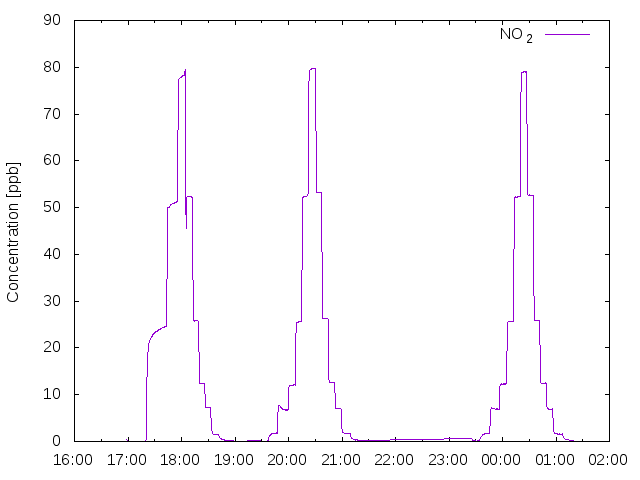
\includegraphics{../images/20160222_NO_fixI0_NO_ts}}%
    \gplfronttext
  \end{picture}%
\endgroup

  \hfill
  % GNUPLOT: LaTeX picture with Postscript
\begingroup
  \makeatletter
  \providecommand\color[2][]{%
    \GenericError{(gnuplot) \space\space\space\@spaces}{%
      Package color not loaded in conjunction with
      terminal option `colourtext'%
    }{See the gnuplot documentation for explanation.%
    }{Either use 'blacktext' in gnuplot or load the package
      color.sty in LaTeX.}%
    \renewcommand\color[2][]{}%
  }%
  \providecommand\includegraphics[2][]{%
    \GenericError{(gnuplot) \space\space\space\@spaces}{%
      Package graphicx or graphics not loaded%
    }{See the gnuplot documentation for explanation.%
    }{The gnuplot epslatex terminal needs graphicx.sty or graphics.sty.}%
    \renewcommand\includegraphics[2][]{}%
  }%
  \providecommand\rotatebox[2]{#2}%
  \@ifundefined{ifGPcolor}{%
    \newif\ifGPcolor
    \GPcolorfalse
  }{}%
  \@ifundefined{ifGPblacktext}{%
    \newif\ifGPblacktext
    \GPblacktexttrue
  }{}%
  % define a \g@addto@macro without @ in the name:
  \let\gplgaddtomacro\g@addto@macro
  % define empty templates for all commands taking text:
  \gdef\gplbacktext{}%
  \gdef\gplfronttext{}%
  \makeatother
  \ifGPblacktext
    % no textcolor at all
    \def\colorrgb#1{}%
    \def\colorgray#1{}%
  \else
    % gray or color?
    \ifGPcolor
      \def\colorrgb#1{\color[rgb]{#1}}%
      \def\colorgray#1{\color[gray]{#1}}%
      \expandafter\def\csname LTw\endcsname{\color{white}}%
      \expandafter\def\csname LTb\endcsname{\color{black}}%
      \expandafter\def\csname LTa\endcsname{\color{black}}%
      \expandafter\def\csname LT0\endcsname{\color[rgb]{1,0,0}}%
      \expandafter\def\csname LT1\endcsname{\color[rgb]{0,1,0}}%
      \expandafter\def\csname LT2\endcsname{\color[rgb]{0,0,1}}%
      \expandafter\def\csname LT3\endcsname{\color[rgb]{1,0,1}}%
      \expandafter\def\csname LT4\endcsname{\color[rgb]{0,1,1}}%
      \expandafter\def\csname LT5\endcsname{\color[rgb]{1,1,0}}%
      \expandafter\def\csname LT6\endcsname{\color[rgb]{0,0,0}}%
      \expandafter\def\csname LT7\endcsname{\color[rgb]{1,0.3,0}}%
      \expandafter\def\csname LT8\endcsname{\color[rgb]{0.5,0.5,0.5}}%
    \else
      % gray
      \def\colorrgb#1{\color{black}}%
      \def\colorgray#1{\color[gray]{#1}}%
      \expandafter\def\csname LTw\endcsname{\color{white}}%
      \expandafter\def\csname LTb\endcsname{\color{black}}%
      \expandafter\def\csname LTa\endcsname{\color{black}}%
      \expandafter\def\csname LT0\endcsname{\color{black}}%
      \expandafter\def\csname LT1\endcsname{\color{black}}%
      \expandafter\def\csname LT2\endcsname{\color{black}}%
      \expandafter\def\csname LT3\endcsname{\color{black}}%
      \expandafter\def\csname LT4\endcsname{\color{black}}%
      \expandafter\def\csname LT5\endcsname{\color{black}}%
      \expandafter\def\csname LT6\endcsname{\color{black}}%
      \expandafter\def\csname LT7\endcsname{\color{black}}%
      \expandafter\def\csname LT8\endcsname{\color{black}}%
    \fi
  \fi
    \setlength{\unitlength}{0.0500bp}%
    \ifx\gptboxheight\undefined%
      \newlength{\gptboxheight}%
      \newlength{\gptboxwidth}%
      \newsavebox{\gptboxtext}%
    \fi%
    \setlength{\fboxrule}{0.5pt}%
    \setlength{\fboxsep}{1pt}%
\begin{picture}(4030.00,4030.00)%
    \gplgaddtomacro\gplbacktext{%
      \csname LTb\endcsname%
      \put(682,686){\makebox(0,0)[r]{\strut{}$-3$}}%
      \put(682,930){\makebox(0,0)[r]{\strut{}$-2$}}%
      \put(682,1174){\makebox(0,0)[r]{\strut{}$-1$}}%
      \put(682,1418){\makebox(0,0)[r]{\strut{}$0$}}%
      \put(682,1662){\makebox(0,0)[r]{\strut{}$1$}}%
      \put(682,1906){\makebox(0,0)[r]{\strut{}$2$}}%
      \put(682,2149){\makebox(0,0)[r]{\strut{}$3$}}%
      \put(682,2393){\makebox(0,0)[r]{\strut{}$4$}}%
      \put(682,2637){\makebox(0,0)[r]{\strut{}$5$}}%
      \put(682,2881){\makebox(0,0)[r]{\strut{}$6$}}%
      \put(682,3125){\makebox(0,0)[r]{\strut{}$7$}}%
      \put(682,3369){\makebox(0,0)[r]{\strut{}$8$}}%
      \put(814,554){\rotatebox{-45}{\makebox(0,0)[l]{\strut{}16:00}}}%
      \put(1096,554){\rotatebox{-45}{\makebox(0,0)[l]{\strut{}17:00}}}%
      \put(1378,554){\rotatebox{-45}{\makebox(0,0)[l]{\strut{}18:00}}}%
      \put(1660,554){\rotatebox{-45}{\makebox(0,0)[l]{\strut{}19:00}}}%
      \put(1942,554){\rotatebox{-45}{\makebox(0,0)[l]{\strut{}20:00}}}%
      \put(2224,554){\rotatebox{-45}{\makebox(0,0)[l]{\strut{}21:00}}}%
      \put(2505,554){\rotatebox{-45}{\makebox(0,0)[l]{\strut{}22:00}}}%
      \put(2787,554){\rotatebox{-45}{\makebox(0,0)[l]{\strut{}23:00}}}%
      \put(3069,554){\rotatebox{-45}{\makebox(0,0)[l]{\strut{}00:00}}}%
      \put(3351,554){\rotatebox{-45}{\makebox(0,0)[l]{\strut{}01:00}}}%
      \put(3633,554){\rotatebox{-45}{\makebox(0,0)[l]{\strut{}02:00}}}%
    }%
    \gplgaddtomacro\gplfronttext{%
      \csname LTb\endcsname%
      \put(176,2027){\rotatebox{-270}{\makebox(0,0){\strut{}Concentration [ppm]}}}%
      \put(2223,3699){\makebox(0,0){\strut{}Ozone}}%
    }%
    \gplbacktext
    \put(0,0){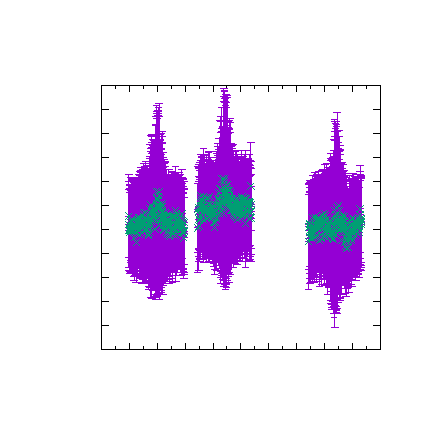
\includegraphics{../images/20160222_NO_fixI0_O3_ts}}%
    \gplfronttext
  \end{picture}%
\endgroup

  \caption{Time series of the \ch{NO2} and \ch{O3} concentration. The
    three clusters correspond to the three used reaction tube lengths
    $l = 5, 10$ and \SI{15}{\meter}.}
  \label{fig:ts}
\end{figure}
\begin{figure}[htbp]
  \centering
  % GNUPLOT: LaTeX picture with Postscript
\begingroup
  \makeatletter
  \providecommand\color[2][]{%
    \GenericError{(gnuplot) \space\space\space\@spaces}{%
      Package color not loaded in conjunction with
      terminal option `colourtext'%
    }{See the gnuplot documentation for explanation.%
    }{Either use 'blacktext' in gnuplot or load the package
      color.sty in LaTeX.}%
    \renewcommand\color[2][]{}%
  }%
  \providecommand\includegraphics[2][]{%
    \GenericError{(gnuplot) \space\space\space\@spaces}{%
      Package graphicx or graphics not loaded%
    }{See the gnuplot documentation for explanation.%
    }{The gnuplot epslatex terminal needs graphicx.sty or graphics.sty.}%
    \renewcommand\includegraphics[2][]{}%
  }%
  \providecommand\rotatebox[2]{#2}%
  \@ifundefined{ifGPcolor}{%
    \newif\ifGPcolor
    \GPcolorfalse
  }{}%
  \@ifundefined{ifGPblacktext}{%
    \newif\ifGPblacktext
    \GPblacktexttrue
  }{}%
  % define a \g@addto@macro without @ in the name:
  \let\gplgaddtomacro\g@addto@macro
  % define empty templates for all commands taking text:
  \gdef\gplbacktext{}%
  \gdef\gplfronttext{}%
  \makeatother
  \ifGPblacktext
    % no textcolor at all
    \def\colorrgb#1{}%
    \def\colorgray#1{}%
  \else
    % gray or color?
    \ifGPcolor
      \def\colorrgb#1{\color[rgb]{#1}}%
      \def\colorgray#1{\color[gray]{#1}}%
      \expandafter\def\csname LTw\endcsname{\color{white}}%
      \expandafter\def\csname LTb\endcsname{\color{black}}%
      \expandafter\def\csname LTa\endcsname{\color{black}}%
      \expandafter\def\csname LT0\endcsname{\color[rgb]{1,0,0}}%
      \expandafter\def\csname LT1\endcsname{\color[rgb]{0,1,0}}%
      \expandafter\def\csname LT2\endcsname{\color[rgb]{0,0,1}}%
      \expandafter\def\csname LT3\endcsname{\color[rgb]{1,0,1}}%
      \expandafter\def\csname LT4\endcsname{\color[rgb]{0,1,1}}%
      \expandafter\def\csname LT5\endcsname{\color[rgb]{1,1,0}}%
      \expandafter\def\csname LT6\endcsname{\color[rgb]{0,0,0}}%
      \expandafter\def\csname LT7\endcsname{\color[rgb]{1,0.3,0}}%
      \expandafter\def\csname LT8\endcsname{\color[rgb]{0.5,0.5,0.5}}%
    \else
      % gray
      \def\colorrgb#1{\color{black}}%
      \def\colorgray#1{\color[gray]{#1}}%
      \expandafter\def\csname LTw\endcsname{\color{white}}%
      \expandafter\def\csname LTb\endcsname{\color{black}}%
      \expandafter\def\csname LTa\endcsname{\color{black}}%
      \expandafter\def\csname LT0\endcsname{\color{black}}%
      \expandafter\def\csname LT1\endcsname{\color{black}}%
      \expandafter\def\csname LT2\endcsname{\color{black}}%
      \expandafter\def\csname LT3\endcsname{\color{black}}%
      \expandafter\def\csname LT4\endcsname{\color{black}}%
      \expandafter\def\csname LT5\endcsname{\color{black}}%
      \expandafter\def\csname LT6\endcsname{\color{black}}%
      \expandafter\def\csname LT7\endcsname{\color{black}}%
      \expandafter\def\csname LT8\endcsname{\color{black}}%
    \fi
  \fi
    \setlength{\unitlength}{0.0500bp}%
    \ifx\gptboxheight\undefined%
      \newlength{\gptboxheight}%
      \newlength{\gptboxwidth}%
      \newsavebox{\gptboxtext}%
    \fi%
    \setlength{\fboxrule}{0.5pt}%
    \setlength{\fboxsep}{1pt}%
\begin{picture}(7200.00,5040.00)%
    \gplgaddtomacro\gplbacktext{%
      \csname LTb\endcsname%
      \put(682,704){\makebox(0,0)[r]{\strut{}$0$}}%
      \put(682,1213){\makebox(0,0)[r]{\strut{}$10$}}%
      \put(682,1722){\makebox(0,0)[r]{\strut{}$20$}}%
      \put(682,2231){\makebox(0,0)[r]{\strut{}$30$}}%
      \put(682,2740){\makebox(0,0)[r]{\strut{}$40$}}%
      \put(682,3248){\makebox(0,0)[r]{\strut{}$50$}}%
      \put(682,3757){\makebox(0,0)[r]{\strut{}$60$}}%
      \put(682,4266){\makebox(0,0)[r]{\strut{}$70$}}%
      \put(682,4775){\makebox(0,0)[r]{\strut{}$80$}}%
      \put(814,484){\makebox(0,0){\strut{}$4$}}%
      \put(1563,484){\makebox(0,0){\strut{}$6$}}%
      \put(2311,484){\makebox(0,0){\strut{}$8$}}%
      \put(3060,484){\makebox(0,0){\strut{}$10$}}%
      \put(3809,484){\makebox(0,0){\strut{}$12$}}%
      \put(4557,484){\makebox(0,0){\strut{}$14$}}%
      \put(5306,484){\makebox(0,0){\strut{}$16$}}%
      \put(6054,484){\makebox(0,0){\strut{}$18$}}%
      \put(6803,484){\makebox(0,0){\strut{}$20$}}%
    }%
    \gplgaddtomacro\gplfronttext{%
      \csname LTb\endcsname%
      \put(176,2739){\rotatebox{-270}{\makebox(0,0){\strut{}Concentration [ppb]}}}%
      \put(3808,154){\makebox(0,0){\strut{}Length [m]}}%
      \csname LTb\endcsname%
      \put(5816,4602){\makebox(0,0)[r]{\strut{}0.01\ \si{\liter\per\minute}}}%
      \csname LTb\endcsname%
      \put(5816,4382){\makebox(0,0)[r]{\strut{}0.03\ \si{\liter\per\minute}}}%
      \csname LTb\endcsname%
      \put(5816,4162){\makebox(0,0)[r]{\strut{}0.05\ \si{\liter\per\minute}}}%
      \csname LTb\endcsname%
      \put(5816,3942){\makebox(0,0)[r]{\strut{}0.1\ \si{\liter\per\minute}}}%
      \csname LTb\endcsname%
      \put(5816,3722){\makebox(0,0)[r]{\strut{}0.2\ \si{\liter\per\minute}}}%
      \csname LTb\endcsname%
      \put(5816,3502){\makebox(0,0)[r]{\strut{}0.3\ \si{\liter\per\minute}}}%
    }%
    \gplbacktext
    \put(0,0){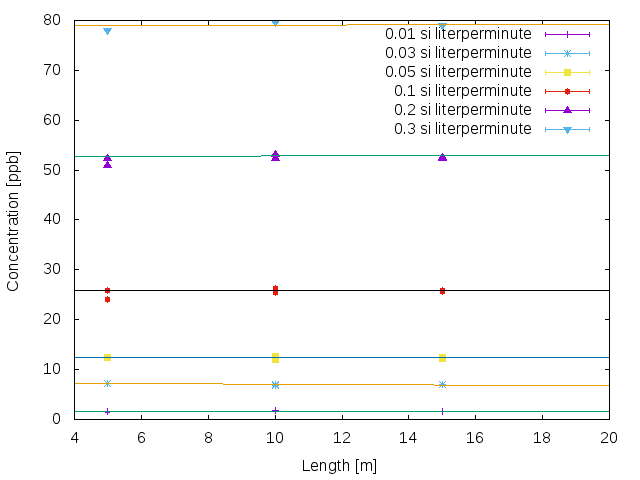
\includegraphics{../images/20160222_NO_fixI0_NO_length}}%
    \gplfronttext
  \end{picture}%
\endgroup

  \caption{\ch{NO} concentration dependence on reaction tube
    length. The data points are colored depending on the applied
    \ch{NO} flow. All data points were linearly interpolated. The
    results can also be found in the plot.}
  \label{fig:no-length}
\end{figure}

\begin{figure}[htbp]
  \centering
  % GNUPLOT: LaTeX picture with Postscript
\begingroup
  \makeatletter
  \providecommand\color[2][]{%
    \GenericError{(gnuplot) \space\space\space\@spaces}{%
      Package color not loaded in conjunction with
      terminal option `colourtext'%
    }{See the gnuplot documentation for explanation.%
    }{Either use 'blacktext' in gnuplot or load the package
      color.sty in LaTeX.}%
    \renewcommand\color[2][]{}%
  }%
  \providecommand\includegraphics[2][]{%
    \GenericError{(gnuplot) \space\space\space\@spaces}{%
      Package graphicx or graphics not loaded%
    }{See the gnuplot documentation for explanation.%
    }{The gnuplot epslatex terminal needs graphicx.sty or graphics.sty.}%
    \renewcommand\includegraphics[2][]{}%
  }%
  \providecommand\rotatebox[2]{#2}%
  \@ifundefined{ifGPcolor}{%
    \newif\ifGPcolor
    \GPcolorfalse
  }{}%
  \@ifundefined{ifGPblacktext}{%
    \newif\ifGPblacktext
    \GPblacktexttrue
  }{}%
  % define a \g@addto@macro without @ in the name:
  \let\gplgaddtomacro\g@addto@macro
  % define empty templates for all commands taking text:
  \gdef\gplbacktext{}%
  \gdef\gplfronttext{}%
  \makeatother
  \ifGPblacktext
    % no textcolor at all
    \def\colorrgb#1{}%
    \def\colorgray#1{}%
  \else
    % gray or color?
    \ifGPcolor
      \def\colorrgb#1{\color[rgb]{#1}}%
      \def\colorgray#1{\color[gray]{#1}}%
      \expandafter\def\csname LTw\endcsname{\color{white}}%
      \expandafter\def\csname LTb\endcsname{\color{black}}%
      \expandafter\def\csname LTa\endcsname{\color{black}}%
      \expandafter\def\csname LT0\endcsname{\color[rgb]{1,0,0}}%
      \expandafter\def\csname LT1\endcsname{\color[rgb]{0,1,0}}%
      \expandafter\def\csname LT2\endcsname{\color[rgb]{0,0,1}}%
      \expandafter\def\csname LT3\endcsname{\color[rgb]{1,0,1}}%
      \expandafter\def\csname LT4\endcsname{\color[rgb]{0,1,1}}%
      \expandafter\def\csname LT5\endcsname{\color[rgb]{1,1,0}}%
      \expandafter\def\csname LT6\endcsname{\color[rgb]{0,0,0}}%
      \expandafter\def\csname LT7\endcsname{\color[rgb]{1,0.3,0}}%
      \expandafter\def\csname LT8\endcsname{\color[rgb]{0.5,0.5,0.5}}%
    \else
      % gray
      \def\colorrgb#1{\color{black}}%
      \def\colorgray#1{\color[gray]{#1}}%
      \expandafter\def\csname LTw\endcsname{\color{white}}%
      \expandafter\def\csname LTb\endcsname{\color{black}}%
      \expandafter\def\csname LTa\endcsname{\color{black}}%
      \expandafter\def\csname LT0\endcsname{\color{black}}%
      \expandafter\def\csname LT1\endcsname{\color{black}}%
      \expandafter\def\csname LT2\endcsname{\color{black}}%
      \expandafter\def\csname LT3\endcsname{\color{black}}%
      \expandafter\def\csname LT4\endcsname{\color{black}}%
      \expandafter\def\csname LT5\endcsname{\color{black}}%
      \expandafter\def\csname LT6\endcsname{\color{black}}%
      \expandafter\def\csname LT7\endcsname{\color{black}}%
      \expandafter\def\csname LT8\endcsname{\color{black}}%
    \fi
  \fi
    \setlength{\unitlength}{0.0500bp}%
    \ifx\gptboxheight\undefined%
      \newlength{\gptboxheight}%
      \newlength{\gptboxwidth}%
      \newsavebox{\gptboxtext}%
    \fi%
    \setlength{\fboxrule}{0.5pt}%
    \setlength{\fboxsep}{1pt}%
\begin{picture}(7776.00,4320.00)%
    \gplgaddtomacro\gplbacktext{%
      \csname LTb\endcsname%
      \put(682,704){\makebox(0,0)[r]{\strut{}$0$}}%
      \put(682,1076){\makebox(0,0)[r]{\strut{}$10$}}%
      \put(682,1449){\makebox(0,0)[r]{\strut{}$20$}}%
      \put(682,1821){\makebox(0,0)[r]{\strut{}$30$}}%
      \put(682,2193){\makebox(0,0)[r]{\strut{}$40$}}%
      \put(682,2566){\makebox(0,0)[r]{\strut{}$50$}}%
      \put(682,2938){\makebox(0,0)[r]{\strut{}$60$}}%
      \put(682,3310){\makebox(0,0)[r]{\strut{}$70$}}%
      \put(682,3683){\makebox(0,0)[r]{\strut{}$80$}}%
      \put(682,4055){\makebox(0,0)[r]{\strut{}$90$}}%
      \put(814,484){\makebox(0,0){\strut{}$0$}}%
      \put(1543,484){\makebox(0,0){\strut{}$10$}}%
      \put(2273,484){\makebox(0,0){\strut{}$20$}}%
      \put(3002,484){\makebox(0,0){\strut{}$30$}}%
      \put(3732,484){\makebox(0,0){\strut{}$40$}}%
      \put(4461,484){\makebox(0,0){\strut{}$50$}}%
      \put(5191,484){\makebox(0,0){\strut{}$60$}}%
      \put(5920,484){\makebox(0,0){\strut{}$70$}}%
      \put(6650,484){\makebox(0,0){\strut{}$80$}}%
      \put(7379,484){\makebox(0,0){\strut{}$90$}}%
    }%
    \gplgaddtomacro\gplfronttext{%
      \csname LTb\endcsname%
      \put(176,2379){\rotatebox{-270}{\makebox(0,0){\strut{}\ch{NO} Concentration, measured with ICAD [ppb]}}}%
      \put(4096,154){\makebox(0,0){\strut{}\ch{NO} Concentration, calculated [ppb]}}%
    }%
    \gplbacktext
    \put(0,0){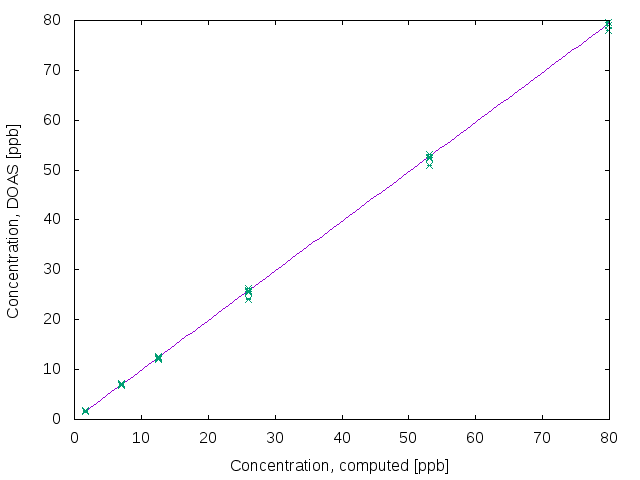
\includegraphics{../images/20160222_NO_fixI0}}%
    \gplfronttext
  \end{picture}%
\endgroup

  \caption{Correlation plot of the computed and the measured \ch{NO}
    concentration.}
  \label{fig:no-calib}
\end{figure}

Thus the deviation between the measured and computed concentration
lies in the per mill regime. Under these controlled conditions the
converter works and does not introduce tangible systematic
errors. Figure~\ref{fig:ts} implies that a \SI{10}{\meter} reaction
tube is appropriate for the setup and will therefore be used for the
following experiments.

%%% Local Variables:
%%% mode: latex
%%% TeX-master: "../Bachelor"
%%% End:

\subsection{Tuning behaviour after ozone switches}
\label{sec:switch}

This measurement was a preliminary measurement to perform the
transition from the pure nitrogen monoxide and synthetic air mixture
to unfiltered ambient air. The new challenge consists in the obvious
fact, that ambient air is not \ch{NO2} free. Thus if one adds ozone to
the sample air stream, one measures \ch{NO_x\, =\ NO + NO2}. In some
cases, e.\,g.\ during live vehicle measurements this is exactly what
is wanted (c.\,f.~Sec.~\ref{sec:vehicle}), however, in other cases it
would be prefered to obtain the nitrogen monoxide and the nitrogen
dioxide concentrations separately. This can only be achieved
indirectly. If there is only a single cavity, one can choose to
measure \ch{NO2} and \ch{NO_x} alternatingly by switching the ozone
stream off and on, I will denote this as \emph{alternating
  measurement mode}. In this case, the technical question arises how
long the time after an ozone switch should be set, such that the
equilibrium is reached and it is safe to perform the next measurement.

As Section~\ref{sec:requirements} indicates, for a tube length of
\SI{15}{\meter} the gas needs about \SI{5.3}{\second} to be
completely exchanged. Taking the cavity volume itself into account a
\SI{30}{\second} purge time should well suffice for the exchange. As
will be seen during this section, there are other unpredicted effects,
which have a far longer decay time. These have to be further
understood before the alternating measurement mode should be used in a
productive system.

\subsubsection{Setup}
\label{sec:switch-setup}

This experiment was performed using the same setup as in
Section~\ref{sec:no} (c.\,f.\ Fig.~\ref{fig:no-setup} on
page~\pageref{fig:no-setup}). I fixed the flow of the \ch{NO}
calibration gas to $\Phi_{\ch{NO}} = \SI{0.01}{\liter\per\minute}$ and
kept all other flows as before. I set the cavity measurement script
to record 60 spectra sampled over 1000 scans each with an exposure
time of \SI{10}{\milli\second} then switch the ozone stream on, record
60 spectra with the same characteristcs, switch the ozone stream off
and repeat. With this setup I got a time resolution of
\SI{10}{\second}. In hindsight the sample size could have been
smaller to improve the time resolution. I performed the measurement
for both \SI{5}{\meter} and \SI{15}{\meter} reaction tube length, due
to time constraints the measurement for \SI{10}{\meter} was shortened
to only collect 30 spectra. Thus I missed some of the decay tail
in this case.

\subsubsection{Results}
\label{sec:switch-results}

Figure~\ref{fig:switch} contains the time series of the measured
\ch{NO2} concentration for a reaction tube length of $l =
\SI{15}{\meter}$. The time series for the other two tube lengths were
similar in shape and are therefore omitted here. The flanks correspond
to the switch in the ozone flow. There are severeal interesting
observations concerning this plot. First of all the increasing flanks
are very steep, which in this setting means, that the transition took
less than \SI{10}{\second}. The decreasing flanks take longer and
interestingly they do not reach \SI{0}{ppb}. This positive offset
could also be observed directly after the start of the measurement
(before any ozone had been added to the 
sample air stream). The concentration rose to a level of
\SI{1.61(2)}{ppb}. One explanation for this is, that the calibration gas is
not \ch{NO2} free. This would raise the question why I did not
measure too much \ch{NO} in Section~\ref{sec:no}, since I actually
measured \ch{NO_x}. This question has three possible answers. First, the
\ch{NO} could have converted to \ch{NO2} over time in a ratio of
one to one. This would explain why I got the right results with the official
container concentration. Alternatively, the official concentration
might not have distinguished between \ch{NO} and \ch{NO2}, but might
have only been talking about a \ch{NO_x} concentration. This second
idea could be rejected after retrieving the calibration method, which
indeed distinguished between \ch{NO} and \ch{NO2}. The last possible
explanation is that the \ch{NO2} concentration might be negligible in
comparison to the amount of \ch{NO}, thus still allowing for the good
result in the previous chapter.

Accepting for the moment that there is a background \ch{NO2} signal, I
turn towards the question, why the decreasing flanks have the slowly
falling tail. In Figure~\ref{fig:switch-pl}, there are falling flanks for
different tube lenghts and one can see that they all appear to have a
similar shape. They all seem to tend to the same equilibrium and the
decay time seems to grow with the tube length. I suspect the reason
for this long tail to be a technical one. Between the ozone valve and
the T-piece, connecting th ozone stream to the sample air stream,
there is a \SI{14}{\centi\meter} tube filled with around
\SI{200}{ppm} ozone. If this diffused into the sample line, this would
lead to further \ch{NO} conversion, although the ozone stream had 
already been switched off. To investigate this hypothesis, I tried to fit
the decay using the following fit formula
\begin{align}
  f(t) \coloneqq c_0 + c_f \cdot\exp\left( -\frac{t}{\tau_f}\right) +
  c_s \cdot \exp\left(-\frac{t}{\tau_s}\right), \label{eq:switch-fit}
\end{align}
i.\,e.\ I suspect two overlaying decay processes. A fast one with a
decay time $\tau_f$ of less than $\SI{10}{\second}$ and a slower one
explaining the tail. Fitting this function I yielded the values
summarized in Table~\ref{tab:switch-coeff}. For the \SI{10}{\meter}
tube length fit the offset concentration had to be fixed to
\SI{1.5}{ppb}, as the measured tail was too short for it to be
determined correctly.

\begin{table}[hbtp]
  \centering
  \begin{tabular}{rSSSSSS}
    \toprule
    {$l$}& {$\tau_f$} & {$\tau_s$} & {$c_0$} & {$c_f$} & {$c_s$} & {$V_{\ch{O3}}$}\\
    {\si{\meter}}& {\si{\second}} & {\si{\second}} & {\si{ppb}} & {\si{ppb}} &
                                                      {\si{ppb}} & {\si{10\tothe{-6}\milli\liter}}\\
    \midrule
    5 & 5.95 \pm 0.13 & 141 \pm 14 & 1.48 \pm 0.03 & 16.5 \pm 0.1 
                      & 1.46 \pm 0.07 & 6.9 \pm 0.8\\
    10 & 7.04 \pm 0.15 & 146 \pm 10 & 1.5 & 19.6 \pm 0.2
                       & 2.1 \pm 0.1 & 10.2 \pm 0.1\\
    15 & 10.15 \pm 0.12 & 193 \pm 12 & 1.52 \pm 0.03 & 21.0 \pm 0.1
                        & 2.36 \pm 0.06 & 15.2 \pm 0.2\\
    \bottomrule
  \end{tabular}
  \caption{Fit coefficients for the decay function
    (Eq.~\eqref{eq:switch-fit}) after an ozone switch off. For the
    pathlength of $l= \SI{10}{\meter}$ the offset concentration was
    fixed to \SI{1.5}{ppb}. This was necessary as, due to the
    shortness of the measurement time, the tail was not long enough
    for the fit to determine the offset correctly. The last column
    contains the (partial) Volume of the ozone participating in the
    reaction to form the long tail.}
  \label{tab:switch-coeff}
\end{table}
In any case the fits underline that  the decay process involves two time
scales. First a rather fast one, which is well described by the time
necessary for the gas to purge the system. And a second time scale in
the order of \SIrange{2.5}{3}{\minute}. To test the dead volume
hypothesis I want to use the fits to determine the amount of ozone
necessary to explain the tail. I assume that the measured \ch{NO2}
signal above the offset, comes directly from the conversion of \ch{NO}
to \ch{NO2}. Looking at Reaction~\eqref{eq:no}, it becomes clear that this
relation leads to a one to one correspondence between the \ch{NO2}
signal\footnote{always above the offset} and the amount of ozone
enetering the sample air stream. To determine the absolute amount, one
has to integrate the slow falling part of the fit function and use the
constant flow of $\Phi = \SI{2}{\liter\per\minute}$ to convert the
result to the (partial) volume of ozone, i.\,e.
\begin{align*}
  V_{\ch{O3}} \coloneqq  c_s \cdot \tau_s \cdot \Phi.
\end{align*}
The result of this computation can be found in
Table~\ref{tab:switch-coeff}, too. A first observation is the clear
pathlength dependence. This is already an indicator against my
hypothesis, as the dead volume is constant. Nevertheless, computing
the ozone volume in the tube leads to
\begin{align*}
  V_{\text{tube}} \approx \SI{3.52e-4}{\milli\liter(ozone)}.
\end{align*}
This is even more evidence that the dead volume cannot be the sole
explanation. The total ozone volume is about two orders of magnitude
too large. Even if I take into account that not the whole tube volume
contributes to the reaction (as the ozone enters the sample air stream
via diffusion), I still have to explain the pathlength
dependence. Especially as it seems that the relation is highly linear,
one might suspect the reason to lie in the adsorption capacity of the
teflon tubes. This capacity would have to be researched more deeply
than I can provide at the current time, however, if the adsorption
plays an important role in the decay behaviour of the system, this
would lead to a further important restriction concerning the
measurement method. The alternating measurment mode would become
impractical to use, as the purge time would have to be in the order of
magnitude of multiple minutes. This is inacceptable for volatile
environments as for example urban areas.

\begin{figure}[htbp]
  \centering
  % GNUPLOT: LaTeX picture with Postscript
\begingroup
  \makeatletter
  \providecommand\color[2][]{%
    \GenericError{(gnuplot) \space\space\space\@spaces}{%
      Package color not loaded in conjunction with
      terminal option `colourtext'%
    }{See the gnuplot documentation for explanation.%
    }{Either use 'blacktext' in gnuplot or load the package
      color.sty in LaTeX.}%
    \renewcommand\color[2][]{}%
  }%
  \providecommand\includegraphics[2][]{%
    \GenericError{(gnuplot) \space\space\space\@spaces}{%
      Package graphicx or graphics not loaded%
    }{See the gnuplot documentation for explanation.%
    }{The gnuplot epslatex terminal needs graphicx.sty or graphics.sty.}%
    \renewcommand\includegraphics[2][]{}%
  }%
  \providecommand\rotatebox[2]{#2}%
  \@ifundefined{ifGPcolor}{%
    \newif\ifGPcolor
    \GPcolorfalse
  }{}%
  \@ifundefined{ifGPblacktext}{%
    \newif\ifGPblacktext
    \GPblacktexttrue
  }{}%
  % define a \g@addto@macro without @ in the name:
  \let\gplgaddtomacro\g@addto@macro
  % define empty templates for all commands taking text:
  \gdef\gplbacktext{}%
  \gdef\gplfronttext{}%
  \makeatother
  \ifGPblacktext
    % no textcolor at all
    \def\colorrgb#1{}%
    \def\colorgray#1{}%
  \else
    % gray or color?
    \ifGPcolor
      \def\colorrgb#1{\color[rgb]{#1}}%
      \def\colorgray#1{\color[gray]{#1}}%
      \expandafter\def\csname LTw\endcsname{\color{white}}%
      \expandafter\def\csname LTb\endcsname{\color{black}}%
      \expandafter\def\csname LTa\endcsname{\color{black}}%
      \expandafter\def\csname LT0\endcsname{\color[rgb]{1,0,0}}%
      \expandafter\def\csname LT1\endcsname{\color[rgb]{0,1,0}}%
      \expandafter\def\csname LT2\endcsname{\color[rgb]{0,0,1}}%
      \expandafter\def\csname LT3\endcsname{\color[rgb]{1,0,1}}%
      \expandafter\def\csname LT4\endcsname{\color[rgb]{0,1,1}}%
      \expandafter\def\csname LT5\endcsname{\color[rgb]{1,1,0}}%
      \expandafter\def\csname LT6\endcsname{\color[rgb]{0,0,0}}%
      \expandafter\def\csname LT7\endcsname{\color[rgb]{1,0.3,0}}%
      \expandafter\def\csname LT8\endcsname{\color[rgb]{0.5,0.5,0.5}}%
    \else
      % gray
      \def\colorrgb#1{\color{black}}%
      \def\colorgray#1{\color[gray]{#1}}%
      \expandafter\def\csname LTw\endcsname{\color{white}}%
      \expandafter\def\csname LTb\endcsname{\color{black}}%
      \expandafter\def\csname LTa\endcsname{\color{black}}%
      \expandafter\def\csname LT0\endcsname{\color{black}}%
      \expandafter\def\csname LT1\endcsname{\color{black}}%
      \expandafter\def\csname LT2\endcsname{\color{black}}%
      \expandafter\def\csname LT3\endcsname{\color{black}}%
      \expandafter\def\csname LT4\endcsname{\color{black}}%
      \expandafter\def\csname LT5\endcsname{\color{black}}%
      \expandafter\def\csname LT6\endcsname{\color{black}}%
      \expandafter\def\csname LT7\endcsname{\color{black}}%
      \expandafter\def\csname LT8\endcsname{\color{black}}%
    \fi
  \fi
    \setlength{\unitlength}{0.0500bp}%
    \ifx\gptboxheight\undefined%
      \newlength{\gptboxheight}%
      \newlength{\gptboxwidth}%
      \newsavebox{\gptboxtext}%
    \fi%
    \setlength{\fboxrule}{0.5pt}%
    \setlength{\fboxsep}{1pt}%
\begin{picture}(7200.00,5040.00)%
    \gplgaddtomacro\gplbacktext{%
      \csname LTb\endcsname%
      \put(682,704){\makebox(0,0)[r]{\strut{}$0$}}%
      \put(682,1383){\makebox(0,0)[r]{\strut{}$5$}}%
      \put(682,2061){\makebox(0,0)[r]{\strut{}$10$}}%
      \put(682,2740){\makebox(0,0)[r]{\strut{}$15$}}%
      \put(682,3418){\makebox(0,0)[r]{\strut{}$20$}}%
      \put(682,4097){\makebox(0,0)[r]{\strut{}$25$}}%
      \put(682,4775){\makebox(0,0)[r]{\strut{}$30$}}%
      \put(814,484){\makebox(0,0){\strut{}$0$}}%
      \put(1563,484){\makebox(0,0){\strut{}$500$}}%
      \put(2311,484){\makebox(0,0){\strut{}$1000$}}%
      \put(3060,484){\makebox(0,0){\strut{}$1500$}}%
      \put(3809,484){\makebox(0,0){\strut{}$2000$}}%
      \put(4557,484){\makebox(0,0){\strut{}$2500$}}%
      \put(5306,484){\makebox(0,0){\strut{}$3000$}}%
      \put(6054,484){\makebox(0,0){\strut{}$3500$}}%
      \put(6803,484){\makebox(0,0){\strut{}$4000$}}%
    }%
    \gplgaddtomacro\gplfronttext{%
      \csname LTb\endcsname%
      \put(176,2739){\rotatebox{-270}{\makebox(0,0){\strut{}Concentration [ppb]}}}%
      \put(3808,154){\makebox(0,0){\strut{}Time [s]}}%
    }%
    \gplbacktext
    \put(0,0){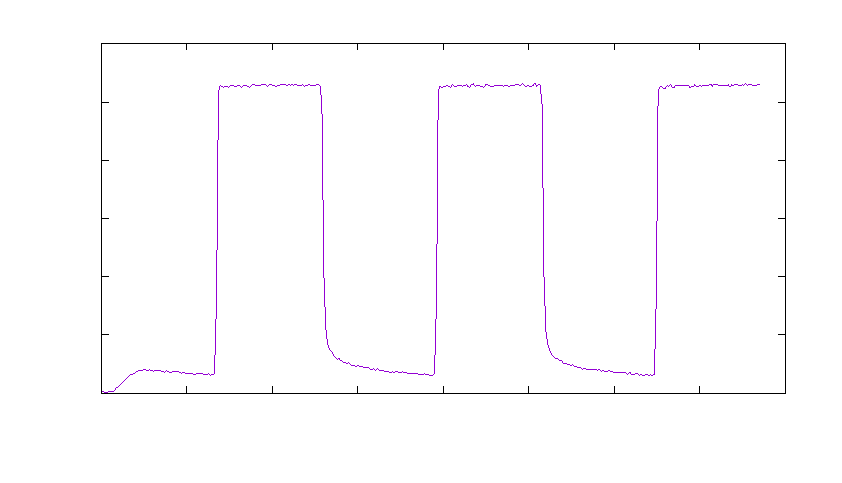
\includegraphics{../images/20160223_15_equil_fixI0_ts}}%
    \gplfronttext
  \end{picture}%
\endgroup

  \caption{Timeseries of the measured \ch{NO2} concentration while
    switching the ozone stream on and off.}
  \label{fig:switch}
\end{figure}
\begin{figure}[htbp]
  \centering
  % GNUPLOT: LaTeX picture with Postscript
\begingroup
  \makeatletter
  \providecommand\color[2][]{%
    \GenericError{(gnuplot) \space\space\space\@spaces}{%
      Package color not loaded in conjunction with
      terminal option `colourtext'%
    }{See the gnuplot documentation for explanation.%
    }{Either use 'blacktext' in gnuplot or load the package
      color.sty in LaTeX.}%
    \renewcommand\color[2][]{}%
  }%
  \providecommand\includegraphics[2][]{%
    \GenericError{(gnuplot) \space\space\space\@spaces}{%
      Package graphicx or graphics not loaded%
    }{See the gnuplot documentation for explanation.%
    }{The gnuplot epslatex terminal needs graphicx.sty or graphics.sty.}%
    \renewcommand\includegraphics[2][]{}%
  }%
  \providecommand\rotatebox[2]{#2}%
  \@ifundefined{ifGPcolor}{%
    \newif\ifGPcolor
    \GPcolorfalse
  }{}%
  \@ifundefined{ifGPblacktext}{%
    \newif\ifGPblacktext
    \GPblacktexttrue
  }{}%
  % define a \g@addto@macro without @ in the name:
  \let\gplgaddtomacro\g@addto@macro
  % define empty templates for all commands taking text:
  \gdef\gplbacktext{}%
  \gdef\gplfronttext{}%
  \makeatother
  \ifGPblacktext
    % no textcolor at all
    \def\colorrgb#1{}%
    \def\colorgray#1{}%
  \else
    % gray or color?
    \ifGPcolor
      \def\colorrgb#1{\color[rgb]{#1}}%
      \def\colorgray#1{\color[gray]{#1}}%
      \expandafter\def\csname LTw\endcsname{\color{white}}%
      \expandafter\def\csname LTb\endcsname{\color{black}}%
      \expandafter\def\csname LTa\endcsname{\color{black}}%
      \expandafter\def\csname LT0\endcsname{\color[rgb]{1,0,0}}%
      \expandafter\def\csname LT1\endcsname{\color[rgb]{0,1,0}}%
      \expandafter\def\csname LT2\endcsname{\color[rgb]{0,0,1}}%
      \expandafter\def\csname LT3\endcsname{\color[rgb]{1,0,1}}%
      \expandafter\def\csname LT4\endcsname{\color[rgb]{0,1,1}}%
      \expandafter\def\csname LT5\endcsname{\color[rgb]{1,1,0}}%
      \expandafter\def\csname LT6\endcsname{\color[rgb]{0,0,0}}%
      \expandafter\def\csname LT7\endcsname{\color[rgb]{1,0.3,0}}%
      \expandafter\def\csname LT8\endcsname{\color[rgb]{0.5,0.5,0.5}}%
    \else
      % gray
      \def\colorrgb#1{\color{black}}%
      \def\colorgray#1{\color[gray]{#1}}%
      \expandafter\def\csname LTw\endcsname{\color{white}}%
      \expandafter\def\csname LTb\endcsname{\color{black}}%
      \expandafter\def\csname LTa\endcsname{\color{black}}%
      \expandafter\def\csname LT0\endcsname{\color{black}}%
      \expandafter\def\csname LT1\endcsname{\color{black}}%
      \expandafter\def\csname LT2\endcsname{\color{black}}%
      \expandafter\def\csname LT3\endcsname{\color{black}}%
      \expandafter\def\csname LT4\endcsname{\color{black}}%
      \expandafter\def\csname LT5\endcsname{\color{black}}%
      \expandafter\def\csname LT6\endcsname{\color{black}}%
      \expandafter\def\csname LT7\endcsname{\color{black}}%
      \expandafter\def\csname LT8\endcsname{\color{black}}%
    \fi
  \fi
    \setlength{\unitlength}{0.0500bp}%
    \ifx\gptboxheight\undefined%
      \newlength{\gptboxheight}%
      \newlength{\gptboxwidth}%
      \newsavebox{\gptboxtext}%
    \fi%
    \setlength{\fboxrule}{0.5pt}%
    \setlength{\fboxsep}{1pt}%
\begin{picture}(7200.00,5040.00)%
    \gplgaddtomacro\gplbacktext{%
      \csname LTb\endcsname%
      \put(682,704){\makebox(0,0)[r]{\strut{}$0$}}%
      \put(682,1518){\makebox(0,0)[r]{\strut{}$5$}}%
      \put(682,2332){\makebox(0,0)[r]{\strut{}$10$}}%
      \put(682,3147){\makebox(0,0)[r]{\strut{}$15$}}%
      \put(682,3961){\makebox(0,0)[r]{\strut{}$20$}}%
      \put(682,4775){\makebox(0,0)[r]{\strut{}$25$}}%
      \put(814,484){\makebox(0,0){\strut{}$0$}}%
      \put(1670,484){\makebox(0,0){\strut{}$100$}}%
      \put(2525,484){\makebox(0,0){\strut{}$200$}}%
      \put(3381,484){\makebox(0,0){\strut{}$300$}}%
      \put(4236,484){\makebox(0,0){\strut{}$400$}}%
      \put(5092,484){\makebox(0,0){\strut{}$500$}}%
      \put(5947,484){\makebox(0,0){\strut{}$600$}}%
      \put(6803,484){\makebox(0,0){\strut{}$700$}}%
    }%
    \gplgaddtomacro\gplfronttext{%
      \csname LTb\endcsname%
      \put(176,2739){\rotatebox{-270}{\makebox(0,0){\strut{}Concentration [ppb]}}}%
      \put(3808,154){\makebox(0,0){\strut{}Time [s]}}%
      \csname LTb\endcsname%
      \put(5816,4602){\makebox(0,0)[r]{\strut{}$\SI{05}{\meter}$}}%
      \csname LTb\endcsname%
      \put(5816,4382){\makebox(0,0)[r]{\strut{}$\SI{10}{\meter}$}}%
      \csname LTb\endcsname%
      \put(5816,4162){\makebox(0,0)[r]{\strut{}$\SI{15}{\meter}$}}%
    }%
    \gplbacktext
    \put(0,0){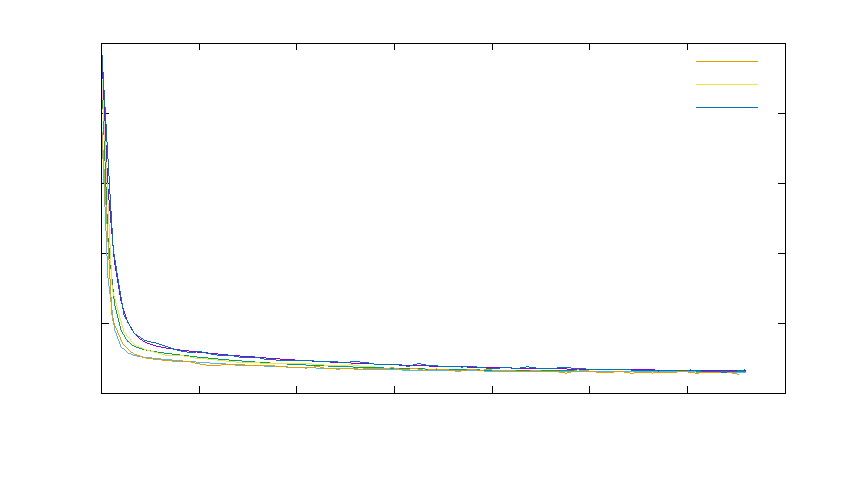
\includegraphics{../images/20160223_equil_fixI0_fall_fit}}%
    \gplfronttext
  \end{picture}%
\endgroup

  \caption{The behaviour of the falling flanks depending on the
    reaction pathlength}
  \label{fig:switch-pl}
\end{figure}

If the alternating mode is to be used anyways, one would have to
compensate for the long tail. For the laboratory conditions, used in
this experiment, supply of \ch{NO} was constant,
such that the behaviour of the falling flank is solely determined by
the changing ozone concentration. Assuming that the decay always
follows Equation~\eqref{eq:switch-fit} with the coefficients given in
Table~\ref{tab:switch-coeff}, the average additional
\ch{NO2} signal due to the flank can be computed by

\begin{align}
  \bar c_s = \frac{c_s}{\Delta t} \int_{t_0}^{t_1}
  \exp\left(-\frac{t}{\tau_s}\right)\d[t] \approx \SI{1.55(8)}{ppb},\label{eq:offset}
\end{align}
with $t_0 = \SI{30}{\second}$, $t_1 = \SI{60}{\second}$,
$\Delta t = t_1 - t_0$, where I already specialised to the later used
setup of $l = \SI{10}{\meter}$. I propose now to correct the measured
\ch{NO2} values by this offset. For this procedure to work, the decay
form would need to be mainly \ch{NO} independent. This assumption
might be true, as the bottle neck in Reaction~\eqref{eq:no} should be
the vanishing ozone. However, to be sure, I would suggest to perform
further decay experiments at multiple \ch{NO} levels. This would lead
to the further advantage, that possible existing \ch{NO} dependencies
could possibly be extrapolated. This then could lead to a \ch{NO_x}
dependent offset correction in the evaluation procedure.  In the
following I tested the limits of this rather crude approximation. The
results can be found in the next section.

%%% Local Variables:
%%% mode: latex
%%% TeX-master: "../Bachelor"
%%% End:

\subsection{Comparison to chemiluminescence measurements}
\label{sec:cld}

After having assured the functionality of the converter in the lab
environment, I wanted to use it with ambient air. I wanted to try out
the alternating measurement mode described in the previous section and
compare the results to another nitrogen monoxide measurement
instrument, a chemiluminescence monitor (or display, short: cld). This
made it possible to work in a more realistic setting while
simultaneously being able to verify the converter results.

\subsubsection{Setup}
\label{sec:cld-setup}

The \ch{NO_x} ICAD and the chemiluminescence monitor (Eco Physics CLD
770 AL ppt Chemiluminescence \ch{NO} Analyzer) were both setup at the
rooftop laboratory at the Institute of Environmental Physics. I used
a tripod on the roof together with two teflon tubes to make sure to
sample at the same spot with both instruments.

I set up the ICAD measurement cell as described in
Section~\ref{sec:inclusion}. For each spectrum I sampled 3000 spectra
at an exposure time of \SI{10}{\milli\second}. Furthermore, I used a
purge time of \SI{30}{\second} after ozone switches. This time was set
too short to account for the slowly falling tail, as
Section~\ref{sec:switch} indicates.

In order to account for slight differences in the path length and
flows in the two instruments, I decided to compute \SI{30}{\minute}
averages for the comparison. These measurements were taken during the
day of January 22 and January 25, 2016.

\subsubsection{Results}
\label{sec:cld-results}

The time series of the two measurements can be found in
Figure~\ref{fig:corr-ts}. As can be seen, the qualitative form of the
\ch{NO_x} ICAD results is in good accordance with the
chemiluminescence results.  However, there seems to be an offset and
the concentration, measured by the \ch{NO_x} ICAD, is systematically
lower than the chemiluminescence concentration. This relation is also
plainly visible in the correlation plot in
Figure~\ref{fig:cld-corr}. The measurements are very well correlated
and can be easily fitted by a linear regression, but the line has an
offset and a slope, which is differing from unity:

\begin{align*}
  y = \SI{1.38}{{ppb}\tothe{-1}} \cdot x + 3.8.
\end{align*}

There were two avenues I followed in an attempt to understand these
findings. Both of them follow arguments already layed out in
Section~\ref{sec:switch}. The first consists in the observation that
the \ch{NO} calibration gas container was used to calibrate the
chemiluminescence display. If some of the \ch{NO} had been converted
to \ch{NO2}, there would be an error in the chemiluminescence
calibration, which would lead to an overestimation of the \ch{NO}
concentration by the cld. Using the \ch{NO2} offset found in the
previous section, it is possible compute that there is about
\SI{420}{ppb} \ch{NO2} in the cylinder, if all of it stemmed from
\ch{NO} this would introduce an error of about \SI{5}{\percent} (the
calibration concentration given was $c = \SI{8.177}{ppm}$). This is
not enough to explain the discrepancy. Together with the fact that I
still cannot explain, how the transition from \ch{NO} to \ch{NO2}
could occur, I discarded this approach.

The second avenue I took was to look at the purge time.
Section~\ref{sec:switch} suggests that \SI{30}{\second} purge time is
not enough after the ozone switch has been turned off. Thus one would
expect the measured \ch{NO2} intensities to be overestimated. One
observation pointing towards the influence of this effect is, that I
measured negative \ch{NO} concentrations (to a minimum of
\SI{-1.54}{ppb}), which is of course absurd. In the previous section I
suggested that the surplus \ch{NO2} signal does not depend too strongly
on the \ch{NO} concentration. If this assumption is correct, one will
expect to be able to mitigate the effects by lowering the \ch{NO2}
signal by $\bar c_s = \SI{1.55}{ppb}$ (c.\,f.\
Equation~\eqref{eq:offset} on page~\pageref{eq:offset}), which
corresponds surprisingly well to the negative offset of the measured
data. This \emph{tail corrected} data set was then again correlated
with the chemiluminescence data. The result can also be found in
Figure~\ref{fig:cld-corr}. The linear regression follows the formula
\begin{align*}
  y = \SI{1.38}{ppb\tothe{-1}} \cdot x + 1.67.
\end{align*}
So the tail correction has only an effect on the intercept of the
regression. This is expected as the constant lowering of the \ch{NO2}
signal increases the computed \ch{NO} signal by the same amount and
thus all data points are shifted to the right. Hence the slope of the
regression is still off. Clearly, the approach utilized here was too
simplistic to account for all effects. Further investigations are
necessary to understand the required corrections. Possibly, the
\ch{NO2} correction can be computed utilizing the previous \ch{NO_x}
data point, thus indirectly taking \ch{NO} influences on the offset
into account. This varying \ch{NO2} correction could then also
influence the slope of the regression. In order to investigate this
further, I suggest to perform additional decay measurements as
proposed in the previous section.

\begin{figure}[htbp]
  \centering
  % GNUPLOT: LaTeX picture with Postscript
\begingroup
  \makeatletter
  \providecommand\color[2][]{%
    \GenericError{(gnuplot) \space\space\space\@spaces}{%
      Package color not loaded in conjunction with
      terminal option `colourtext'%
    }{See the gnuplot documentation for explanation.%
    }{Either use 'blacktext' in gnuplot or load the package
      color.sty in LaTeX.}%
    \renewcommand\color[2][]{}%
  }%
  \providecommand\includegraphics[2][]{%
    \GenericError{(gnuplot) \space\space\space\@spaces}{%
      Package graphicx or graphics not loaded%
    }{See the gnuplot documentation for explanation.%
    }{The gnuplot epslatex terminal needs graphicx.sty or graphics.sty.}%
    \renewcommand\includegraphics[2][]{}%
  }%
  \providecommand\rotatebox[2]{#2}%
  \@ifundefined{ifGPcolor}{%
    \newif\ifGPcolor
    \GPcolorfalse
  }{}%
  \@ifundefined{ifGPblacktext}{%
    \newif\ifGPblacktext
    \GPblacktexttrue
  }{}%
  % define a \g@addto@macro without @ in the name:
  \let\gplgaddtomacro\g@addto@macro
  % define empty templates for all commands taking text:
  \gdef\gplbacktext{}%
  \gdef\gplfronttext{}%
  \makeatother
  \ifGPblacktext
    % no textcolor at all
    \def\colorrgb#1{}%
    \def\colorgray#1{}%
  \else
    % gray or color?
    \ifGPcolor
      \def\colorrgb#1{\color[rgb]{#1}}%
      \def\colorgray#1{\color[gray]{#1}}%
      \expandafter\def\csname LTw\endcsname{\color{white}}%
      \expandafter\def\csname LTb\endcsname{\color{black}}%
      \expandafter\def\csname LTa\endcsname{\color{black}}%
      \expandafter\def\csname LT0\endcsname{\color[rgb]{1,0,0}}%
      \expandafter\def\csname LT1\endcsname{\color[rgb]{0,1,0}}%
      \expandafter\def\csname LT2\endcsname{\color[rgb]{0,0,1}}%
      \expandafter\def\csname LT3\endcsname{\color[rgb]{1,0,1}}%
      \expandafter\def\csname LT4\endcsname{\color[rgb]{0,1,1}}%
      \expandafter\def\csname LT5\endcsname{\color[rgb]{1,1,0}}%
      \expandafter\def\csname LT6\endcsname{\color[rgb]{0,0,0}}%
      \expandafter\def\csname LT7\endcsname{\color[rgb]{1,0.3,0}}%
      \expandafter\def\csname LT8\endcsname{\color[rgb]{0.5,0.5,0.5}}%
    \else
      % gray
      \def\colorrgb#1{\color{black}}%
      \def\colorgray#1{\color[gray]{#1}}%
      \expandafter\def\csname LTw\endcsname{\color{white}}%
      \expandafter\def\csname LTb\endcsname{\color{black}}%
      \expandafter\def\csname LTa\endcsname{\color{black}}%
      \expandafter\def\csname LT0\endcsname{\color{black}}%
      \expandafter\def\csname LT1\endcsname{\color{black}}%
      \expandafter\def\csname LT2\endcsname{\color{black}}%
      \expandafter\def\csname LT3\endcsname{\color{black}}%
      \expandafter\def\csname LT4\endcsname{\color{black}}%
      \expandafter\def\csname LT5\endcsname{\color{black}}%
      \expandafter\def\csname LT6\endcsname{\color{black}}%
      \expandafter\def\csname LT7\endcsname{\color{black}}%
      \expandafter\def\csname LT8\endcsname{\color{black}}%
    \fi
  \fi
    \setlength{\unitlength}{0.0500bp}%
    \ifx\gptboxheight\undefined%
      \newlength{\gptboxheight}%
      \newlength{\gptboxwidth}%
      \newsavebox{\gptboxtext}%
    \fi%
    \setlength{\fboxrule}{0.5pt}%
    \setlength{\fboxsep}{1pt}%
\begin{picture}(3888.00,3888.00)%
    \gplgaddtomacro\gplbacktext{%
      \csname LTb\endcsname%
      \put(682,686){\makebox(0,0)[r]{\strut{}$-5$}}%
      \put(682,917){\makebox(0,0)[r]{\strut{}$0$}}%
      \put(682,1148){\makebox(0,0)[r]{\strut{}$5$}}%
      \put(682,1379){\makebox(0,0)[r]{\strut{}$10$}}%
      \put(682,1610){\makebox(0,0)[r]{\strut{}$15$}}%
      \put(682,1841){\makebox(0,0)[r]{\strut{}$20$}}%
      \put(682,2072){\makebox(0,0)[r]{\strut{}$25$}}%
      \put(682,2303){\makebox(0,0)[r]{\strut{}$30$}}%
      \put(682,2534){\makebox(0,0)[r]{\strut{}$35$}}%
      \put(682,2765){\makebox(0,0)[r]{\strut{}$40$}}%
      \put(682,2996){\makebox(0,0)[r]{\strut{}$45$}}%
      \put(682,3227){\makebox(0,0)[r]{\strut{}$50$}}%
      \put(814,554){\rotatebox{-45}{\makebox(0,0)[l]{\strut{}16:00}}}%
      \put(1149,554){\rotatebox{-45}{\makebox(0,0)[l]{\strut{}17:00}}}%
      \put(1483,554){\rotatebox{-45}{\makebox(0,0)[l]{\strut{}18:00}}}%
      \put(1818,554){\rotatebox{-45}{\makebox(0,0)[l]{\strut{}19:00}}}%
      \put(2153,554){\rotatebox{-45}{\makebox(0,0)[l]{\strut{}20:00}}}%
      \put(2487,554){\rotatebox{-45}{\makebox(0,0)[l]{\strut{}21:00}}}%
      \put(2822,554){\rotatebox{-45}{\makebox(0,0)[l]{\strut{}22:00}}}%
      \put(3156,554){\rotatebox{-45}{\makebox(0,0)[l]{\strut{}23:00}}}%
      \put(3491,554){\rotatebox{-45}{\makebox(0,0)[l]{\strut{}00:00}}}%
    }%
    \gplgaddtomacro\gplfronttext{%
      \csname LTb\endcsname%
      \put(176,1956){\rotatebox{-270}{\makebox(0,0){\strut{}\ch{NO} Concentration [ppb]}}}%
      \put(2152,3557){\makebox(0,0){\strut{}January 22, 2016}}%
    }%
    \gplbacktext
    \put(0,0){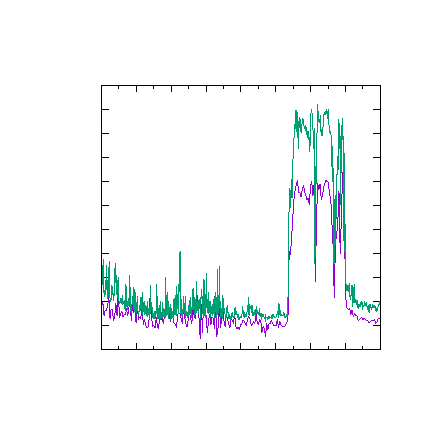
\includegraphics{../images/correlation_ts01}}%
    \gplfronttext
  \end{picture}%
\endgroup

  \hfill
  % GNUPLOT: LaTeX picture with Postscript
\begingroup
  \makeatletter
  \providecommand\color[2][]{%
    \GenericError{(gnuplot) \space\space\space\@spaces}{%
      Package color not loaded in conjunction with
      terminal option `colourtext'%
    }{See the gnuplot documentation for explanation.%
    }{Either use 'blacktext' in gnuplot or load the package
      color.sty in LaTeX.}%
    \renewcommand\color[2][]{}%
  }%
  \providecommand\includegraphics[2][]{%
    \GenericError{(gnuplot) \space\space\space\@spaces}{%
      Package graphicx or graphics not loaded%
    }{See the gnuplot documentation for explanation.%
    }{The gnuplot epslatex terminal needs graphicx.sty or graphics.sty.}%
    \renewcommand\includegraphics[2][]{}%
  }%
  \providecommand\rotatebox[2]{#2}%
  \@ifundefined{ifGPcolor}{%
    \newif\ifGPcolor
    \GPcolorfalse
  }{}%
  \@ifundefined{ifGPblacktext}{%
    \newif\ifGPblacktext
    \GPblacktexttrue
  }{}%
  % define a \g@addto@macro without @ in the name:
  \let\gplgaddtomacro\g@addto@macro
  % define empty templates for all commands taking text:
  \gdef\gplbacktext{}%
  \gdef\gplfronttext{}%
  \makeatother
  \ifGPblacktext
    % no textcolor at all
    \def\colorrgb#1{}%
    \def\colorgray#1{}%
  \else
    % gray or color?
    \ifGPcolor
      \def\colorrgb#1{\color[rgb]{#1}}%
      \def\colorgray#1{\color[gray]{#1}}%
      \expandafter\def\csname LTw\endcsname{\color{white}}%
      \expandafter\def\csname LTb\endcsname{\color{black}}%
      \expandafter\def\csname LTa\endcsname{\color{black}}%
      \expandafter\def\csname LT0\endcsname{\color[rgb]{1,0,0}}%
      \expandafter\def\csname LT1\endcsname{\color[rgb]{0,1,0}}%
      \expandafter\def\csname LT2\endcsname{\color[rgb]{0,0,1}}%
      \expandafter\def\csname LT3\endcsname{\color[rgb]{1,0,1}}%
      \expandafter\def\csname LT4\endcsname{\color[rgb]{0,1,1}}%
      \expandafter\def\csname LT5\endcsname{\color[rgb]{1,1,0}}%
      \expandafter\def\csname LT6\endcsname{\color[rgb]{0,0,0}}%
      \expandafter\def\csname LT7\endcsname{\color[rgb]{1,0.3,0}}%
      \expandafter\def\csname LT8\endcsname{\color[rgb]{0.5,0.5,0.5}}%
    \else
      % gray
      \def\colorrgb#1{\color{black}}%
      \def\colorgray#1{\color[gray]{#1}}%
      \expandafter\def\csname LTw\endcsname{\color{white}}%
      \expandafter\def\csname LTb\endcsname{\color{black}}%
      \expandafter\def\csname LTa\endcsname{\color{black}}%
      \expandafter\def\csname LT0\endcsname{\color{black}}%
      \expandafter\def\csname LT1\endcsname{\color{black}}%
      \expandafter\def\csname LT2\endcsname{\color{black}}%
      \expandafter\def\csname LT3\endcsname{\color{black}}%
      \expandafter\def\csname LT4\endcsname{\color{black}}%
      \expandafter\def\csname LT5\endcsname{\color{black}}%
      \expandafter\def\csname LT6\endcsname{\color{black}}%
      \expandafter\def\csname LT7\endcsname{\color{black}}%
      \expandafter\def\csname LT8\endcsname{\color{black}}%
    \fi
  \fi
    \setlength{\unitlength}{0.0500bp}%
    \ifx\gptboxheight\undefined%
      \newlength{\gptboxheight}%
      \newlength{\gptboxwidth}%
      \newsavebox{\gptboxtext}%
    \fi%
    \setlength{\fboxrule}{0.5pt}%
    \setlength{\fboxsep}{1pt}%
\begin{picture}(3888.00,3888.00)%
    \gplgaddtomacro\gplbacktext{%
      \csname LTb\endcsname%
      \put(814,686){\makebox(0,0)[r]{\strut{}$-10$}}%
      \put(814,1049){\makebox(0,0)[r]{\strut{}$0$}}%
      \put(814,1412){\makebox(0,0)[r]{\strut{}$10$}}%
      \put(814,1775){\makebox(0,0)[r]{\strut{}$20$}}%
      \put(814,2138){\makebox(0,0)[r]{\strut{}$30$}}%
      \put(814,2501){\makebox(0,0)[r]{\strut{}$40$}}%
      \put(814,2864){\makebox(0,0)[r]{\strut{}$50$}}%
      \put(814,3227){\makebox(0,0)[r]{\strut{}$60$}}%
      \put(946,554){\rotatebox{-45}{\makebox(0,0)[l]{\strut{}08:00}}}%
      \put(1264,554){\rotatebox{-45}{\makebox(0,0)[l]{\strut{}10:00}}}%
      \put(1582,554){\rotatebox{-45}{\makebox(0,0)[l]{\strut{}12:00}}}%
      \put(1900,554){\rotatebox{-45}{\makebox(0,0)[l]{\strut{}14:00}}}%
      \put(2219,554){\rotatebox{-45}{\makebox(0,0)[l]{\strut{}16:00}}}%
      \put(2537,554){\rotatebox{-45}{\makebox(0,0)[l]{\strut{}18:00}}}%
      \put(2855,554){\rotatebox{-45}{\makebox(0,0)[l]{\strut{}20:00}}}%
      \put(3173,554){\rotatebox{-45}{\makebox(0,0)[l]{\strut{}22:00}}}%
      \put(3491,554){\rotatebox{-45}{\makebox(0,0)[l]{\strut{}00:00}}}%
    }%
    \gplgaddtomacro\gplfronttext{%
      \csname LTb\endcsname%
      \put(176,1956){\rotatebox{-270}{\makebox(0,0){\strut{}Concentration [ppb]}}}%
      \put(2218,3557){\makebox(0,0){\strut{}January 25, 2016}}%
      \csname LTb\endcsname%
      \put(2504,3054){\makebox(0,0)[r]{\strut{}DOAS}}%
      \csname LTb\endcsname%
      \put(2504,2834){\makebox(0,0)[r]{\strut{}CLD}}%
    }%
    \gplbacktext
    \put(0,0){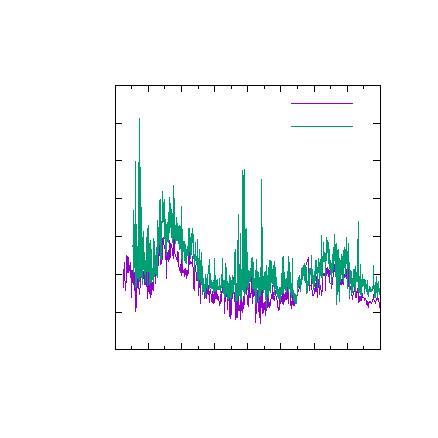
\includegraphics{../images/correlation_ts02}}%
    \gplfronttext
  \end{picture}%
\endgroup

  \caption{Time series of the \ch{NO} concentration during the two
    measurements on January 22 and January 25. Green depicts the
    chemiluminescence measurement, violet the ICAD measurement.}
  \label{fig:corr-ts}
\end{figure}
\begin{figure}[htbp]
  \centering
  % GNUPLOT: LaTeX picture with Postscript
\begingroup
  \makeatletter
  \providecommand\color[2][]{%
    \GenericError{(gnuplot) \space\space\space\@spaces}{%
      Package color not loaded in conjunction with
      terminal option `colourtext'%
    }{See the gnuplot documentation for explanation.%
    }{Either use 'blacktext' in gnuplot or load the package
      color.sty in LaTeX.}%
    \renewcommand\color[2][]{}%
  }%
  \providecommand\includegraphics[2][]{%
    \GenericError{(gnuplot) \space\space\space\@spaces}{%
      Package graphicx or graphics not loaded%
    }{See the gnuplot documentation for explanation.%
    }{The gnuplot epslatex terminal needs graphicx.sty or graphics.sty.}%
    \renewcommand\includegraphics[2][]{}%
  }%
  \providecommand\rotatebox[2]{#2}%
  \@ifundefined{ifGPcolor}{%
    \newif\ifGPcolor
    \GPcolorfalse
  }{}%
  \@ifundefined{ifGPblacktext}{%
    \newif\ifGPblacktext
    \GPblacktexttrue
  }{}%
  % define a \g@addto@macro without @ in the name:
  \let\gplgaddtomacro\g@addto@macro
  % define empty templates for all commands taking text:
  \gdef\gplbacktext{}%
  \gdef\gplfronttext{}%
  \makeatother
  \ifGPblacktext
    % no textcolor at all
    \def\colorrgb#1{}%
    \def\colorgray#1{}%
  \else
    % gray or color?
    \ifGPcolor
      \def\colorrgb#1{\color[rgb]{#1}}%
      \def\colorgray#1{\color[gray]{#1}}%
      \expandafter\def\csname LTw\endcsname{\color{white}}%
      \expandafter\def\csname LTb\endcsname{\color{black}}%
      \expandafter\def\csname LTa\endcsname{\color{black}}%
      \expandafter\def\csname LT0\endcsname{\color[rgb]{1,0,0}}%
      \expandafter\def\csname LT1\endcsname{\color[rgb]{0,1,0}}%
      \expandafter\def\csname LT2\endcsname{\color[rgb]{0,0,1}}%
      \expandafter\def\csname LT3\endcsname{\color[rgb]{1,0,1}}%
      \expandafter\def\csname LT4\endcsname{\color[rgb]{0,1,1}}%
      \expandafter\def\csname LT5\endcsname{\color[rgb]{1,1,0}}%
      \expandafter\def\csname LT6\endcsname{\color[rgb]{0,0,0}}%
      \expandafter\def\csname LT7\endcsname{\color[rgb]{1,0.3,0}}%
      \expandafter\def\csname LT8\endcsname{\color[rgb]{0.5,0.5,0.5}}%
    \else
      % gray
      \def\colorrgb#1{\color{black}}%
      \def\colorgray#1{\color[gray]{#1}}%
      \expandafter\def\csname LTw\endcsname{\color{white}}%
      \expandafter\def\csname LTb\endcsname{\color{black}}%
      \expandafter\def\csname LTa\endcsname{\color{black}}%
      \expandafter\def\csname LT0\endcsname{\color{black}}%
      \expandafter\def\csname LT1\endcsname{\color{black}}%
      \expandafter\def\csname LT2\endcsname{\color{black}}%
      \expandafter\def\csname LT3\endcsname{\color{black}}%
      \expandafter\def\csname LT4\endcsname{\color{black}}%
      \expandafter\def\csname LT5\endcsname{\color{black}}%
      \expandafter\def\csname LT6\endcsname{\color{black}}%
      \expandafter\def\csname LT7\endcsname{\color{black}}%
      \expandafter\def\csname LT8\endcsname{\color{black}}%
    \fi
  \fi
    \setlength{\unitlength}{0.0500bp}%
    \ifx\gptboxheight\undefined%
      \newlength{\gptboxheight}%
      \newlength{\gptboxwidth}%
      \newsavebox{\gptboxtext}%
    \fi%
    \setlength{\fboxrule}{0.5pt}%
    \setlength{\fboxsep}{1pt}%
\begin{picture}(7776.00,4320.00)%
    \gplgaddtomacro\gplbacktext{%
      \csname LTb\endcsname%
      \put(682,704){\makebox(0,0)[r]{\strut{}$-5$}}%
      \put(682,1039){\makebox(0,0)[r]{\strut{}$0$}}%
      \put(682,1374){\makebox(0,0)[r]{\strut{}$5$}}%
      \put(682,1709){\makebox(0,0)[r]{\strut{}$10$}}%
      \put(682,2044){\makebox(0,0)[r]{\strut{}$15$}}%
      \put(682,2380){\makebox(0,0)[r]{\strut{}$20$}}%
      \put(682,2715){\makebox(0,0)[r]{\strut{}$25$}}%
      \put(682,3050){\makebox(0,0)[r]{\strut{}$30$}}%
      \put(682,3385){\makebox(0,0)[r]{\strut{}$35$}}%
      \put(682,3720){\makebox(0,0)[r]{\strut{}$40$}}%
      \put(682,4055){\makebox(0,0)[r]{\strut{}$45$}}%
      \put(814,484){\makebox(0,0){\strut{}$-5$}}%
      \put(1752,484){\makebox(0,0){\strut{}$0$}}%
      \put(2690,484){\makebox(0,0){\strut{}$5$}}%
      \put(3628,484){\makebox(0,0){\strut{}$10$}}%
      \put(4565,484){\makebox(0,0){\strut{}$15$}}%
      \put(5503,484){\makebox(0,0){\strut{}$20$}}%
      \put(6441,484){\makebox(0,0){\strut{}$25$}}%
      \put(7379,484){\makebox(0,0){\strut{}$30$}}%
    }%
    \gplgaddtomacro\gplfronttext{%
      \csname LTb\endcsname%
      \put(176,2379){\rotatebox{-270}{\makebox(0,0){\strut{}Concentration (CLD) [ppb]}}}%
      \put(4096,154){\makebox(0,0){\strut{}Concentration (ICAD) [ppb]}}%
      \csname LTb\endcsname%
      \put(3322,3882){\makebox(0,0)[r]{\strut{}uncorrected}}%
      \csname LTb\endcsname%
      \put(3322,3662){\makebox(0,0)[r]{\strut{}fit uncorrected}}%
      \csname LTb\endcsname%
      \put(3322,3442){\makebox(0,0)[r]{\strut{}tail corrected}}%
      \csname LTb\endcsname%
      \put(3322,3222){\makebox(0,0)[r]{\strut{}fit tail corrected}}%
    }%
    \gplbacktext
    \put(0,0){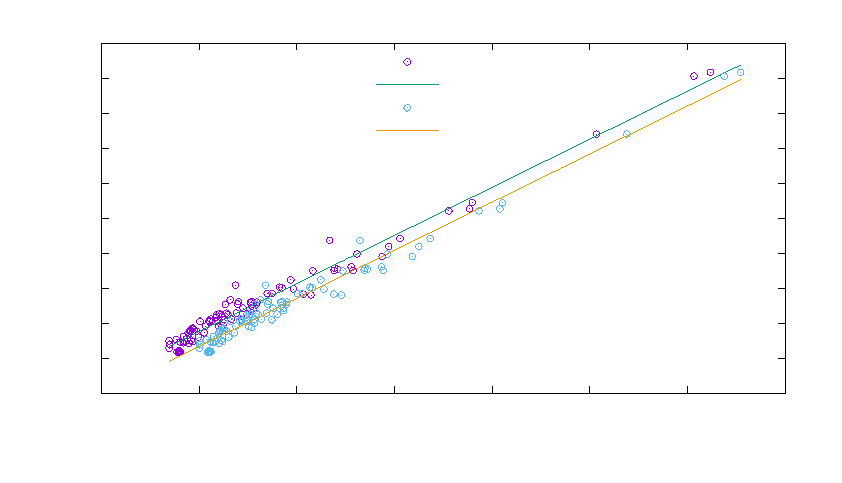
\includegraphics{../images/Correlation_corrected}}%
    \gplfronttext
  \end{picture}%
\endgroup

  \caption{Correlation plot between the \ch{NO_x} ICAD instrument and
    a chemiluminescence monitor (CLD). Each data point depicts a
    \SI{30}{\minute} average.}
  \label{fig:cld-corr}
\end{figure}

All in all it seems that there are a few more stumbling blocks ahead
before this alternating measurement mode is ready for productive
use. The behavior of the converter after an ozone switch has to be
characterized thoroughly to explain and cope with all the observed
effects.

%%% Local Variables:
%%% mode: latex
%%% TeX-master: "../Bachelor"
%%% End:

\subsection{Vehicle measurements}
\label{sec:vehicle}

During this last measurement, we wanted to test our converter under
the conditions of in vivo vehicle measurements. The great advantage in
this setting is, that all European guidelines for Nitrogen Oxide
emission only talk about \ch{NO_x} (c.\,f.~\cite{eu}), i.\,e.\ in this
case we do not need to separate \ch{NO2} from \ch{NO}. Still we wanted
to compare our \ch{NO_x} results to the results of pure \ch{NO2}
measurements to gauge the influence of the additional \ch{NO} on the
air pollution. Therefore we decided to use two cavities in
parallel. One with our converter, the other one without. With this
very comfortable setup, we could even compute the \ch{NO}
concentration without having to switch the Ozone, which mitigated all
the undesired effects described in the previous two sections.

\subsubsection{Setup}
\label{sec:vehicle-setup}

For the measurement we loaded a car (Ford Focus) with both cavities
and positioned the pickup tube directly above the front license
plate. The \ch{NO_x} cavity was setup according to
Section~\ref{sec:inclusion} with an exposure time of
\SI{10}{\milli\second} and 1000 scans per spectrum leading to a time
resolution of \SI{1}{\second}. As \ch{NO2}
cavity we used the AQM$_{\text{Tec}}$ Compact Cavity, which is the
standard cavity at the Institute for Environmental Physics for
measurements in urban areas and especially vehicle measurements. This
cavity operated at a \SI{2}{\second} timely resolution. The
measurement took place on Friday, February 05, 2016 in Heidelberg
between 11:00 and 16:30. From 12:15 to 13:45, we operated both
cavities in \ch{NO2} mode to test for systematic deviations. From
15:00 to 16:15, we positioned our measurement car next to the
Heidelberg air quality measurement station to be able to compare our
\ch{NO} and \ch{NO2} values to the ones of the station as a measure of
reliability. In between we followed various vehicles throughout
Heidelberg between {\nfrac{} 1/2}~\si{\minute} and \SI{10}{\minute}
and tried to stay within their exhaust plume. Since the two cavities's
clocks could not be fully synchronized, the timeseries had to be
matched in the evaluation step. This was done manually using succinct
peaks in the plots.
\todo{write something about \ch{CO2}}

\begin{figure}[htbp]
  \centering
  % GNUPLOT: LaTeX picture with Postscript
\begingroup
  \makeatletter
  \providecommand\color[2][]{%
    \GenericError{(gnuplot) \space\space\space\@spaces}{%
      Package color not loaded in conjunction with
      terminal option `colourtext'%
    }{See the gnuplot documentation for explanation.%
    }{Either use 'blacktext' in gnuplot or load the package
      color.sty in LaTeX.}%
    \renewcommand\color[2][]{}%
  }%
  \providecommand\includegraphics[2][]{%
    \GenericError{(gnuplot) \space\space\space\@spaces}{%
      Package graphicx or graphics not loaded%
    }{See the gnuplot documentation for explanation.%
    }{The gnuplot epslatex terminal needs graphicx.sty or graphics.sty.}%
    \renewcommand\includegraphics[2][]{}%
  }%
  \providecommand\rotatebox[2]{#2}%
  \@ifundefined{ifGPcolor}{%
    \newif\ifGPcolor
    \GPcolorfalse
  }{}%
  \@ifundefined{ifGPblacktext}{%
    \newif\ifGPblacktext
    \GPblacktexttrue
  }{}%
  % define a \g@addto@macro without @ in the name:
  \let\gplgaddtomacro\g@addto@macro
  % define empty templates for all commands taking text:
  \gdef\gplbacktext{}%
  \gdef\gplfronttext{}%
  \makeatother
  \ifGPblacktext
    % no textcolor at all
    \def\colorrgb#1{}%
    \def\colorgray#1{}%
  \else
    % gray or color?
    \ifGPcolor
      \def\colorrgb#1{\color[rgb]{#1}}%
      \def\colorgray#1{\color[gray]{#1}}%
      \expandafter\def\csname LTw\endcsname{\color{white}}%
      \expandafter\def\csname LTb\endcsname{\color{black}}%
      \expandafter\def\csname LTa\endcsname{\color{black}}%
      \expandafter\def\csname LT0\endcsname{\color[rgb]{1,0,0}}%
      \expandafter\def\csname LT1\endcsname{\color[rgb]{0,1,0}}%
      \expandafter\def\csname LT2\endcsname{\color[rgb]{0,0,1}}%
      \expandafter\def\csname LT3\endcsname{\color[rgb]{1,0,1}}%
      \expandafter\def\csname LT4\endcsname{\color[rgb]{0,1,1}}%
      \expandafter\def\csname LT5\endcsname{\color[rgb]{1,1,0}}%
      \expandafter\def\csname LT6\endcsname{\color[rgb]{0,0,0}}%
      \expandafter\def\csname LT7\endcsname{\color[rgb]{1,0.3,0}}%
      \expandafter\def\csname LT8\endcsname{\color[rgb]{0.5,0.5,0.5}}%
    \else
      % gray
      \def\colorrgb#1{\color{black}}%
      \def\colorgray#1{\color[gray]{#1}}%
      \expandafter\def\csname LTw\endcsname{\color{white}}%
      \expandafter\def\csname LTb\endcsname{\color{black}}%
      \expandafter\def\csname LTa\endcsname{\color{black}}%
      \expandafter\def\csname LT0\endcsname{\color{black}}%
      \expandafter\def\csname LT1\endcsname{\color{black}}%
      \expandafter\def\csname LT2\endcsname{\color{black}}%
      \expandafter\def\csname LT3\endcsname{\color{black}}%
      \expandafter\def\csname LT4\endcsname{\color{black}}%
      \expandafter\def\csname LT5\endcsname{\color{black}}%
      \expandafter\def\csname LT6\endcsname{\color{black}}%
      \expandafter\def\csname LT7\endcsname{\color{black}}%
      \expandafter\def\csname LT8\endcsname{\color{black}}%
    \fi
  \fi
    \setlength{\unitlength}{0.0500bp}%
    \ifx\gptboxheight\undefined%
      \newlength{\gptboxheight}%
      \newlength{\gptboxwidth}%
      \newsavebox{\gptboxtext}%
    \fi%
    \setlength{\fboxrule}{0.5pt}%
    \setlength{\fboxsep}{1pt}%
\begin{picture}(7776.00,4320.00)%
    \gplgaddtomacro\gplbacktext{%
      \csname LTb\endcsname%
      \put(682,440){\makebox(0,0)[r]{\strut{}$10$}}%
      \put(682,892){\makebox(0,0)[r]{\strut{}$20$}}%
      \put(682,1344){\makebox(0,0)[r]{\strut{}$30$}}%
      \put(682,1796){\makebox(0,0)[r]{\strut{}$40$}}%
      \put(682,2248){\makebox(0,0)[r]{\strut{}$50$}}%
      \put(682,2699){\makebox(0,0)[r]{\strut{}$60$}}%
      \put(682,3151){\makebox(0,0)[r]{\strut{}$70$}}%
      \put(682,3603){\makebox(0,0)[r]{\strut{}$80$}}%
      \put(682,4055){\makebox(0,0)[r]{\strut{}$90$}}%
      \put(814,220){\makebox(0,0){\strut{}12:10}}%
      \put(1471,220){\makebox(0,0){\strut{}12:20}}%
      \put(2127,220){\makebox(0,0){\strut{}12:30}}%
      \put(2784,220){\makebox(0,0){\strut{}12:40}}%
      \put(3440,220){\makebox(0,0){\strut{}12:50}}%
      \put(4097,220){\makebox(0,0){\strut{}13:00}}%
      \put(4753,220){\makebox(0,0){\strut{}13:10}}%
      \put(5410,220){\makebox(0,0){\strut{}13:20}}%
      \put(6066,220){\makebox(0,0){\strut{}13:30}}%
      \put(6723,220){\makebox(0,0){\strut{}13:40}}%
      \put(7379,220){\makebox(0,0){\strut{}13:50}}%
    }%
    \gplgaddtomacro\gplfronttext{%
      \csname LTb\endcsname%
      \put(176,2247){\rotatebox{-270}{\makebox(0,0){\strut{}Concentration [ppb]}}}%
      \csname LTb\endcsname%
      \put(6392,3882){\makebox(0,0)[r]{\strut{}\text{\ch{NO2} of ICAD \ch{NO2} CE-DOAS}}}%
      \csname LTb\endcsname%
      \put(6392,3662){\makebox(0,0)[r]{\strut{}\text{\ch{NO2} of ICAD \ch{NO_x} CE-DOAS}}}%
    }%
    \gplbacktext
    \put(0,0){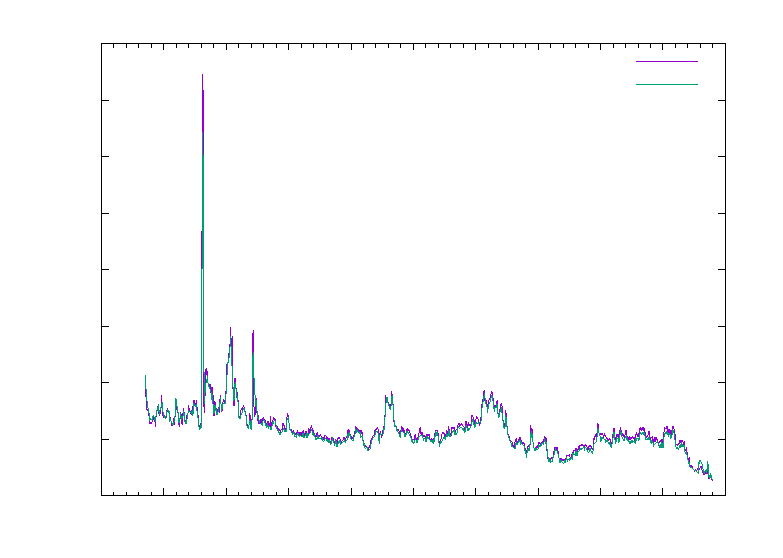
\includegraphics{../images/hd_comparison}}%
    \gplfronttext
  \end{picture}%
\endgroup

  \caption{Comparison of the two used CE-DOAS systems. Both were
    operated in pure \ch{NO2} measurement mode. The difference is
    \SI{0.43 \pm 0.01}{ppb}.}
  \label{fig:hd-comparison}
\end{figure}

\subsubsection{Results}
\label{sec:vehicle-results}

In Figure~\ref{fig:hd-comparison} you can see the comparison of the
measured \ch{NO2} concentrations of the two used cavities. It is
clearly visible that ther is no qualitative difference between the
two. However, our \ch{NO_x} cavity measures slightly lower
concentrations than the \ch{NO2} cavity with a mean difference of
$\Delta = \SI{0.43\pm0.01}{ppb}$. Absolutely speaking this is not a
large difference, but the question remains why it shows up at all. The
most probable explanation is that the used zero air spectrum of the
\ch{NO_x} cavity was not completely trace gas free. On reason that
points towards this direction is, that in the \ch{NO_x} measurement
mode, we have a constant flow through the zero air input, as this is
the input for the Ozone generator. Thus the zero air filters are much
more strained than they would be in a cavity without \ch{NO_x}
mode. Additionally the cavity had been thoroughly tested for multiple
weeks, such that a saturation or starting effects of a saturation of
the Silica gel or the activated carbon seem plausible. 

\begin{figure}[htbp]
  \centering
  % GNUPLOT: LaTeX picture with Postscript
\begingroup
  \makeatletter
  \providecommand\color[2][]{%
    \GenericError{(gnuplot) \space\space\space\@spaces}{%
      Package color not loaded in conjunction with
      terminal option `colourtext'%
    }{See the gnuplot documentation for explanation.%
    }{Either use 'blacktext' in gnuplot or load the package
      color.sty in LaTeX.}%
    \renewcommand\color[2][]{}%
  }%
  \providecommand\includegraphics[2][]{%
    \GenericError{(gnuplot) \space\space\space\@spaces}{%
      Package graphicx or graphics not loaded%
    }{See the gnuplot documentation for explanation.%
    }{The gnuplot epslatex terminal needs graphicx.sty or graphics.sty.}%
    \renewcommand\includegraphics[2][]{}%
  }%
  \providecommand\rotatebox[2]{#2}%
  \@ifundefined{ifGPcolor}{%
    \newif\ifGPcolor
    \GPcolorfalse
  }{}%
  \@ifundefined{ifGPblacktext}{%
    \newif\ifGPblacktext
    \GPblacktexttrue
  }{}%
  % define a \g@addto@macro without @ in the name:
  \let\gplgaddtomacro\g@addto@macro
  % define empty templates for all commands taking text:
  \gdef\gplbacktext{}%
  \gdef\gplfronttext{}%
  \makeatother
  \ifGPblacktext
    % no textcolor at all
    \def\colorrgb#1{}%
    \def\colorgray#1{}%
  \else
    % gray or color?
    \ifGPcolor
      \def\colorrgb#1{\color[rgb]{#1}}%
      \def\colorgray#1{\color[gray]{#1}}%
      \expandafter\def\csname LTw\endcsname{\color{white}}%
      \expandafter\def\csname LTb\endcsname{\color{black}}%
      \expandafter\def\csname LTa\endcsname{\color{black}}%
      \expandafter\def\csname LT0\endcsname{\color[rgb]{1,0,0}}%
      \expandafter\def\csname LT1\endcsname{\color[rgb]{0,1,0}}%
      \expandafter\def\csname LT2\endcsname{\color[rgb]{0,0,1}}%
      \expandafter\def\csname LT3\endcsname{\color[rgb]{1,0,1}}%
      \expandafter\def\csname LT4\endcsname{\color[rgb]{0,1,1}}%
      \expandafter\def\csname LT5\endcsname{\color[rgb]{1,1,0}}%
      \expandafter\def\csname LT6\endcsname{\color[rgb]{0,0,0}}%
      \expandafter\def\csname LT7\endcsname{\color[rgb]{1,0.3,0}}%
      \expandafter\def\csname LT8\endcsname{\color[rgb]{0.5,0.5,0.5}}%
    \else
      % gray
      \def\colorrgb#1{\color{black}}%
      \def\colorgray#1{\color[gray]{#1}}%
      \expandafter\def\csname LTw\endcsname{\color{white}}%
      \expandafter\def\csname LTb\endcsname{\color{black}}%
      \expandafter\def\csname LTa\endcsname{\color{black}}%
      \expandafter\def\csname LT0\endcsname{\color{black}}%
      \expandafter\def\csname LT1\endcsname{\color{black}}%
      \expandafter\def\csname LT2\endcsname{\color{black}}%
      \expandafter\def\csname LT3\endcsname{\color{black}}%
      \expandafter\def\csname LT4\endcsname{\color{black}}%
      \expandafter\def\csname LT5\endcsname{\color{black}}%
      \expandafter\def\csname LT6\endcsname{\color{black}}%
      \expandafter\def\csname LT7\endcsname{\color{black}}%
      \expandafter\def\csname LT8\endcsname{\color{black}}%
    \fi
  \fi
    \setlength{\unitlength}{0.0500bp}%
    \ifx\gptboxheight\undefined%
      \newlength{\gptboxheight}%
      \newlength{\gptboxwidth}%
      \newsavebox{\gptboxtext}%
    \fi%
    \setlength{\fboxrule}{0.5pt}%
    \setlength{\fboxsep}{1pt}%
\begin{picture}(7200.00,5040.00)%
    \gplgaddtomacro\gplbacktext{%
      \csname LTb\endcsname%
      \put(814,440){\makebox(0,0)[r]{\strut{}$-10$}}%
      \put(814,922){\makebox(0,0)[r]{\strut{}$0$}}%
      \put(814,1403){\makebox(0,0)[r]{\strut{}$10$}}%
      \put(814,1885){\makebox(0,0)[r]{\strut{}$20$}}%
      \put(814,2367){\makebox(0,0)[r]{\strut{}$30$}}%
      \put(814,2848){\makebox(0,0)[r]{\strut{}$40$}}%
      \put(814,3330){\makebox(0,0)[r]{\strut{}$50$}}%
      \put(814,3812){\makebox(0,0)[r]{\strut{}$60$}}%
      \put(814,4293){\makebox(0,0)[r]{\strut{}$70$}}%
      \put(814,4775){\makebox(0,0)[r]{\strut{}$80$}}%
      \put(946,220){\makebox(0,0){\strut{}14:50}}%
      \put(1597,220){\makebox(0,0){\strut{}15:00}}%
      \put(2248,220){\makebox(0,0){\strut{}15:10}}%
      \put(2898,220){\makebox(0,0){\strut{}15:20}}%
      \put(3549,220){\makebox(0,0){\strut{}15:30}}%
      \put(4200,220){\makebox(0,0){\strut{}15:40}}%
      \put(4851,220){\makebox(0,0){\strut{}15:50}}%
      \put(5501,220){\makebox(0,0){\strut{}16:00}}%
      \put(6152,220){\makebox(0,0){\strut{}16:10}}%
      \put(6803,220){\makebox(0,0){\strut{}16:20}}%
    }%
    \gplgaddtomacro\gplfronttext{%
      \csname LTb\endcsname%
      \put(176,2607){\rotatebox{-270}{\makebox(0,0){\strut{}Concentration [ppb]}}}%
      \csname LTb\endcsname%
      \put(5816,4602){\makebox(0,0)[r]{\strut{}\ch{NO2}}}%
      \csname LTb\endcsname%
      \put(5816,4382){\makebox(0,0)[r]{\strut{}\ch{NO_x}}}%
      \csname LTb\endcsname%
      \put(5816,4162){\makebox(0,0)[r]{\strut{}\ch{NO_{\text{\hphantom{x}}}}}}%
    }%
    \gplbacktext
    \put(0,0){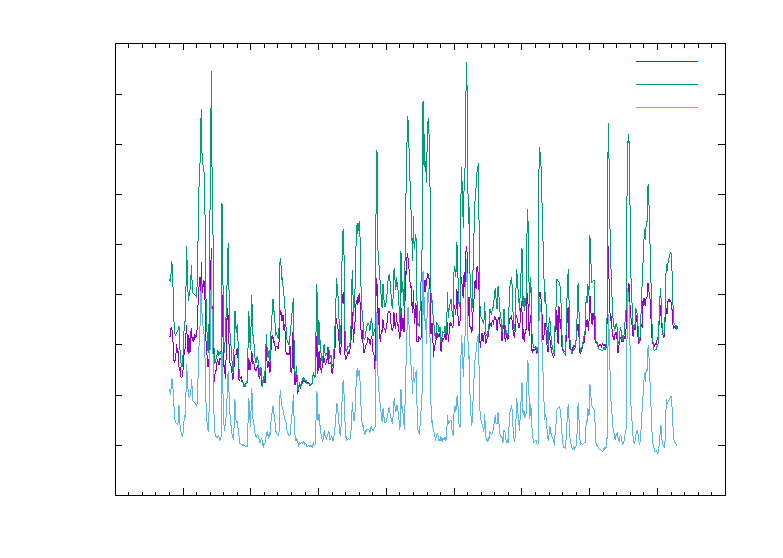
\includegraphics{../images/umba_ts}}%
    \gplfronttext
  \end{picture}%
\endgroup

  \caption{Timeseries of the \ch{NO_x}, \ch{NO2} and the computed
    \ch{NO} concentration next to the Umweltlandesamt air quality
    measurement station in Heidelberg.}
  \label{fig:umba}
\end{figure}

Figure~\ref{fig:umba} contains the timeseries of the measured
\ch{NO_x} and \ch{NO_2} and the computed \ch{NO} during our stay next
to the Heidelberg air quality measurement station. This time series is
representative for all the measurements we took that day. For moderate
\ch{NO2} concentrations between \num{10} and \SI{20}{ppb} the
\ch{NO_x} curve almost coincides with the \ch{NO2} curve. Only during
peaks we have a stronger separation and the \ch{NO_x} concentration
rises occasionally twice as high as the \ch{NO2} concentration. The
time series makes clear that neglecting \ch{NO} values while
estimating \ch{NO_x} pollution in urban areas can lead to
underestimation.

In a next step we computed the average concentrations for all three
time series and compared them to the station data taken
from~\cite{umba}. The results can be found in Table~\ref{tab:umba}. We
see that we have a systematic deviation from the station values,
but our values lie in the same region. The standard CE-DOAS method has
been thoroughly tested during the last decades and is known to produce
solid results ind good accordance with the measurement station. Thus
the deviation of the \ch{NO2} averages already points towards outer
influences, which can explain the deviations. Indeed our pickup tube
was about \SI{3}{\meter} away from the station inlet and approximately
\SI{1}{\meter} lower (which means also closer to the driving
surface). These differences in exact location can easily account for
our measured derivations.

Nevertheless, the main result stays that under field conditions in
ambient air our measured \ch{NO_x} or respectively computed \ch{NO}
values are comparable to the ones of the station, thus indicating once
more that our converter together with a second cavity seem to work as
a good setup for \ch{NO} measurements. Still some more (and longer)
measurements would be advisable to aquire more data points for enough
statistics to make a comparison between the DOAS method and other
established \ch{NO} measurement methods resilient.

\begin{table}[htbp]
  \centering
  \sisetup{
    table-format=2.1(2)
  }
  \begin{tabular}{l S S}
    \toprule
    {Compound} & \multicolumn{2}{c}{Concentration in \si{ppb}}\\
    & {Station} & {DOAS}\\
    \midrule
    \ch{NO} & 7.4 & 6.5 \pm 0.2\\
    \ch{NO2} & 19.2 & 21.9 \pm 0.1\\
    \ch{NOx} & 26.6 & 28.2 \pm 0.4\\ 
    \bottomrule
  \end{tabular}
  \caption{Comparison of the \SI{1}{\hour} \ch{NO}, \ch{NO2} and
    \ch{NO_x} averages from 15:00 to 16:00 on February 05, 2016
    between the air quality measurement station and the improved CE-DOAS
    instrument. The station data was taken from~\cite{umba}; no
    uncertainties were provided.}
  \label{tab:umba}
\end{table}

\begin{figure}[htbp]
  \centering
  % GNUPLOT: LaTeX picture with Postscript
\begingroup
  \makeatletter
  \providecommand\color[2][]{%
    \GenericError{(gnuplot) \space\space\space\@spaces}{%
      Package color not loaded in conjunction with
      terminal option `colourtext'%
    }{See the gnuplot documentation for explanation.%
    }{Either use 'blacktext' in gnuplot or load the package
      color.sty in LaTeX.}%
    \renewcommand\color[2][]{}%
  }%
  \providecommand\includegraphics[2][]{%
    \GenericError{(gnuplot) \space\space\space\@spaces}{%
      Package graphicx or graphics not loaded%
    }{See the gnuplot documentation for explanation.%
    }{The gnuplot epslatex terminal needs graphicx.sty or graphics.sty.}%
    \renewcommand\includegraphics[2][]{}%
  }%
  \providecommand\rotatebox[2]{#2}%
  \@ifundefined{ifGPcolor}{%
    \newif\ifGPcolor
    \GPcolorfalse
  }{}%
  \@ifundefined{ifGPblacktext}{%
    \newif\ifGPblacktext
    \GPblacktexttrue
  }{}%
  % define a \g@addto@macro without @ in the name:
  \let\gplgaddtomacro\g@addto@macro
  % define empty templates for all commands taking text:
  \gdef\gplbacktext{}%
  \gdef\gplfronttext{}%
  \makeatother
  \ifGPblacktext
    % no textcolor at all
    \def\colorrgb#1{}%
    \def\colorgray#1{}%
  \else
    % gray or color?
    \ifGPcolor
      \def\colorrgb#1{\color[rgb]{#1}}%
      \def\colorgray#1{\color[gray]{#1}}%
      \expandafter\def\csname LTw\endcsname{\color{white}}%
      \expandafter\def\csname LTb\endcsname{\color{black}}%
      \expandafter\def\csname LTa\endcsname{\color{black}}%
      \expandafter\def\csname LT0\endcsname{\color[rgb]{1,0,0}}%
      \expandafter\def\csname LT1\endcsname{\color[rgb]{0,1,0}}%
      \expandafter\def\csname LT2\endcsname{\color[rgb]{0,0,1}}%
      \expandafter\def\csname LT3\endcsname{\color[rgb]{1,0,1}}%
      \expandafter\def\csname LT4\endcsname{\color[rgb]{0,1,1}}%
      \expandafter\def\csname LT5\endcsname{\color[rgb]{1,1,0}}%
      \expandafter\def\csname LT6\endcsname{\color[rgb]{0,0,0}}%
      \expandafter\def\csname LT7\endcsname{\color[rgb]{1,0.3,0}}%
      \expandafter\def\csname LT8\endcsname{\color[rgb]{0.5,0.5,0.5}}%
    \else
      % gray
      \def\colorrgb#1{\color{black}}%
      \def\colorgray#1{\color[gray]{#1}}%
      \expandafter\def\csname LTw\endcsname{\color{white}}%
      \expandafter\def\csname LTb\endcsname{\color{black}}%
      \expandafter\def\csname LTa\endcsname{\color{black}}%
      \expandafter\def\csname LT0\endcsname{\color{black}}%
      \expandafter\def\csname LT1\endcsname{\color{black}}%
      \expandafter\def\csname LT2\endcsname{\color{black}}%
      \expandafter\def\csname LT3\endcsname{\color{black}}%
      \expandafter\def\csname LT4\endcsname{\color{black}}%
      \expandafter\def\csname LT5\endcsname{\color{black}}%
      \expandafter\def\csname LT6\endcsname{\color{black}}%
      \expandafter\def\csname LT7\endcsname{\color{black}}%
      \expandafter\def\csname LT8\endcsname{\color{black}}%
    \fi
  \fi
    \setlength{\unitlength}{0.0500bp}%
    \ifx\gptboxheight\undefined%
      \newlength{\gptboxheight}%
      \newlength{\gptboxwidth}%
      \newsavebox{\gptboxtext}%
    \fi%
    \setlength{\fboxrule}{0.5pt}%
    \setlength{\fboxsep}{1pt}%
\begin{picture}(7200.00,5040.00)%
    \gplgaddtomacro\gplbacktext{%
      \csname LTb\endcsname%
      \put(946,966){\makebox(0,0)[r]{\strut{}$0$}}%
      \put(946,1389){\makebox(0,0)[r]{\strut{}$500$}}%
      \put(946,1812){\makebox(0,0)[r]{\strut{}$1000$}}%
      \put(946,2236){\makebox(0,0)[r]{\strut{}$1500$}}%
      \put(946,2659){\makebox(0,0)[r]{\strut{}$2000$}}%
      \put(946,3082){\makebox(0,0)[r]{\strut{}$2500$}}%
      \put(946,3505){\makebox(0,0)[r]{\strut{}$3000$}}%
      \put(946,3929){\makebox(0,0)[r]{\strut{}$3500$}}%
      \put(946,4352){\makebox(0,0)[r]{\strut{}$4000$}}%
      \put(946,4775){\makebox(0,0)[r]{\strut{}$4500$}}%
      \put(1078,834){\rotatebox{-45}{\makebox(0,0)[l]{\strut{}14:25:00}}}%
      \put(1549,834){\rotatebox{-45}{\makebox(0,0)[l]{\strut{}14:26:00}}}%
      \put(2021,834){\rotatebox{-45}{\makebox(0,0)[l]{\strut{}14:27:00}}}%
      \put(2492,834){\rotatebox{-45}{\makebox(0,0)[l]{\strut{}14:28:00}}}%
      \put(2963,834){\rotatebox{-45}{\makebox(0,0)[l]{\strut{}14:29:00}}}%
      \put(3435,834){\rotatebox{-45}{\makebox(0,0)[l]{\strut{}14:30:00}}}%
      \put(3906,834){\rotatebox{-45}{\makebox(0,0)[l]{\strut{}14:31:00}}}%
      \put(4377,834){\rotatebox{-45}{\makebox(0,0)[l]{\strut{}14:32:00}}}%
      \put(4848,834){\rotatebox{-45}{\makebox(0,0)[l]{\strut{}14:33:00}}}%
      \put(5320,834){\rotatebox{-45}{\makebox(0,0)[l]{\strut{}14:34:00}}}%
      \put(5791,834){\rotatebox{-45}{\makebox(0,0)[l]{\strut{}14:35:00}}}%
      \put(5923,966){\makebox(0,0)[l]{\strut{}$0$}}%
      \put(5923,1389){\makebox(0,0)[l]{\strut{}$500$}}%
      \put(5923,1812){\makebox(0,0)[l]{\strut{}$1000$}}%
      \put(5923,2236){\makebox(0,0)[l]{\strut{}$1500$}}%
      \put(5923,2659){\makebox(0,0)[l]{\strut{}$2000$}}%
      \put(5923,3082){\makebox(0,0)[l]{\strut{}$2500$}}%
      \put(5923,3505){\makebox(0,0)[l]{\strut{}$3000$}}%
      \put(5923,3929){\makebox(0,0)[l]{\strut{}$3500$}}%
      \put(5923,4352){\makebox(0,0)[l]{\strut{}$4000$}}%
      \put(5923,4775){\makebox(0,0)[l]{\strut{}$4500$}}%
    }%
    \gplgaddtomacro\gplfronttext{%
      \csname LTb\endcsname%
      \put(176,2870){\rotatebox{-270}{\makebox(0,0){\strut{}\ch{NO2}/\ch{NO_x} Concentration [ppb]}}}%
      \put(6692,2870){\rotatebox{-270}{\makebox(0,0){\strut{}\ch{CO2} Concentration [ppm]}}}%
      \csname LTb\endcsname%
      \put(1738,4602){\makebox(0,0)[r]{\strut{}\ch{NO2}}}%
      \csname LTb\endcsname%
      \put(1738,4382){\makebox(0,0)[r]{\strut{}\ch{NO_x}}}%
      \csname LTb\endcsname%
      \put(1738,4162){\makebox(0,0)[r]{\strut{}\ch{CO2}}}%
    }%
    \gplbacktext
    \put(0,0){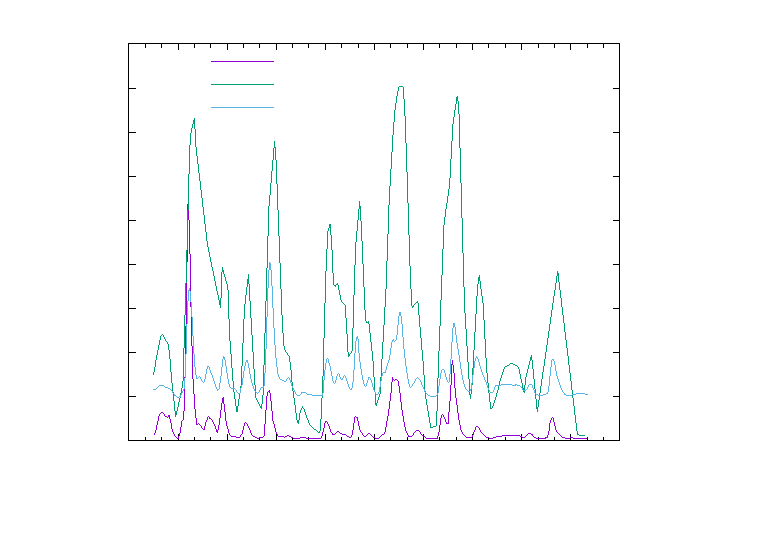
\includegraphics{../images/bus}}%
    \gplfronttext
  \end{picture}%
\endgroup

  \caption{Timeseries of the uncorrected \ch{NO2}, \ch{NO_x} and \ch{CO2}
    concentrations in the plume of a bus in Heidelberg.}
  \label{fig:bus-ts}
\end{figure}

\begin{figure}[htbp]
  \centering
  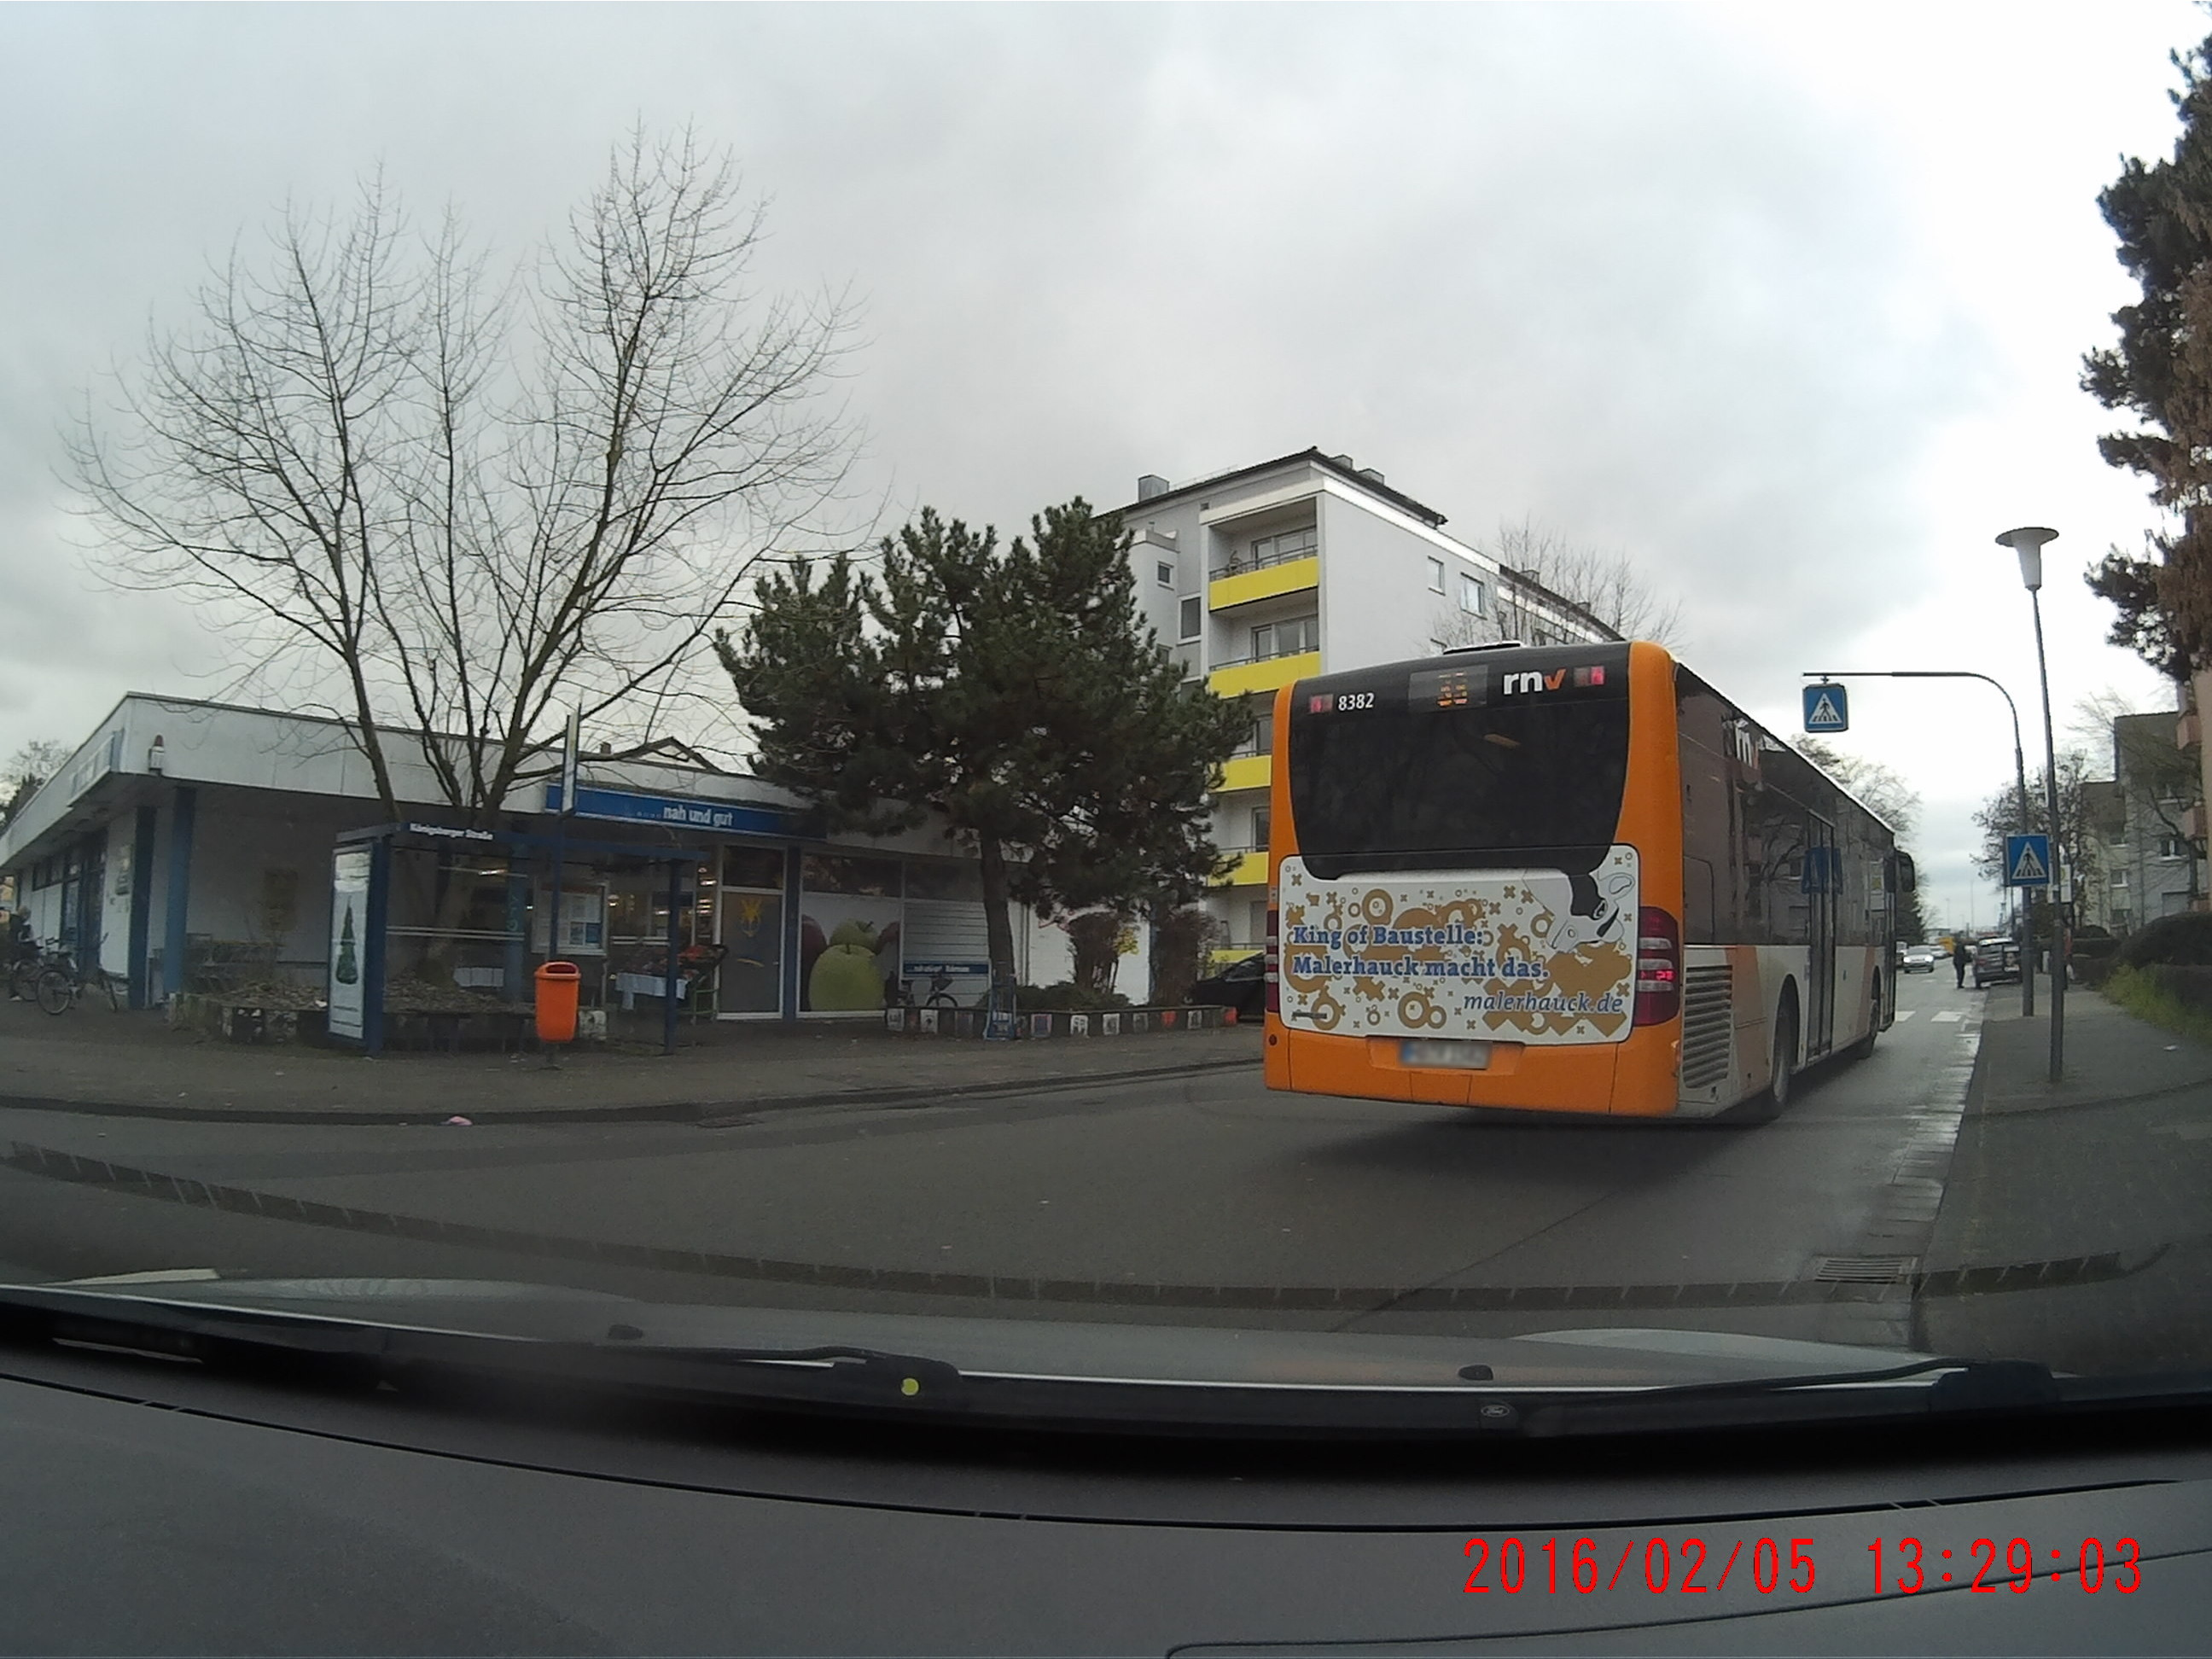
\includegraphics[width=0.45\textwidth]{bus.jpg}
  \hfill
  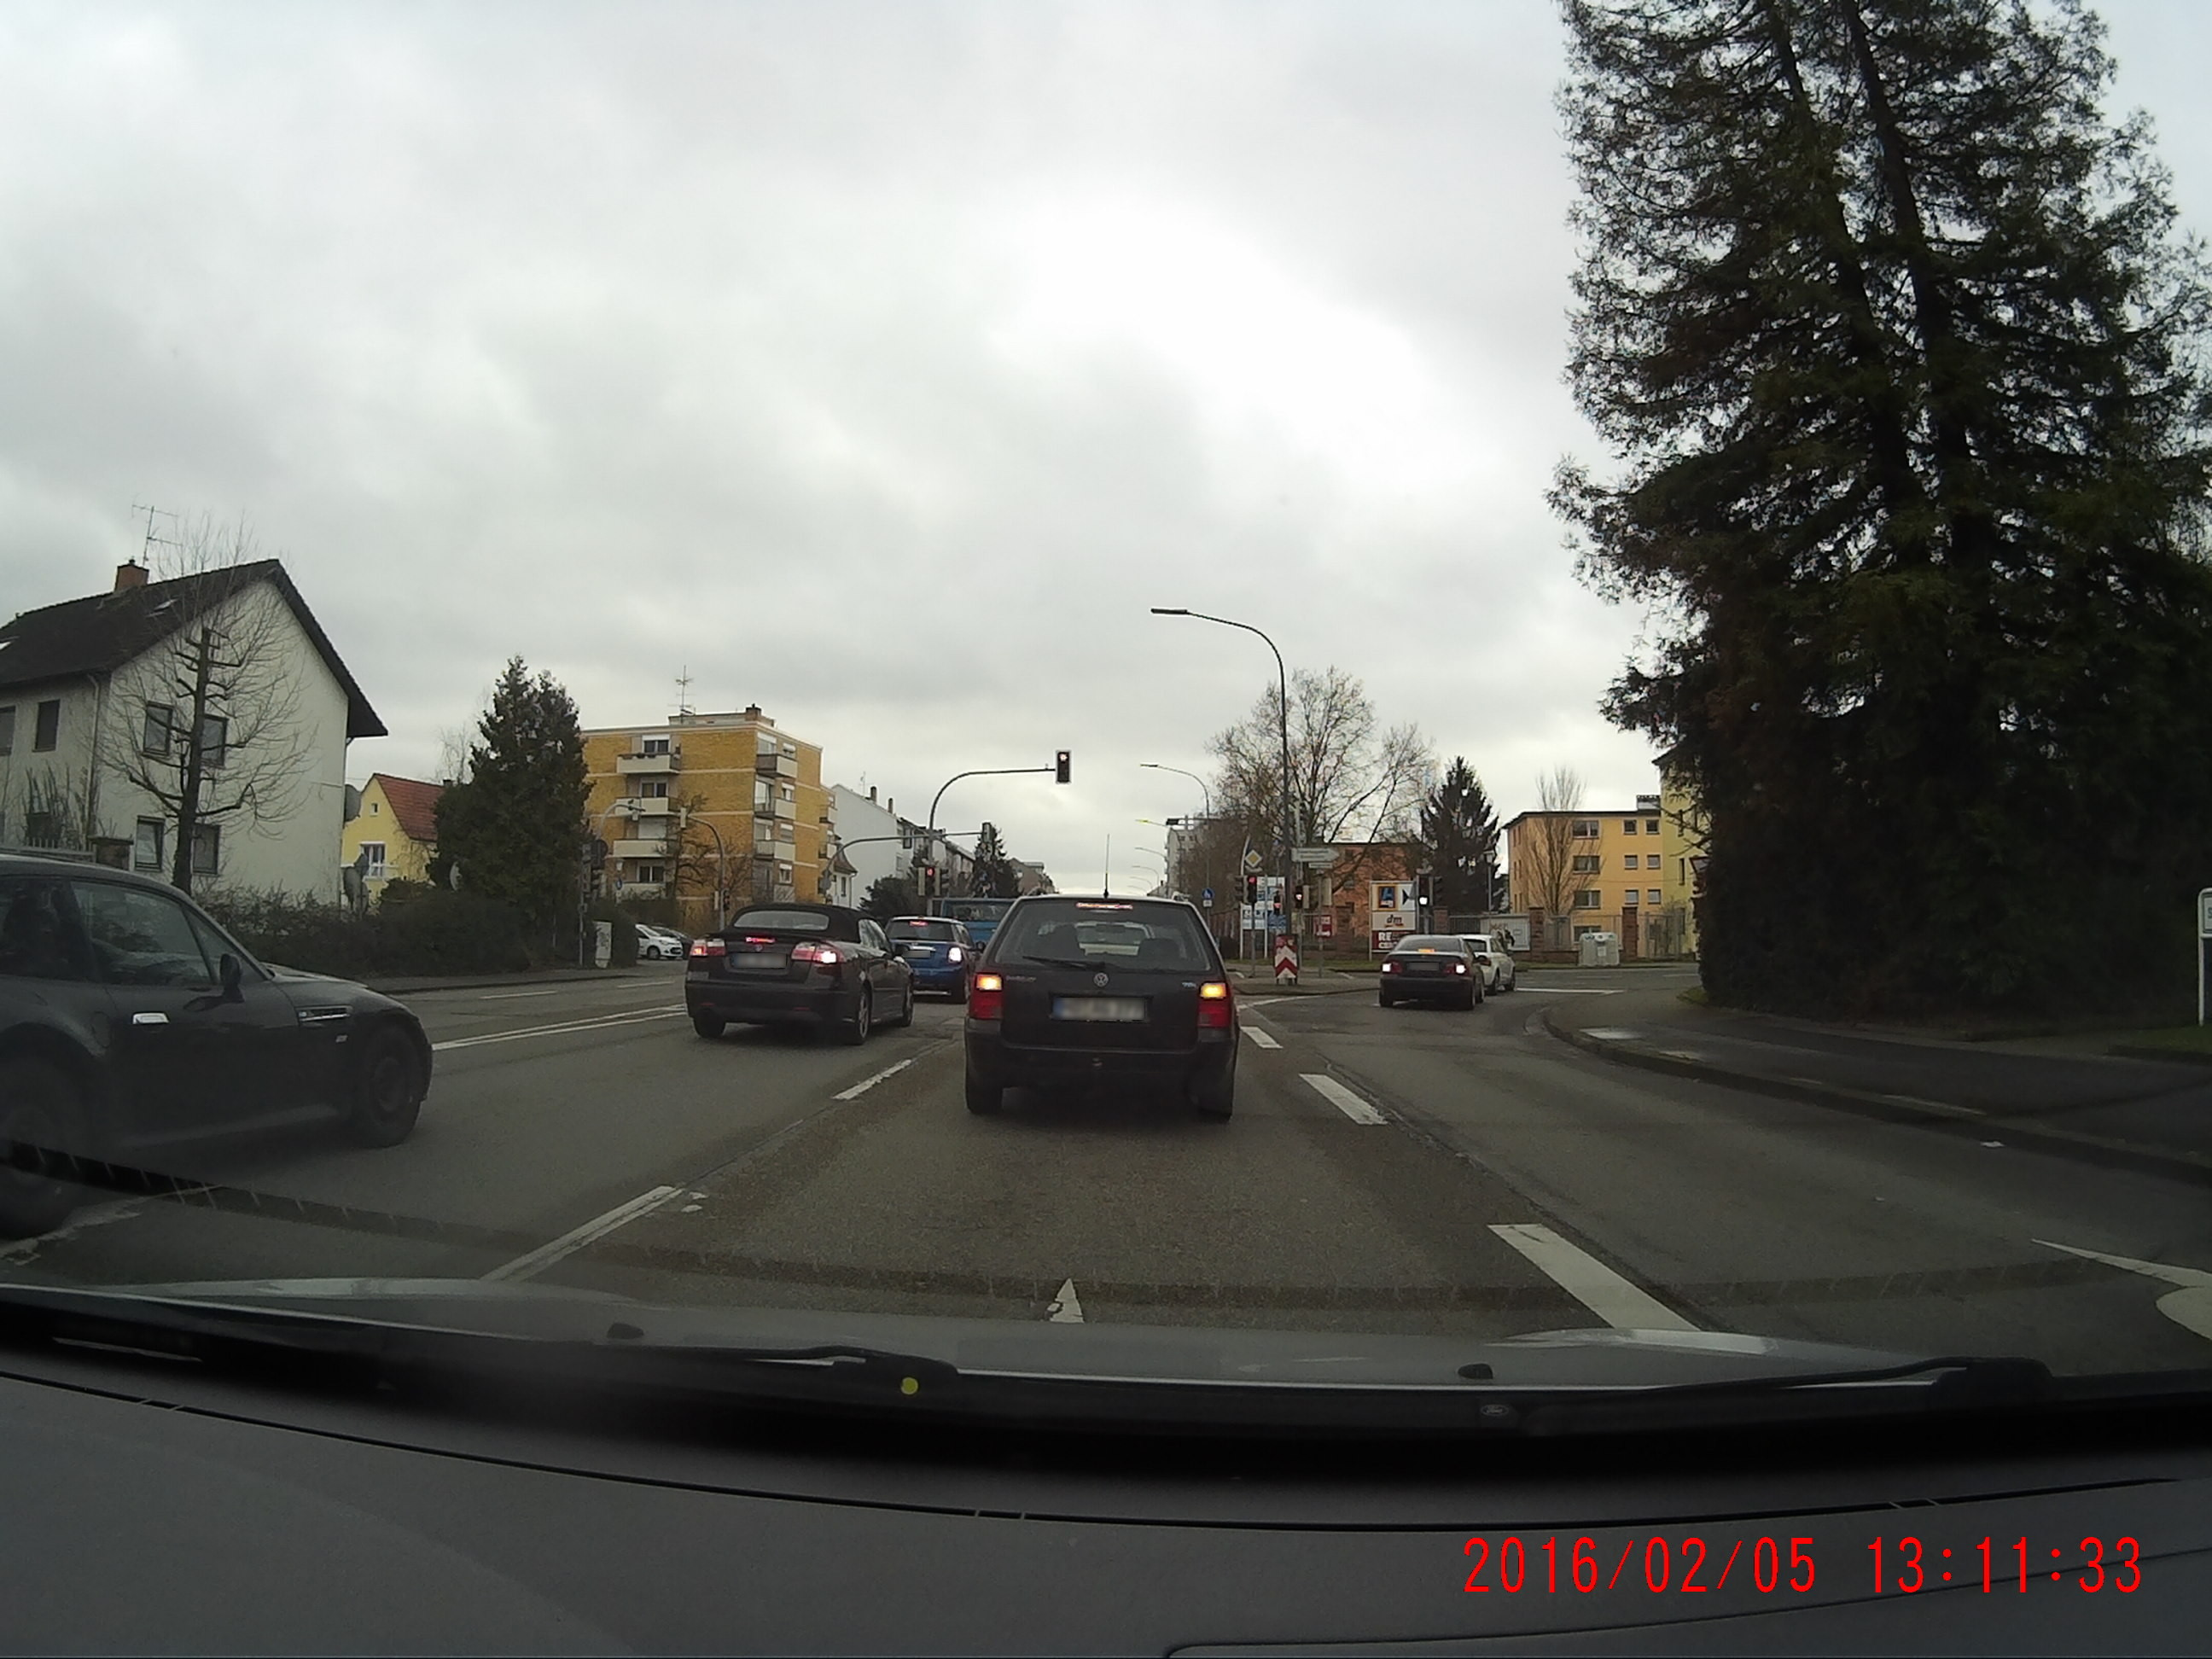
\includegraphics[width=0.45\textwidth]{vw.jpg}
  \caption{Picture of the measured bus and VW Pasat.}
  \label{fig:bus}
\end{figure}

\begin{figure}[htbp]
  \centering
  % GNUPLOT: LaTeX picture with Postscript
\begingroup
  \makeatletter
  \providecommand\color[2][]{%
    \GenericError{(gnuplot) \space\space\space\@spaces}{%
      Package color not loaded in conjunction with
      terminal option `colourtext'%
    }{See the gnuplot documentation for explanation.%
    }{Either use 'blacktext' in gnuplot or load the package
      color.sty in LaTeX.}%
    \renewcommand\color[2][]{}%
  }%
  \providecommand\includegraphics[2][]{%
    \GenericError{(gnuplot) \space\space\space\@spaces}{%
      Package graphicx or graphics not loaded%
    }{See the gnuplot documentation for explanation.%
    }{The gnuplot epslatex terminal needs graphicx.sty or graphics.sty.}%
    \renewcommand\includegraphics[2][]{}%
  }%
  \providecommand\rotatebox[2]{#2}%
  \@ifundefined{ifGPcolor}{%
    \newif\ifGPcolor
    \GPcolorfalse
  }{}%
  \@ifundefined{ifGPblacktext}{%
    \newif\ifGPblacktext
    \GPblacktexttrue
  }{}%
  % define a \g@addto@macro without @ in the name:
  \let\gplgaddtomacro\g@addto@macro
  % define empty templates for all commands taking text:
  \gdef\gplbacktext{}%
  \gdef\gplfronttext{}%
  \makeatother
  \ifGPblacktext
    % no textcolor at all
    \def\colorrgb#1{}%
    \def\colorgray#1{}%
  \else
    % gray or color?
    \ifGPcolor
      \def\colorrgb#1{\color[rgb]{#1}}%
      \def\colorgray#1{\color[gray]{#1}}%
      \expandafter\def\csname LTw\endcsname{\color{white}}%
      \expandafter\def\csname LTb\endcsname{\color{black}}%
      \expandafter\def\csname LTa\endcsname{\color{black}}%
      \expandafter\def\csname LT0\endcsname{\color[rgb]{1,0,0}}%
      \expandafter\def\csname LT1\endcsname{\color[rgb]{0,1,0}}%
      \expandafter\def\csname LT2\endcsname{\color[rgb]{0,0,1}}%
      \expandafter\def\csname LT3\endcsname{\color[rgb]{1,0,1}}%
      \expandafter\def\csname LT4\endcsname{\color[rgb]{0,1,1}}%
      \expandafter\def\csname LT5\endcsname{\color[rgb]{1,1,0}}%
      \expandafter\def\csname LT6\endcsname{\color[rgb]{0,0,0}}%
      \expandafter\def\csname LT7\endcsname{\color[rgb]{1,0.3,0}}%
      \expandafter\def\csname LT8\endcsname{\color[rgb]{0.5,0.5,0.5}}%
    \else
      % gray
      \def\colorrgb#1{\color{black}}%
      \def\colorgray#1{\color[gray]{#1}}%
      \expandafter\def\csname LTw\endcsname{\color{white}}%
      \expandafter\def\csname LTb\endcsname{\color{black}}%
      \expandafter\def\csname LTa\endcsname{\color{black}}%
      \expandafter\def\csname LT0\endcsname{\color{black}}%
      \expandafter\def\csname LT1\endcsname{\color{black}}%
      \expandafter\def\csname LT2\endcsname{\color{black}}%
      \expandafter\def\csname LT3\endcsname{\color{black}}%
      \expandafter\def\csname LT4\endcsname{\color{black}}%
      \expandafter\def\csname LT5\endcsname{\color{black}}%
      \expandafter\def\csname LT6\endcsname{\color{black}}%
      \expandafter\def\csname LT7\endcsname{\color{black}}%
      \expandafter\def\csname LT8\endcsname{\color{black}}%
    \fi
  \fi
    \setlength{\unitlength}{0.0500bp}%
    \ifx\gptboxheight\undefined%
      \newlength{\gptboxheight}%
      \newlength{\gptboxwidth}%
      \newsavebox{\gptboxtext}%
    \fi%
    \setlength{\fboxrule}{0.5pt}%
    \setlength{\fboxsep}{1pt}%
\begin{picture}(7200.00,5040.00)%
    \gplgaddtomacro\gplbacktext{%
      \csname LTb\endcsname%
      \put(814,966){\makebox(0,0)[r]{\strut{}$0$}}%
      \put(814,1389){\makebox(0,0)[r]{\strut{}$100$}}%
      \put(814,1812){\makebox(0,0)[r]{\strut{}$200$}}%
      \put(814,2236){\makebox(0,0)[r]{\strut{}$300$}}%
      \put(814,2659){\makebox(0,0)[r]{\strut{}$400$}}%
      \put(814,3082){\makebox(0,0)[r]{\strut{}$500$}}%
      \put(814,3505){\makebox(0,0)[r]{\strut{}$600$}}%
      \put(814,3929){\makebox(0,0)[r]{\strut{}$700$}}%
      \put(814,4352){\makebox(0,0)[r]{\strut{}$800$}}%
      \put(814,4775){\makebox(0,0)[r]{\strut{}$900$}}%
      \put(946,834){\rotatebox{-45}{\makebox(0,0)[l]{\strut{}14:11:00}}}%
      \put(1776,834){\rotatebox{-45}{\makebox(0,0)[l]{\strut{}14:11:30}}}%
      \put(2605,834){\rotatebox{-45}{\makebox(0,0)[l]{\strut{}14:12:00}}}%
      \put(3435,834){\rotatebox{-45}{\makebox(0,0)[l]{\strut{}14:12:30}}}%
      \put(4264,834){\rotatebox{-45}{\makebox(0,0)[l]{\strut{}14:13:00}}}%
      \put(5094,834){\rotatebox{-45}{\makebox(0,0)[l]{\strut{}14:13:30}}}%
      \put(5923,834){\rotatebox{-45}{\makebox(0,0)[l]{\strut{}14:14:00}}}%
      \put(6055,966){\makebox(0,0)[l]{\strut{}$0$}}%
      \put(6055,1389){\makebox(0,0)[l]{\strut{}$100$}}%
      \put(6055,1812){\makebox(0,0)[l]{\strut{}$200$}}%
      \put(6055,2236){\makebox(0,0)[l]{\strut{}$300$}}%
      \put(6055,2659){\makebox(0,0)[l]{\strut{}$400$}}%
      \put(6055,3082){\makebox(0,0)[l]{\strut{}$500$}}%
      \put(6055,3505){\makebox(0,0)[l]{\strut{}$600$}}%
      \put(6055,3929){\makebox(0,0)[l]{\strut{}$700$}}%
      \put(6055,4352){\makebox(0,0)[l]{\strut{}$800$}}%
      \put(6055,4775){\makebox(0,0)[l]{\strut{}$900$}}%
    }%
    \gplgaddtomacro\gplfronttext{%
      \csname LTb\endcsname%
      \put(176,2870){\rotatebox{-270}{\makebox(0,0){\strut{}\ch{NO2}/\ch{NO_x} Concentration [ppb]}}}%
      \put(6692,2870){\rotatebox{-270}{\makebox(0,0){\strut{}\ch{CO2} Concentration [ppm]}}}%
      \csname LTb\endcsname%
      \put(4936,4602){\makebox(0,0)[r]{\strut{}\ch{NO2}}}%
      \csname LTb\endcsname%
      \put(4936,4382){\makebox(0,0)[r]{\strut{}\ch{NO_x}}}%
      \csname LTb\endcsname%
      \put(4936,4162){\makebox(0,0)[r]{\strut{}\ch{CO2}}}%
    }%
    \gplbacktext
    \put(0,0){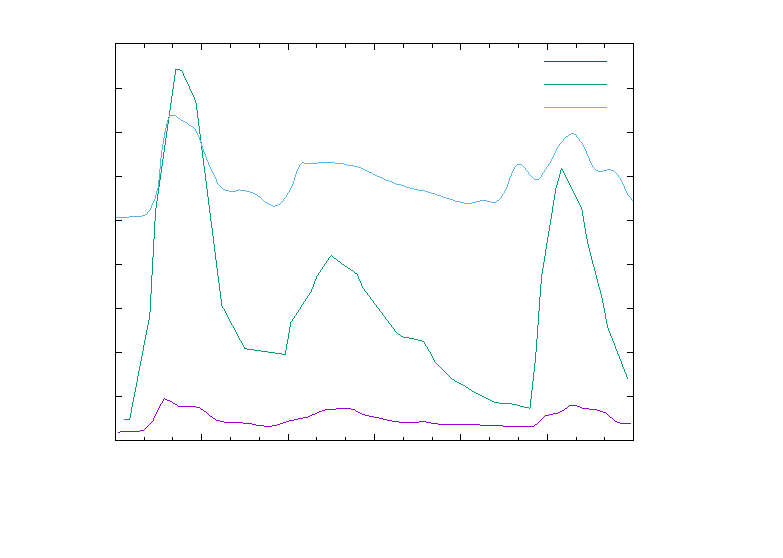
\includegraphics{../images/vw}}%
    \gplfronttext
  \end{picture}%
\endgroup

  \caption{Timeseries of the uncorrected \ch{NO2}, \ch{NO_x} and
    \ch{CO2} concentrations in the plume of a VW Pasat TDI.}
  \label{fig:vw-ts}
\end{figure}

%%% Local Variables:
%%% mode: latex
%%% TeX-master: "../Bachelor"
%%% End:

\cleardoubleoddstandardpage{}
\section{Conclusion and outlook}
\label{sec:conclusion}

This bachelor thesis was dedicated to further improve a \ch{NO} to
\ch{NO2} converter by testing \ch{NO_x} filtering capabilities of silica gel
behind the ozone generator. This was successfully proven. The
additional \ch{NO2} signal at the generator output could be removed
completely, while still achieving over \SI{200}{ppm} ozone
output. Moreover, the startup time seems manageable and lies in the
region of \SI{5}{\minute} after the start of the mercury lamp and the
pump of the ozone system. 

Furthermore, I could show that in a synthetic setting without \ch{NO2}
and precisely controlled \ch{NO} the measurement deviation from the
computed \ch{NO} concentrations lies in the per mille region. Hence,
there is a very high correlation between the measured and the computed
data. For measurements in ambient air it was necessary to research the
behavior of the system after turning the converter alternating.
Thereby drawbacks were investigated that \ch{NO} is still partly
converted to \ch{NO2} for \SI{2.5}{\minute} to \SI{3}{\minute} after
switching off the converter. This effect most likely arises from ozone
adsorption on the teflon walls which is only slowly removed after
turning off the converter. This has the effect that in a measurement
mode switching on and off the converter within approximately
\SI{1}{\minute} leads to an offset in the \ch{NO2} data.  The
adsorption effect is also supported by the measurement that the ozone
concentration seemed to indicate a proportionality to the reaction
tube length. If adsorption really is the reason, this would impact the
future design constraints of the converter. So far a standard
\SI{4}{\milli\meter} diameter teflon tube was used as reaction path,
which allowed for the necessary mixing of the gases and which could
easily be adapted to the necessary length of \SI{10}{\meter}. In order
to diminish the adsorption effects, the reaction path would have to be
shortened, while still keeping the dwell time constant. This could be
achieved by using a reaction tube with a larger diameter, as this
would reduce the surface area. However, a good mixing of the ozone
with the sample air still has to be guaranteed. Since the used pumps
only allow for laminar flows in the system, it might be the case that
the diameter becomes too large for an adequate mixing by diffusion. A
remedy could be the introduction of one or multiple jets behind the
ozone injection. This would allow for turbulences and improved mixing,
without unnessecarily increasing the teflon surface. Alternatively, a
shorter, thin mixing tube could be used, which then widens into a
reaction chamber. The adsorption research and possible alternative
designs of the reaction path are the natural next steps in the
development of the converter.

However, the adsorption effects have only to be taken into account, if
one wants to switch between \ch{NO_x} and \ch{NO2} measurements. If
one (or both) of the modes is (are) fixed, there are no discernible
adsorption effects. Since during vehicle measurements the actually
important quantity is the \ch{NO_x} concentration, the converter in
the current form is already ready for operation. Furthermore,
comparing the cavity data to the official data of the Heidelberg air
quality measurement station showed that using two measurement cells in
parallel avoids the difficulties introduced by the alternating
measurement mode.

The investigation of vehicel emissions showed that a true \ch{NO_x}
measurement instrument is necessary, as the average emission of
\ch{NO_x} per \ch{CO2} often lay a factor ten higher than the emission
of \ch{NO2} per \ch{CO2}. For a reliable conclusion of these emissions
a few more measurements are required. The peak \ch{NO_x} values
during the campaign lay in the region of \SI{4000}{ppb}, this is also
the region of the concentration of the injected ozone. Thus additional
measurements should be conducted to determine the \ch{NO} to \ch{NO2}
conversion ratio for these high concentrations. The effect of an
increased ozone flow should be studied, in order to see if it is a viable
solution for higher concentrations or if further oxidation processes
may arise.

All in all, in this thesis it was shown that indirect \ch{NO}
measurements are possible using this setup. For moderate
concentrations reliable \ch{NO_x} values can be achieved and with
slight adaptions even high ranging \ch{NO_x} values should be
determinable with a good accuracy. Thus in the near future the
converter should be ready for \ch{NO_x} vehicle measurements. There is
still some work to be done when one measurement cell should measure
\ch{NO2} and \ch{NO_x} alternatingly. In this case further studies
towards adsorption effects are necessary and the design of the
converter, especially the reaction volume, has to be reevaluated and
adapted. Still, this work succeeded in taking a next step towards a
robust implementation of this promising measurement technique.

%%% Local Variables:
%%% mode: latex
%%% TeX-master: "../Bachelor"
%%% End:

\cleardoubleoddstandardpage{}


\printbibliography[heading=bibintoc]

%%% Local Variables: 
%%% mode: latex
%%% TeX-master: "Bachelor"
%%% End: 



\cleardoubleoddstandardpage{}
\selectlanguage{german}
  
\subsubsection*{Erklärung}
\label{sub:Erklärung}

Ich versichere, dass ich diese Arbeit selbstständig verfasst und keine 
anderen als die angegebenen Quellen und Hilfsmittel verwendet habe.

\vspace{2\baselineskip}

Heidelberg, den 25.\ April 2016 \hspace{5em} \hrulefill

\selectlanguage{english}

%%% Local Variables: 
%%% mode: latex
%%% TeX-master: "../Bachelor"
%%% End: 


\end{document}

%%% Local Variables: 
%%% mode: latex
%%% TeX-master: t
%%% End: 
